\scsectionfamily{Часть 1 Стандарта OSTIS. Введение в интеллектуальные компьютерные системы нового поколения}
\label{part_intro}

\scsection[
\protect\scnidtf{Характеристики (параметры и способности) \textit{кибернетических систем}, определяющие их качество и, в частности, уровень их \textit{интеллекта}};
\protect\scnmonographychapter{Глава 1.1. Факторы, определяющие уровень интеллектуальности кибернетических систем. Этапы эволюции компьютерных систем в направлении повышения уровня их интеллектуальности}
]{Предметная область и онтология кибернетических систем}
\label{sd_sys_inform}
\begin{SCn}
	\scnsectionheader{Предметная область и онтология кибернетических систем}

	\begin{scnsubstruct}

		\scnheader{Предметная область кибернетических систем}
		\scniselement{предметная область}
		\begin{scnhaselementrolelist}{класс объектов исследования}
			\scnitem{кибернетическая система}
		\end{scnhaselementrolelist}

		\begin{scnhaselementrolelist}{класс объектов исследования}
			\scnitem{искусственная сущность}
			\scnitem{компьютерная система}
			\scnitem{простая кибернетическая система}
			\scnitem{индивидуальная кибернетическая система}
			\scnitem{кибернетическая система, встроенная в индивидуальную
				кибернетическую систему}
			\scnitem{многоагентная система}
			\scnitem{одноуровневая многоагентная система}
			\scnitem{коллектив индивидуальных кибернетических систем}
			\scnitem{иерархический коллектив индивидуальных кибернетических систем}
			\scnitem{информация, хранимая в памяти кибернетической системы}
			\scnitem{абстрактная память кибернетической системы}
			\scnitem{решатель задач кибернетической системы}
			\scnitem{действие кибернетической системы}
			\scnitem{задача}
			\scnitem{задача, решаемая кибернетической системой}
			\scnitem{навык}
			\scnitem{интерфейс кибернетической системы}
			\scnitem{физическая оболочка кибернетической системы}
			\scnitem{память кибернетической системы}
			\scnitem{процессор кибернетической системы}
			\scnitem{компьютер}
			\scnitem{качество кибернетической системы}
			\scnitem{гибридная кибернетическая система}
			\scnitem{приспособленность кибернетической системы к её
				совершенствованию}
			\scnitem{гибкость кибернетической системы}
			\scnitem{производительность кибернетической системы}
			\scnitem{надежность кибернетической системы}
			\scnitem{качество физической оболочки кибернетической системы}
			\scnitem{качество памяти кибернетической системы}
			\scnitem{интеллект}
			\scnitem{образованность кибернетической системы}
			\scnitem{интеллектуальная система}
			\scnitem{кибернетическая система, основанная на знаниях}
			\scnitem{кибернетическая система, управляемая знаниями}
			\scnitem{целенаправленная кибернетическая система}
			\scnitem{обучаемая кибернетическая система}
			\scnitem{социально ориентированная кибернетическая система}
			\scnitem{интеллектуальная компьютерная система}
			\scnitem{информация}
			\scnitem{сенсорная информация}
			\scnitem{качество решателя задач кибернетической системы}
			\scnitem{обучаемость кибернетической системы}
			\scnitem{стратифицированность кибернетической системы}
			\scnitem{рефлексивность кибернетической системы}
			\scnitem{синергетическая кибернетическая система}
			\scnitem{социализация кибернетической системы}
		\end{scnhaselementrolelist}

		\begin{scnhaselementrolelist}{исследуемое отношение}
			\scnitem{информация, хранимая в памяти кибернетической системы*}
			\scnitem{задача, решаемая кибернетической системой*}
			\scnitem{внешняя среда кибернетической системы*}
			\scnitem{среда кибернетической системы*}
			\scnitem{агент*}
		\end{scnhaselementrolelist}

		\scnidtf{Иерархическая система свойств (характеристик) кибернетических
			систем, определяющих общий (интегральный) уровень их качества}
		\scnidtf{Эволюционный подход к определению качества и, в частности,
			уровня интеллекта кибернетической системы}
		\scntext{аннотация}{Рассмотрена иерархическая система свойств (в т.ч.
			способностей) кибернетических систем, определяющих их качество и позволяющих
			сформулировать требования, которым должна удовлетворять высокоинтеллектуальная
			система (кибернетическая система с сильным интеллектом).Уровень качества
			кибернетических систем определяется достаточно большим набором свойств
			(параметров, характеристик) кибернетических систем, каждое из которых
			определяет уровень качества кибернетической системы в соответствующем аспекте
			(ракурсе), указывая (задавая) уровень развития конкретных  способностей и
			возможностей кибернетической системы. При этом важно подчеркнуть следующее:
			\begin{scnitemize}
				\item существенное значение имеет не столько сам набор свойств, а
				иерархия этих свойств, позволяющая уточнять (детализировать) направления
				проявления (реализации) каждого свойства
				\item существенное значение также имеет \uline{баланс} уровней развития
				различных свойств --- вклад разных свойств, обеспечивающих (определяющих)
				значение одного и того же свойства более высокого уровня иерархии, а значение
				этого свойства более высокого уровня может быть разным. Из этого следует, что
				не всегда следует акцентировать внимание на развитие некоторых свойств
				(характеристик). Нужен целостный, коллективный подход
				\item рассмотренная иерархия свойств кибернетических систем является
				общей как для естественных, так и для искусственных кибернетических систем
				\item приведенная иерархическая детализация свойств кибернетических
				систем (с помощью отношения \scnqqi{\textit{частное свойство*}} и отношения
				\textit{свойство-предпосылка*}), определяющих качество таких систем, (1) дает
				возможность четко определить направления совершенствования (развития)
				кибернетических систем и (2) дает ориентир (систему критериев) для обоснования
				конкретных предложений по совершенствованию компьютерных систем, а также для
				сравнения различных альтернативных предположений
				\item особое значение для развития кибернетических систем имеют такие
				их свойства, как стратифицированность, рефлексивность и социализация
				\item важное значение имеет не только совершенствование кибернетических
				систем в соответствии с иерархической системой их свойств, но и
				совершенствование (в том числе, детализация) самой этой иерархической системы
				свойств.
			\end{scnitemize}}

		\scntext{предисловие}{Свойства (способности), которым должны
			удовлетворять \textit{интеллектуальные системы}, рассматриваются в целом ряде
			публикаций. Тем не менее, для \uline{практической} реализации
			\textit{компьютерных систем}, обладающих указанными свойствами (способностями),
			т.е. \textit{интеллектуальных компьютерных систем}, необходимо детализировать
			(уточнить) эти \textit{свойства}, пытаясь свести их к более конструктивным,
			прозрачным и понятным для реализации свойствам.}

		\begin{scnrelfromset}{рассматриваемые вопросы}
			\scnfileitem{По каким свойствам (параметрам, характеристикам,
					способностям) кибернетических систем можно оценивать уровень их качества.}
			\scnfileitem{Можно ли считать уровень развития какого-либо
					свойства (способности) кибернетической системы, т.е. значение какого-либо ее
					параметра (характеристики) оценкой уровня качества кибернетической системы по
					соответствующему аспекту.}
			\scnfileitem{Может ли какое-либо свойство кибернетических
					систем определять (влиять на) значение сразу нескольких свойств более высокого
					уровня иерархии.}
			\scnfileitem{Какими отношениями свойства кибернетических
					систем связаны со свойствами более низкого и, соответственно, более высокого
					уровня иерархии.}
			\scnfileitem{Зачем нужна такая иерархия свойств, определяющих
					качество кибернетических систем и позволяющих детализировать (уточнять) то,
					какими свойствами определяется уровень (степень) развития каждого свойства
					(значение каждого свойства) за исключением свойств, которые условно можно
					считать элементарными, не требующими детализации (по крайнем мере, пока).}
			\scnfileitem{Может ли иерархия свойств, определяющих качество
					кибернетических систем, быть критерием оценки и выбора того или иного подхода к
					построению интеллектуальных компьютерным систем.}
			\scnfileitem{Какими свойствами (способностями) должна обладать
					кибернетическая система, имеющая высокий уровень интеллекта.}
			\scnfileitem{Какими свойствами определяется уровень интеллекта
					многоагентной кибернетической системы.}
			\scnfileitem{Как связан уровень интеллекта многоагентной
					системы с уровнем интеллекта агентов, входящих в ее состав.}
			\scnfileitem{Почему, например, не каждый коллектив
					высокоинтеллектуальных людей демонстрирует высокий уровень интеллекта самого
					коллектива.}
			\scnfileitem{Какими дополнительными свойствами кроме
					достаточно высокого уровня интеллекта должны обладать агенты многоагентных
					систем для обеспечения высокого уровня интеллекта самой многоагентной системы
					как самостоятельной целостной кибернетической системы.}
			\scnfileitem{Как зависит уровень интеллекта многоагентной
					системы от организации взаимодействия между агентами, например, от
					использования централизованного или децентрализованного управления.}
		\end{scnrelfromset}

		\begin{scnrelfromvector}{ключевые знаки}
			\scnitem{кибернетическая система}
			\begin{scnindent}
				\begin{scnsubdividing}
					\scnitem{естественная кибернетическая система}
					\scnitem{компьютерная система}
                    \begin{scnindent}
                        \scnidtf{искусственная кибернетическая система}
                    \end{scnindent}
					\scnitem{естественно-искусственная кибернетическая система}
                    \begin{scnindent}
                        \scnidtf{кибернетическая система, являющаяся симбиозом компонентов как
                            естественного, так и искусственного происхождения}
                    \end{scnindent}
				\end{scnsubdividing}
            \end{scnindent}
			\scnitem{качество кибернетической системы}
			\scnitem{физическая оболочка кибернетической системы}
			\scnitem{качество физической оболочки кибернетической системы}
			\scnitem{интеллект}
				\begin{scnindent}
					\scnidtf{уровень интеллекта кибернетическойсистемы}
					\scnidtf{интеллектуальность}
				\end{scnindent}
			\scnitem{интеллектуальная система}
				\begin{scnindent}
					\scnidtf{интеллектуальная кибернетическая система}
					\scnsuperset{интеллектуальная компьютерная система}
				\end{scnindent}
			\scnitem{информация, хранимая в памяти кибернетической системы}
			\scnitem{качество информации, хранимой в памяти кибернетической
				системы}
			\scnitem{база знаний}
			\scnitem{смысловое представление информации в памяти кибернетической
				системы}
			\scnitem{решатель задач кибернетической системы}
			\scnitem{качество решателя задач кибернетической системы}
			\scnitem{память кибернетической системы}
			\scnitem{качество памяти кибернетической системы}
			\scnitem{обучаемость кибернетической системы}
			\scnitem{гибкость кибернетической системы}
			\scnitem{стратифицированность кибернетической системы}
			\scnitem{рефлексивность кибернетической системы}
				\begin{scnindent}
					\scnidtf{уровень рефлексии кибернетической системы}
				\end{scnindent}
			\scnitem{многоагентная система}
			\scnitem{качество многоагентной системы}
			\scnitem{унифицированность агентов многоагентной системы}
			\scnitem{семантическая совместимость агентов многоагентной системы}
			\scnitem{социализация кибернетической системы}
				\begin{scnindent}
					\scnidtf{способность кибернетической системы своей внутренней и внешней деятельностью обеспечивать
						высокий уровень интеллекта тех многоагентных систем, членом (агентом) которых
						она является}
				\end{scnindent}
		\end{scnrelfromvector}

		\begin{scnrelfromvector}{библиография}
			\scnitem{\cite{Viner1952}}
			\scnitem{\cite{Pospelov1989}}
			\scnitem{\cite{Finn2008}}
			\scnitem{\cite{YarushinaHS}}
			\scnitem{\cite{RedkoV2019}}
		\end{scnrelfromvector}

		\begin{scnreltovector}{конкатенация сегментов}
			\scnitem{Уточнение понятия кибернетической системы}
			\scnitem{Комплекс свойств, определяющий общий уровень качества
				кибернетической системы}
			\scnitem{Комплекс свойств, определяющих качество физической оболочки
				кибернетической системы}
			\scnitem{Комплекс свойств, определяющих уровень интеллекта
				кибернетической системы}
			\scnitem{Комплекс свойств, определяющий качество информации, хранимой в
				памяти кибернетической системы}
			\scnitem{Комплекс свойств, определяющих качество решателя задач
				кибернетической системы}
			\scnitem{Комплекс свойств, определяющих уровень обучаемости
				кибернетической системы}
			\scnitem{Комплекс свойств, определяющих качество многоагентной системы}
			\scnitem{Комплекс свойств, определяющих уровень социализации
				кибернетической системы как фактора существенного повышения уровня ее
				обучаемости, а также фактора существенного повышения качества всех тех
				многоагентных систем, в состав которых входит данная кибернетическая система}
		\end{scnreltovector}

		\newpage
		
		\scnsegmentheader{Уточнение понятия кибернетической системы}
\begin{scnsubstruct}
    \scnheader{кибернетическая система}
    \scnidtf{cистема, которая способна \uline{управлять} своими \uline{действиями},
        адаптируясь к изменениям состояния внешней среды (среды своего обитания) в
        целях самосохранения (сохранения своей целостности и комфортности
        существования путем удержания своих жизненно  важных параметров в определенных
        рамках комфортности) и/или в целях формирования определенных реакций
        (воздействий на внешнюю среду) в ответ на определенные стимулы (на определенные
        ситуации или события во внешней среде), а также которая способна (при
        соответствующем уровне развития) эволюционировать в направлении:
        \begin{scnitemize}
            \item изучения своей внешней среды как минимум для предсказания последствий
            своих воздействий на внешнюю среду, а также для предсказания изменений внешней
            среды, которые не зависят от собственных воздействий;
            \item изучения самой себя и, в частности, своего взаимодействия с внешней
            средой;
            \item создания технологий (методов и средств), обеспечивающих изменение своей
            внешней среды (условий своего существования) в собственных интересах.
        \end{scnitemize}
    }
    \scnidtf{адаптивная система}
    \scnidtf{целенаправленная (целеустремленная) система}
    \scnidtf{активный субъект самостоятельной деятельности}
    \scnidtf{материальная сущность, способная целенаправленно (в своих интересах)
        воздействовать	на среду своего обитания  как минимум для сохранения своей
        целостности, жизнеспособности, безопасности}
    \scntext{примечание}{Уровень (степень) адаптивности, целенаправленности, активности у
        систем, основанных на обработке информации может быть самым
        различным.}\scnidtf{система, организация функционирования которой основано на
        обработке информации о той среде, в которой существует эта система}
    \scnidtf{материальная сущность, способная к активной  целенаправленной
        деятельности, которая  на определенном уровне развития указанной сущности
        становится осмысленной, планируемой, преднамеренной деятельностью}
    \scnidtf{субъект, способный на самостоятельное выполнение некоторых внутренних
        и внешних  действий либо порученных извне, либо инициированных самим субъектом}
    \scnidtf{сущность, способная выполнять роль субъекта деятельности}
    \scnidtf{естественная или искусственно созданная система, способная мониторить
        и анализировать свое состояние и состояние окружающей среды, а также способная
        достаточно активно воздействовать на собственное на собственное состояние и на
        состояние окружающей среды}
    \scnidtf{система, способная в достаточной степени самостоятельно
        взаимодействовать со своей средой , решая различные задачи}
    \scnidtf{система, основанная на обработке информации}
    \newpage\scnrelto{ключевой знак}{\cite{Glushkov1979}}
    \scniselement{статья}
    \bigskip

    \scnsegmentheader{Типология кибернетических систем}
    \begin{scnsubstruct}
        \scnheader{кибернетическая система}
        \scnrelfrom{разбиение}{Признак естественности или искусственности
            кибернетических систем}
        \begin{scneqtoset}

            \scnitem{естественная кибернетическая система \\\scnidtf{кибернетическая
                    система естественного происхождения}
                \scnsuperset{человек}
            }
            \scnitem{компьютерная система \\\scnidtf{искусственная кибернетическая система}
                \scnidtf{кибернетическая система искусственного происхождения}
                \scnidtf{технически реализованная кибернетическая система}
            }
            \scnitem{симбиоз естественных и искусственных кибернетических
                систем
                \\\scnidtf{кибернетическая система, в состав которой входят компоненты
                    как естественного, так и искусственного происхождения}
                \scnsuperset{сообщество компьютерных систем и людей}
            }

        \end{scneqtoset}
        \scnheader{искусственная сущность}
        \scnidtf{артефакт}
        \scnidtf{сущность, являющаяся либо результатом человеческой деятельности, либо
            частью самой этой деятельности}
        \scnidtf{сущность искусственного происхождения}
        \scnidtf{антропогенная сущность}
        \scnsuperset{научно-техническое знание}
        \scnidtf{знание, приобретенное в результате научно-технической деятельности
            человеческого общества}
        \scnsuperset{материальная искусственная сущность}
        \scnsuperset{компьютерная система}
        \scnheader{компьютерная система}
        \scnidtf{искусственная кибернетическая система}
        \scntext{примечание}{Особенностью компьютерных систем является то, что они могут
            выполнять роль	не только продуктов соответствующих действий по реализации этих
            систем, но и сами являются \textit{субъектами*}, способными выполнять
            (автоматизировать) широкий спектр действий. При этом интеллектуализация этих
            систем существенно расширяет этот спектр. \textit{См. интеллектуальная
                компьютерная система}.}\scnidtf{технически реализованная кибернетическая
            система}
        \scnidtf{искусственная кибернетическая система}
        \scnsubset{кибернетическая система}
        \scnsuperset{современная компьютерная система традиционного вида}
        \scnsuperset{современная интеллектуальная компьютерная система}
        \scnsuperset{интеллектуальная компьютерная система следующего поколения}
        \scnsuperset{ostis-система}
        \scntext{примечание}{Основной тенденцией эволюции компьютерных систем является
            повышение уровня их интеллектуальности.}\begin{scnrelfromset}{особенность}

            \scnfileitem{Ориентация на принципиально новые компьютеры}
            \scnfileitem{Cущественное повышение уровня интеллекта}

        \end{scnrelfromset}
        \newpage\scnrelfrom{разбиение}{Структурная классификация кибернетических
            систем}
        \begin{scneqtoset}
            \scnitem{простая кибернетическая система}
            \scnitem{индивидуальная кибернетическая система}
            \scnitem{многоагентая система
                \begin{scnsubdividing}
                    \scnitem{одноуровневый коллектив кибернетических систем}
                        \begin{scnindent}
                            \scnidtf{многоагентная система, агентами которой не могут быть многоагентные системы}
                        \end{scnindent}
                    \scnitem{иерархический коллектив кибернетических систем}
                        \begin{scnindent}
                            \scnidtf{многоагентная система, по крайней мере одним	агентом которой является многоагентная система}
                        \end{scnindent}
                \end{scnsubdividing}
                \begin{scnsubdividing}
                    \scnitem{коллектив из простых кибернетических систем}
                        \begin{scnindent}
                            \scntext{примечание}{Такой коллектив может быть либо одноуровневым, либо иерархическим коллективом}
                        \end{scnindent}
                    \scnitem{коллектив из индивидуальных кибернетических систем}
                    \scnitem{коллектив из индивидуальных и простых кибернетических систем}
                \end{scnsubdividing}
            }
        \end{scneqtoset}
        \scnheader{кибернетическая система}
        \scnrelfrom{разбиение}{Классификация кибернетических систем по признаку наличия
            надсистемы и роли в рамках этой надсистемы}
        \begin{scneqtoset}
            \scnitem{кибернетическая система, не являющаяся частью никакой другой
                кибернетической системы}
                \begin{scnindent}
                    \scnidtf{кибернетическая система, не имеющая надсистем}
                \end{scnindent}
            \scnitem{кибернетическая система, встроенная в индивидуальную кибернетическую
                систему}
            \scnitem{агент многоагентной системы}
                \begin{scnindent}
                    \scnidtf{кибернетическая система, являющаяся агентом одной или нескольких многоагентных систем}
                \end{scnindent}
        \end{scneqtoset}

        \scnheader{простая кибернетическая система}
        \scnidtf{\textit{кибернетическая система}, уровень развития которой находится
            ниже уровня \textit{индивидуальных кибернетических систем} и которая является
            специализированным средством обработки информации специализированным решателем
            задач, реализующим (интерпретирующим) чаще всего один \textit{метод} решения
            задач и, соответственно, решающим только \textit{задачи} заданного
            \textit{класса задач}}
        \scnidtf{специализированный \textit{решатель задач}}
        \scntext{примечание}{\textit{простая кибернетическая система} может быть
            \textit{компонентом*}, встроенным в \textit{индивидуальную кибернетическую
            систему}, а также может быть \textit{агентом*} \textit{многоагентной системы}, являющейся коллективом из простых
            кибернетических систем}
            
        \scnheader{индивидуальная кибернетическая система}
        \scnidtf{условно выделенный уровень развития \textit{кибернетических систем}, в
            основе которого лежит переход от \textit{специализированного решателя задач к
            индивидуальному решателю}, обеспечивающему интерпретацию произвольного
            (нефиксированного) набора \textit{методов} (программ) решения задач при
            условии, если эти \textit{методы} введены (загружены, записаны) в
            \textit{память} \textit{кибернетической системы}}
        \scnidtf{кибернетическая система, способная быть самостоятельной}
        \scntext{пояснение}{Признаками индивидуальных кибернетических систем
            являются:
            \begin{scnitemize}
                \item наличие \textit{памяти}, предназначенной для хранения как минимум
                интерпретируемых \textit{методов} (программ)  и обеспечивающей корректировку
                (редактирование) хранимых \textit{методов}, а также их удаление  из
                \textit{памяти} и ввод (запись) в \textit{память} новых \textit{методов};
                \item легкая возможность перепрограммировать  \textit{кибернетическую систему}
                на решение других задач, что обеспечивается наличием \textit{универсальной
                    модели решения задач} и, соответственно, \textit{универсальным интерпретатором
                    \uline{любых} моделей}, представленных (записанных) на соответствующем
                \textit{языке};
                \item наличие пусть даже простых средств коммуникации (обмена информацией) с
                другими \textit{кибернетическими системами} (например, с людьми);
                \item способность входить в различные \textit{коллективы кибернетических
                    систем}.
            \end{scnitemize}
        }\scntext{примечание}{класс \textit{индивидуальных кибернетических систем}  это
            определенный этап эволюции кибернетических систем, означающий переход к
            кибернетическим системам, которые способны самостоятельно
            выживать}\scnidtf{самостоятельная автономная, целостная кибернетическая
            системам}
        \scnidtf{субъект деятельности}
        \scntext{примечание}{\textit{индивидуальная кибернетическая система} может быть
            агентом (членом) многоагентной системы (членом коллектива индивидуальных
            кибернетических систем), но некоторые многоагентные системы могут состоять из
            агентов , не являющихся  \textit{индивидуальными кибернетическими системами},
            представляющих собой простые специализированные кибернетические системы,
            выполняющие достаточно простые действия (\cite{Stefanuk},
            %\bigspace
            \cite{fonNeuman})}\scnidtf{кибернетическая система, которая обладает
            достаточной самостоятельностью (целостностью), но не является коллективом таких
            самостоятельных  кибернетических систем}
        \scnidtf{минимальная самостоятельная (самодостаточная, в известной степени
            автономная) кибернетическая система}
        \scnidtf{индивидуальный субъект}
        \scnheader{кибернетическая система, встроенная в индивидуальную кибернетическую
            систему}
        \scnrelsuperset{пример}{sc-агент ostis-системы}
        \scnrelsuperset{пример}{решатель задач ostis-системы}
        \scnheader{многоагентная система}
        \scnidtf{коллектив взаимодействующих автономных кибернетических систем, имеющих
            общую среду обитания (жизнедеятельности)}
        \begin{scnsubdividing}

            \scnitem{одноуровневая многоагентная система}
            \scnitem{иерархическая многоагентная система}

        \end{scnsubdividing}
        \scnheader{одноуровневая многоагентная система}
        \scnidtf{специализированное средство решения задач, реализующее либо
            \uline{одну} модель параллельного (распределенного) решения задач
            соответствующего класса, либо комбинацию \uline{фиксированного числа} разных и
            параллельно реализованных моделей решения задач}
        \begin{scnsubdividing}

            \scnitem{одноуровневая однородная многоагентная система}
            \scnitem{одноуровневая неоднородная многоагентная система}

        \end{scnsubdividing}
        \scnheader{коллектив индивидуальных кибернетических систем}
        \scnsubset{многоагентная система}
        \scnidtf{многоагентная система, агентами (членами) которой являются
            \uline{индивидуальные}(!) кибернетические системы}
        \begin{scnsubdividing}

            \scnitem{коллектив людей}
                \begin{scnindent}
                    \scnidtf{человеческое сообщество}
                \end{scnindent}
            \scnitem{сообщество компьютерных систем и людей}

        \end{scnsubdividing}
        \scnheader{иерархический коллектив индивидуальных кибернетических систем}
        \scnidtf{многоагентная система, агентами (членами) которой могут быть:
            \begin{scnitemize}

                \item индивидуальные кибернетические системы;
                \item коллективы индивидуальных кибернетических систем;
                \item коллективы, состоящие из индивидуальных кибернетических систем и
                коллективов индивидуальных кибернетических систем и т.д.
            \end{scnitemize}
        }
        \bigskip
    \end{scnsubstruct}
    \scnsegmentheader{Структура кибернетической системы}
    \begin{scnsubstruct}
        \scnheader{кибернетическая система}
        \begin{scnrelfromset}{обобщенная декомпозиция}

            \scnitem{информация, хранимая в памяти кибернетической системы}
            \scnitem{абстрактная память кибернетической системы}
            \scnitem{решатель задач кибернетической системы}
            \scnitem{физическая оболочка кибернетической системы}

        \end{scnrelfromset}
        \scnheader{информация, хранимая в памяти кибернетической системы}
        \scnidtf{информация, хранимая в памяти \textit{кибернетической системы} и
            представляющая собой информационную модель среды, в которой действует
            (существует, функционирует) эта \textit{кибернетическая система}}
        \scnidtf{текущее состояние памяти кибернетической системы}
        \scnidtf{текущее состояние внутренней (информационной) среды кибернетической
            системы}
        \scnrelto{второй домен}{информация, хранимая в памяти кибернетической системы*}
        \begin{scnindent}
            \scniselement{бинарное отношение}
            \scniselement{ориентированное отношение}
        \end{scnindent}
        \scnheader{абстрактная память кибернетической системы}
        \scnidtf{внутренняя абстрактная информационная среда кибернетической системы,
            представляющая собой динамическую информационную  конструкцию, каждое состояние
            которой есть не что иное, как информация , хранимая в памяти кибернетической
            системы в соответствующий момент времени}
        \scnidtf{абстрактная динамическая модель памяти кибернетической системы}
        \scnsubset{динамическая информационная конструкция}
        \begin{scnindent}
            \scnidtf{процесс преобразования информационной конструкции}
        \end{scnindent}
        \scnheader{решатель задач кибернетической системы}
        \scnidtf{совокупность всех навыков (умений), приобретенных кибернетической
            системой к рассматриваемому моменту}
        \scnidtf{встроенный в кибернетическую систему субъект, способный выполнять
            целенаправленные (осознанные) действия во внешней среде этой кибернетической
            системы, а также в её внутренней среде (в абстрактной памяти)}
        \scnheader{действие кибернетической системы}
        \scnsubset{действие}
        \scnidtf{целенаправленное (осознанное) действие, выполняемое кибернетической
            системой, а точнее, её решателем задач}
        \begin{scnsubdividing}

            \scnitem{внешнее действие кибернетической системы}
            \begin{scnindent}
                \scnidtf{действие, выполняемое кибернетической системой в её внешней среде}
                \scnidtf{поведенческое действие}
            \end{scnindent}
            \scnitem{действие кибернетической системы, выполняемое в собственной физической
                оболочке}
            \scnitem{действие кибернетической системы, выполняемое в собственной
                абстрактной памяти}
            \begin{scnindent}
                \scnidtf{речь идёт о действиях, направленных на
                    преобразование информации, хранимой в памяти, но никак не на преобразование
                    физической памяти (физической оболочки абстрактной памяти)}
            \end{scnindent}
        \end{scnsubdividing}
        \newpage\scntext{примечание}{Каждое \uline{сложное} действие,выполняемое
            кибернетической системой вне собственный абстрактной памяти, включает в себя
            поддействия, выполняемые в указанной абстрактной памяти. Это означает, что все
            внешние действия кибернетической системы \uline{управляются} внутренними её
            действиями (действиями в абстрактной памяти).}\scnheader{задача}
        \scnidtf{спецификация действия}
        \scnidtf{формулировка задачи с различной степенью детализации (уточнения)
            специфицируемого (описываемого) действия, в состав которой может входить:
            \begin{scnitemize}

                \item описание цели (целевой ситуации);
                \item указание объектов (аргументов) действия;
                \item указание типа действия (класса действий, которому принадлежит данное
                действие);
                \item указание субъекта действия;
                \item указание инструмента (средств) выполненного действия;
                \item и др.
            \end{scnitemize}
        }
        \scntext{примечание}{Процесс решения задачи и действие, специфицируемое этой задачей
            (точнее, процесс выполнения этого действия) суть одно и то
            же.}
        \scnheader{задача, решаемая кибернетической системой}
        \scnidtf{задача, решаемая соответствующей кибернетической системой}
        \scnidtf{Второй домен отношения быть задачей, решаемой заданной кибернетической
            системой*}
        \scnrelboth{следует отличать}{задача, решаемая кибернетической системой*}
        \begin{scnindent}
            \scnidtf{быть задачей, решаемой заданной кибернетической системой*}
        \end{scnindent}
        \begin{scnsubdividing}

            \scnitem{задача, решаемая кибернетической системой во внешней среде}
                \begin{scnindent}
                    \scnidtf{внешняя задача кибернетической системы}
                    \scnidtf{задача, направленная на изменение состояния внешней среды
                        соответствующей кибернетической системы, но включающая в себя (в качестве
                        подзадач) задачи, решаемые в памяти кибернетической системы, например:
                        \begin{scnitemize}

                            \item интерфейсные задачи (анализ первичный информации о текущем состоянии
                            внешней среды),
                            \item cенсо-моторную координацию выполнения сложных действий во внешней среде,
                            состоящих из большого количества частных (более простых) действий, находящихся
                            на разных уровнях иерархии,
                            \item задачи планирования целенаправленного поведения во внешней среде,
                            \item задачи принятия решений.
                        \end{scnitemize}
                    }
                \end{scnindent}
            \scnitem{задача, решаемая кибернетической системой в собственной физической
                оболочке}
            \scnitem{задача решаемая кибернетической системой в абстрактной
                памяти}
                \begin{scnindent}
                    \scnidtf{задача, полностью решаемая в памяти кибернетической системы и
                        направленная на изменение состояния информации, хранимой в памяти
                        кибернетической системы}
                    \scnidtf{внутренняя задача кибернетической системы}
                \end{scnindent}

        \end{scnsubdividing}
        \scnheader{навык}
        \scnsubset{знание}
        \scntext{пояснение}{знание частного вида, содержащее (1) некоторый метод --
            знание о том, как можно решать задачи, принадлежащие соответствующему множеству
            задач, (2) полное знание о том, как указанный метод следует интерпретировать
            (реализовывать), декомпозируя исходные задачи на подзадачи и, в конечном счёте
            на элементарные действия, выполняемые \textit{процессором кибернетической
                системы}}\scnidtf{умение}
        \scnidtf{методы и средства, обеспечивающие способность \textit{кибернетической
                системы} решать некоторое множество задач (выполнять некоторое множество
            действий)}
        \scnheader{интерфейс кибернетической системы}
        \scnidtf{условно выделяемый компонент \textit{решателя задач кибернетической
                системы}, обеспечивающий решение \textit{интерфейсных задач}, направленных на
            \uline{непосредственную} реализацию взаимодействия \textit{кибернетической
                системы} с её \textit{внешней средой}}
        \scnidtf{решатель интерфейсных задач кибернетической системы}
        \scnrelto{обобщенная часть}{решатель задач кибернетической системы}
        \scnrelboth{следует отличать}{физическое обеспечение интерфейса кибернетической
            системы}
            \begin{scnindent}
                \scnrelto{обобщенная часть}{физическая оболочка кибернетической системы}
            \end{scnindent}
        \scnheader{физическая оболочка кибернетической системы}
        \begin{scnrelfromset}{обобщенная декомпозиция}

            \scnitem{память кибернетической системы}
            \scnitem{процессор кибернетической системы}
            \scnitem{физическое обеспечение интерфейса кибернетической системы}
            \begin{scnindent}   
                \scnidtf{аппаратное обеспечение интерфейса кибернетической системы с её
                    внешней средой}
                \begin{scnrelfromset}{обобщенная декомпозиция}

                    \scnitem{сенсорная подсистема физической оболочки кибернетической системы}
                    \scnitem{эффекторная подсистема физической оболочки кибернетической системы}

                \end{scnrelfromset}
            \end{scnindent}
            \scnitem{корпус кибернетической системы}
        \end{scnrelfromset}

        \scnheader{физическая оболочка кибернетической системы}
        \scnidtf{часть кибернетической системы, являющаяся посредником	между её
            внутренней средой (памятью, в которой хранится и обрабатывается информация
            кибернетической системы) и её внешней средой}
        \scnrelto{второй домен}{физическая оболочка кибернетической системы*}
        \begin{scnindent}
            \scniselement{бинарное отношение}
            \scniselement{ориентированное отношение}
        \end{scnindent}
        
        \scnheader{память кибернетической системы}
        \scnidtf{физическая оболочка (реализация) абстрактной \textit{памяти
                кибернетической системы} -- внутренней среды \textit{кибернетической системы},
            в рамках которой \textit{кибернетическая система} формирует и использует
            (обрабатывает) информационную модель своей внешней среды}
        \scntext{примечание}{Не каждая \textit{кибернетическая система} имеет
            \textit{память}. В \textit{кибернетических системах}, которые не имеют
            \textit{памяти}, обработка информации сводится к обмену сигналами между
            компонентами этих систем. Появление в \textit{кибернетических системах} памяти
            как среды для централизованного  хранения и обработки \textit{информации}
            является важнейшим этапом их эволюции. Дальнейшая эволюция
            \textit{кибернетических систем} во многом определяется:
            \begin{scnitemize}

                \item \textit{качеством памяти} как среды для хранения и обработки информации;
                \item качеством информации (информационной модели), хранимой в памяти
                кибернетической системы;
            \end{scnitemize}
        }\scnidtf{компонент кибернетической системы, в рамках которого
            \textit{кибернетическая система} осуществляет отображение (формирование
            информационной модели) среды своего существования, а также использование этой
            информационной модели для управления собственным поведением в указанной среде}
        \scnidtf{физическая оболочка для хранения информации, которую кибернетическая
            система приобретает и обрабатывает (т.е. меняет состояния этой информации)}
        \scnidtf{физическая (аппаратная) реализация \uline{внутренней} среды
            кибернетической системы, каковой является среда существования  информации,
            накапливаемой и непосредственно используемой решателем задач этой
            кибернетической системы}
        \newpage\scntext{примечание}{Сам факт появления в кибернетической системе памяти,
            которая (1) обеспечивает представление различного виды информации о среде, в
            рамках которой кибернетическая система решает различные задачи (выполняет
            различные действия), (2) обеспечивает хранение достаточно полной информационной
            модели указанной среды (достаточно полной для реализации своей деятельности),
            (3) обеспечивает высокую степень гибкости указанной хранимой в памяти
            информационной модели среды жизнедеятельности (т.е. лёгкость внесения изменений
            в эту информационную модель), существенно повышает уровень адаптивности
            кибернетической системы к различным изменениям своей
            среды.}\scntext{примечание}{появление  \uline{\textit{памяти}} в кибернетических
            системах является основным признаком перехода от простых  автоматов к
            компьютерным системам, от роботов 1-го поколения к роботам следующих
            поколений}\scnidtf{физическая реализация хранилища информации, которую
            приобрела (накопила) к текущему моменту соответствующая кибернетическая
            система}
        \scnidtf{физическая оболочка внутренней абстрактной информационной среды
            кибернетической системы}
        \scnidtf{среда хранения и обработки информации}
        \scnidtf{запоминающая среда}
        \scnidtf{среда хранения и обработки информационных конструкций}
        \scntext{примечание}{Принципы организации памяти кибернетической системы могут быть
            разными (ассоциативная, адресная, структурно фиксированная/структурно
            перестраиваемая, нелинейная/линейная). От организации памяти во многом зависит
            её качество.}
        \scnheader{кибернетическая система}
        \scnrelfrom{уровни эволюции}{Уровни структурной эволюции кибернетических систем}
        \begin{scnindent}
            \begin{scneqtovector}

                \scnitem{простая кибернетическая система, не имеющая памяти}
                \scnitem{простая кибернетическая система, имеющая память}
                \scnitem{одноуровневый коллектив, не имеющий общей памяти и состоящий из
                    простых кибернетических систем, не имеющих памяти}
                \scnitem{одноуровневый коллектив, не имеющий общей памяти и состоящий из
                    простых кибернетических систем, имеющих память}
                \scnitem{иерархический коллектив,  имеющий общую память и состоящий из простых
                    кибернетических систем}
                \scnitem{индивидуальная кибернетическая система}
                    \begin{scnindent}
                        \scntext{примечание}{Каждая \textit{индивидуальная кибернетическая система} содержит \textit{память},
                                имеющую достаточно высокий уровень качества}
                    \end{scnindent}
                \scnitem{одноуровневый коллектив индивидуальных кибернетических систем, не
                    имеющий общей памяти}
                \scnitem{одноуровневый коллектив индивидуальных кибернетическая систем, имеющий
                    общую память }
                \scnitem{иерархический коллектив из индивидуальных кибернетических систем, не
                    имеющий общей памяти}
                \scnitem{иерархический коллектив из индивидуальных кибернетических систем,
                    имеющий общую память}
            \end{scneqtovector}
        \end{scnindent}

        \scnheader{процессор кибернетической системы}
        \scnidtf{физически (аппаратно реализованный) интерпретатор хранимых в памяти
            кибернетической системы методов (программ), соответствующих базовой (для данной
            кибернетической системы) модели решения задач, т.е. такой модели решения задач,
            которая для данной кибернетической системы является моделью решения задач
            самого нижнего уровня и, следовательно, не может быть интерпретирована с
            помощью другой модели решения задач, используемой этой же кибернетической
            системой, а может быть проинтерпретирована либо путем аппаратной реализации
            такого интерпретатора, либо путём его программной реализации, например, на
            современных компьютерах, но в последнем случае, кроме собственного
            интерпретатора, необходимо также построить модель памяти реализуемой
            кибернетической системы}
        \scnidtf{физически  реализованные средства, обеспечивающие выполнение
            элементарных  действий, направленных на изменение состояния памяти
            кибернетической системы (на изменение информации, хранимой в этой памяти)}
        \scnidtf{движок(мотор) кибернетической системы}
        \scnrelto{второй домен}{процессор кибернетической системы*}
        \begin{scnindent}
            \scnidtftext{пояснение}{бинарное ориентированное отношения, каждая пара
                которого связывает знак кибернетической системы со знаком её процессора}
            \scniselement{бинарное отношение}
            \scniselement{ориентированное отношение}
        \end{scnindent}

        \scnheader{компьютер}
        \scnsubset{физическая оболочка кибернетической системы}
        \scnidtf{физическая оболочка искусственной кибернетической системы}
        \scnidtf{аппаратное обеспечение компьютерной системы}
        \scnidtf{hardware of computer system}
        \scnsuperset{компьютер для интеллектуальных систем}
        \begin{scnindent}
            \scnidtf{компьютер, ориентированный на реализацию интеллектуальных компьютерных
                систем}
            \scntext{примечание}{Развитие рынка интеллектуальных компьютерных систем существенно
                сдерживается неприспособленностью современного поколения компьютеров к
                реализации на их основе интеллектуальных компьютерных систем. Попытки создания
                компьютеров, приспособленных к реализации интеллектуальных компьютерных систем,
                не привели к успеху, т.к. эти проекты были направлены на выполнение отдельных
                (частных) требований, предъявляемых к физическому (аппаратному) уровню
                интеллектуальных систем, что неминуемо приводило к приспособленности
                создаваемых компьютеров к реализации не всего многообразия интеллектуальных
                компьютерных систем, а только некоторых подмножеств таких систем. Указанные
                подмножества интеллектуальных компьютерных систем в основном определялись
                ориентацией на конкретные используемые модели решения интеллектуальных задач,
                тогда, как важнейшим фактором, определяющим уровень интеллекта кибернетических
                систем (в том числе, и компьютерных систем), является их универсальность в
                плане многообразия используемых моделей решения задач. Следовательно, компьютер
                для интеллектуальных компьютерных систем должен быть эффективным аппаратным
                интерпретатором любых моделей решения задач (как интеллектуальных задач, так и
                достаточно простых задач, т.к. интеллектуальная система должна уметь решать
                любые задачи).}\scnidtf{компьютер, приспособленный к реализации
                интеллектуальных компьютерных систем}
            \scnidtf{универсальный компьютер для интеллектуальных систем}
            \scnidtf{компьютер, обеспечивающий интерпретацию любых моделей решения задач}
        \end{scnindent}
        \bigskip
    \end{scnsubstruct}
    \scnsegmentheader{Семейство отношений, заданных на множестве кибернетических
        систем}
    \begin{scnsubstruct}
        \scnheader{отношение, заданное на множестве кибернетических систем}
        \scnhaselement{память кибернетической системы*}
        \scnhaselement{процессор кибернетической системы*}
        \scnhaselement{член коллектива*}
        \scnhaselement{внешняя среда кибернетической системы*}
        \scnhaselement{сенсор кибернетической системы*}
        \scnhaselement{эффектор кибернетической системы*}
        \scnhaselement{физическая оболочка кибернетической системы*}
        \scnhaselement{информация, хранимая в памяти кибернетической системы*}
        \scnhaselement{абстрактная память кибернетической системы*}
        \scnhaselement{часть*}
        \begin{scnindent}
            \scnsuperset{встроенная кибернетическая система*}
        \end{scnindent}

        \scnheader{информация, хранимая в памяти кибернетической системы*}
        \scnidtf{\textit{информационная модель среды*}, в которой существует
            (осуществляет деятельность) соответствующая кибернетическая система*}
        \scntext{примечание}{От того, насколько полна, адекватна (корректна) и
            систематизирована (структурирована) внутренняя среда кибернетической системы,
            зависит уровень интеллектуальности и эффективность соответствующей
            кибернетической системы.}
            
        \scnheader{следует отличать*}
        \begin{scnhaselementset}

            \scnitem{решатель задач кибернетической системы*}
            \scnitem{решатель задач кибернетической системы}
            \begin{scnindent}
                \scnidtf{иерархическая система моделей решения задач}
                    \scnrelfrom{обобщённая часть}{процессор кибернетической системы}
                    \begin{scnindent}
                        \scntext{пояснение}{Это реализация модели решения задач, обеспечивающей
                        интерпретацию всех используемых моделей решения задач верхнего уровня}
                    \end{scnindent}
            \end{scnindent}
        \end{scnhaselementset}

        \scnheader{задача, решаемая кибернетической системой*}
        \scnidtf{быть задачей, решаемой заданной кибернетической системой*}
        \scnsuperset{задача, решаемая в памяти кибернетической системы*}
        \begin{scnindent}
            \scnidtf{внутренняя задача кибернетической системы*}
        \end{scnindent}
        \scnsuperset{задача, решаемая во внешней среде кибернетической системы*}
        
        \scnheader{\textit{внешняя среда кибернетической системы*}}
        \scnidtf{внешняя среда*}
        \scntext{примечание}{Понятие \textit{внешней среды кибернетической системы*} является
            понятием относительным, т.к. (1) разные кибернетические системы имеют в общем
            случае разную внешнюю среду и (2) одна кибернетическая система может входить в
            состав внешней среды другой кибернетической системы}\scnidtf{быть внешней
            средой для заданной кибернетической системы*}
        \scniselement{бинарное отношение}
        \scniselement{ориентированное отношение}
        \scntext{первый домен}{кибернетическая система}
        \scnsuperset{внешняя информационная среда кибернетической системы*}
        \begin{scnindent}
            \scnidtf{совокупность всевозможных информационных конструкций, к которым данная
                кибернетическая система имеет доступ и которые представлены самым различным
                образом (в том числе, и в памяти тех кибернетических систем (субъектов), с
                которыми данная система взаимодействует)*}
        \end{scnindent}

        \scnheader{среда кибернетической системы*}
        \scnidtf{быть средой существования (жизнедеятельности) заданной (указанной,
            соответствующей) кибернетической системы*}
        \scntext{примечание}{В общем случае среда жизнедеятельности \textit{кибернетической
                системы} включает в себя (1) \textit{внешнюю среду*} этой системы, (2)
            \textit{физическую оболочку*} этой системы и (3) её \textit{абстрактную
                память}, т.е. внутреннюю среду*, которая является хранилищем информационной
            модели всей среды}\begin{scnsubdividing}

            \scnitem{внешняя среда*}
            \scnitem{физическая оболочка*}
            \scnitem{абстрактная память*}

        \end{scnsubdividing}
        \bigskip
    \end{scnsubstruct}
\end{scnsubstruct}
\scnsourcecomment{Завершили Сегмент “Уточнение понятия кибернетической системы”}

		\newpage\scnsegmentheader{Комплекс свойств, определяющий общий уровень качества кибернетической системы}
\begin{scnsubstruct}
    \scnheader{качество кибернетической системы}
    \scnidtf{интегральный уровень качества кибернетической системы в заданный момент}
    \scnidtf{комплексная оценка (характеристика) уровня качества кибернетической системы}
    \scntext{пояснение}{Для того, чтобы уточнить (детализировать) понятие \textit{качества кибернетической системы}, необходимо\begin{scnitemize}

            \item задать метрику \textit{качества кибернетических систем} и
            \item построить иерархическую систему свойств (параметров, признаков), определяющих \textit{качество кибернетической системы}.\end{scnitemize}
    }
    \scniselement{упорядоченное свойство}
    \scnidtf{эволюционный уровень кибернетической системы}
    \scnidtf{интегральная (комплексная) оценка уровня развития (совершенства) кибернетической системы}
    \scntext{пояснение}{\textit{Качество кибернетической системы} -- это такое свойство (характеристика) \textit{кибернетических систем}, такой признак их классификации, который позволяет разместить эти системы по ступенькам некоторой условной эволюционной лестницы. На каждую такую ступеньку попадают \textit{кибернетические системы}, имеющие одинаковый уровень развития, каждому их которых соответствует свой набор значений дополнительных свойств \textit{кибернетических систем}, которые уточняют (детализируют, специализируют) соответствующий уровень развития \textit{кибернетических систем}. Такой эволюционный подход к рассмотрению \textit{кибернетических систем} даёт возможность, во-первых, детализировать направления эволюции \textit{кибернетических систем} и, во-вторых, уточнить то место этой эволюции, где и благодаря чему осуществляется переход от неинтеллектуальных \textit{кибернетических систем} к интеллектуальным. Фактически речь идёт об эволюционной теории качества \textit{кибернетических систем}, рассматривающей эволюцию \textit{кибернетических систем} как в рамках жизненного цикла каждой из них, так и в рамках эволюции целой популяции при переходе от одного поколения \textit{кибернетических систем} к другому поколению (в частности, от одного поколения \textit{компьютерных систем} к другому).
        ~\\В основе эволюционного подхода к рассмотрению многообразия \textit{кибернетических систем} лежит положение о том, что идеальных \textit{кибернетических систем} не существует, но существует постоянное стремление к идеалу, к большему совершенству. При этом важно уточнить, что конкретно в каждой \textit{кибернетической системе} следует изменить, чтобы привести эту систему к более совершенному виду.
        ~\\Эволюционный подход к рассмотрению \textit{кибернетических систем} имеет важное практическое значение для развития (совершенствования) каждой конкретной \textit{компьютерной системы} (искуственной \textit{кибернетической системы}), а также для развития \textit{технологий} разработки \textit{компьютерных систем}. Так, например, развитие технологий разработки \textit{компьютерных систем} должно быть направлено на переход к таким новым архитектурным и функциональным принципам, лежащим в основе \textit{компьютерных систем}, которые\begin{scnitemize}

            \item обеспечивают существенное снижение трудоемкости их разработки и сокращение сроков разработки, а также
            \item обеспечивают существенное повышение уровня \textit{интеллекта} и, в частности, уровня \textit{обучаемости} разрабатываемых \textit{компьютерных систем}, например, путём перехода от поддержки обучения с учителем к реализации эффективного самообучения (к автоматизации организации самостоятельного обучения).\end{scnitemize}
    }
    \scntext{note}{В эволюции \textit{кибернетических систем} (и, в частности, \textit{компьютерных систем}) можно выделить целый ряд этапов:\begin{scnitemize}

            \item переход от стимульно-реактивного поведения к поведению, предполагающему учёт постоянно накапливаемого собственного опыта, означает переход от протопамяти, которая просто фиксирует связи между стимулами и соответствующими реакциями и которая не предполагает изменения этих связей, к \textit{памяти}, которая становится средой существования информации, отражающей  собственный опыт \textit{кибернетической системы} (а в перспективе и многое другое) и которая обеспечивает высокую степень \textit{гибкости} хранимой \textit{информации}, т.е. широкие возможности изменения (корректировки) этой \textit{информации} в процессе функционирования \textit{кибернетической системы}. Таким образом, \textit{память кибернетической системы} вместе с хранимой в ней \textit{информацией} становится управляемым самой этой \textit{кибернетической системой} гибким коммутатором между её стимулами и реакциями, учитывающим не только накапливаемый собственный опыт, но и контекст (дополнительные обстоятельства) выполняемых \textit{действий} (реакций), рассматривающий выполняемые \textit{действия} с самых разных аспектов;
            \item включение в состав \textit{информации, хранимой в памяти компьютерной системы}, \textit{программ}, описывающих различные \textit{методы} обработки этой \textit{информации} и интерпретируемых \textit{процессором} указанной \textit{компьютерной системы};
            \item переход от указанной выше коммутационной трактовки \textit{информации, хранимой в памяти кибернетической системы} к её трактовке как мощной и постоянно совершенствуемой информационной модели внешней среды, в которой существует указанная \textit{кибернетическая система}. Это означает\begin{scnitemizeii}

                \item переход \textit{информации, хранимой в памяти кибернетической системы} на уровень \textit{базы знаний}, которой ставится в \textit{соответствие} достаточно чёткая \textit{денотационная семантика}, и
                \item переход \textit{программ}, хранимых в \textit{памяти кибернетической системы}, на уровень \textit{программ}, которые ориентированы на обработку \textit{базы знаний} и которые сами являются частью обрабатываемой \textit{базы знаний};\end{scnitemizeii}

            \item существенное расширение \textit{семантической мощности баз знаний} и многообразия используемых \textit{моделей решения задач}, в том числе, моделей, способных работать в условиях неполноты (недостаточности), нечеткости и недостоверности обрабатываемых \textit{знаний}.\end{scnitemize}
    }\scntext{note}{Повышение качества искусственных\textit{ кибернетических систем} (\textit{компьютерных систем}) потребует формирования таких свойств (характеристик, способностей) \textit{компьютерных систем}, которые аналогичны психическим свойствам людей. Таким образом, дальнейшее развитие \textit{Искусственного интеллекта} (теории и практики создания \textit{интеллектуальных компьютерных систем} -- интеллектуальных искусственных \textit{кибернетических систем}) настоятельно потребует обобщения современной психологии (психологии биологических индивидов и их коллективов -- \textit{психологии естественных кибернетических систем}) и создания \textit{общей психологии кибернетических систем} (как естественных, так и искусственных) основанной на высоком уровне формализации.}\scnheader{качество кибернетической системы}
    \begin{scnrelfromlist}{cвойство-предпосылка}

        \scnitem{качество физической оболочки кибернетической системы}
        \scnitem{ качество решателя задач кибернетической системы
            ~\newline\scnrelfrom{cвойство-предпосылка}{качество информации, хранимой в памяти кибернетической системы}
        }
        \scnitem{качество информации, хранимой в памяти кибернетической системы}
        \scnitem{гибридность кибернетической системы\scnidtf{степень многообразия (1) видов знаний, хранимых в памяти кибернетической системы, (2) используемых моделей решения задач, (3) видов сенсоров и эффекторов}
            \begin{scnrelfromlist}{частное свойство}

                \scnitem{многообразие видов знаний, хранимых в памяти кибернетической системы}
                \scnitem{многообразие моделей решения задач}
                \scnitem{многообразие видов сенсоров и эффекторов}

            \end{scnrelfromlist}
        }
        \scnitem{приспособленность кибернетической системы к её совершенствованию}
        \scnitem{производительность кибернетической системы\scnidtf{cкорость решения задач кибернетической системы}
        }
        \scnitem{надежность кибернетической системы}
        \scnitem{социализация кибернетической системы}

    \end{scnrelfromlist}
    \scnheader{гибридность кибернетической системы}
    \begin{scnrelfromlist}{частное свойство}

        \scnitem{многообразие видов знаний, хранимых в памяти кибернетической системы}
        \scnitem{многообразие моделей решения задач}
        \scnitem{многообразие видов сенсоров и эффекторов}

    \end{scnrelfromlist}
    \scnheader{гибридная кибернетическая система}
    \scnidtf{кибернетическая система, использующая многообразие рецепторных и/или эффекторных подсистем, и/или многообразие видов обрабатываемой информации, и/или многообразие способов решения задач}
    \newpage\scnsuperset{гибридная компьютерная система}
    \scnidtf{\textit{компьютерная система}, способная решать \textit{комплексные задачи}, требующие использования многообразия различных видов обрабатываемой информации и различных \textit{моделей решения задач}}
    \scnheader{приспособленность кибернетической системы к её совершенствованию}
    \scnidtf{приспособленность кибернетической системы к эволюции, к повышению уровня своего качества}
    \begin{scnrelfromset}{комплекс свойств-предпосылок}

        \scnitem{обучаемость кибернетической системы\scnidtf{способность кибернетической системы самостоятельно повышать уровень своего качества}
            \scnidtf{способность кибернетической системы к самоэволюции, саморазвитию, устранению своих недостатков}
        }
        \scnitem{приспособленность кибернетической системы к её совершенствованию, осуществляемому извне\scnidtf{приспособленность кибернетической системы к её совершенствованию, осуществляемому внешними субъектами}
            \scnidtf{удобство совершенствования кибернетической системы для её создателей}
            \scntext{note}{Важнейшим фактором качества каждой \textit{технологии разработки кибернетических систем} является гибкость и стратифицированность разрабатываемых кибернетических систем при их совершенствовании, осуществляемом руками разработчиков}}

    \end{scnrelfromset}
    \begin{scnrelfromset}{комплекс свойств-предпосылок}

        \scnitem{гибкость кибернетической системы}
        \scnitem{стратифицированность кибернетической системы\scnidtf{уровень стратифицированности кибернетической системы}
            \scnidtf{качество разделения (декомпозиции) кибернетической системы на в достаточной степени независимые части (компоненты), определенные виды изменений которых не предполагают внесения изменений в другие части системы}
        }

    \end{scnrelfromset}
    \scnheader{гибкость кибернетической системы}
    \scnidtf{реконфигурируемость кибернетической системы}
    \scnidtf{модифицируемость кибернетической системы}
    \scnidtf{реформируемость кибернетической системы }
    \scnidtf{трансформируемость кибернетической системы}
    \scnidtf{пластичность кибернетической системы}
    \scnidtf{легкость реализации различного вида изменений в кибернетической системе}
    \scnidtf{степень трансформенности кибернетической системы}
    \scnidtf{простота внесения изменений в кибернетическую систему и многообразие видов возможных таких изменений}
    \scnidtf{модифицируемость кибернетической системы}
    \scnidtf{трансформируемость кибернетической системы}
    \scnidtf{реконфигурируемость кибернетической системы}
    \scnidtf{приспособленность к реинжинирингу кибернетической системы}
    \scnidtf{мягкость}
    \scnidtf{softness}
    \scnidtf{приспособленность к внесению изменений}
    \scnidtf{\uline{легкость} внесения изменений}
    \scntext{note}{Чем легче вносить изменения в кибернетическую систему, тем выше скорость ее эволюции}\scntext{note}{изменения могут вноситься (1) полностью самостоятельно (без учителя) (2) с помощью учителя-тренера (терапевта) путем создания определенных условий для совершенствования системы (3) хирургически -- путем непосредственного вмешательства извне (например, вмешательства разработчика)}\newpage\scntext{note}{Чем выше \textit{гибкость кибернетической системы} -- тем ниже трудоемкость и меньше сроки внесения различных изменений в систему в направлении ее совершенствования (приближения к идеалу)}\begin{scnrelfromset}{комплекс свойств-предпосылок}

        \scnitem{простота внесения изменений в кибернетическую систему
            ~\newline\scnrelfrom{свойство-предпосылка}{стратифицированность кибернетической системы}
        }
        \scnitem{многообразие возможных изменений, вносимых в кибернетическую систему}

    \end{scnrelfromset}
    \begin{scnrelfromset}{комплекс частных свойств}

        \scnitem{гибкость информации, хранимой в памяти кибернетической системы}
        \scnitem{гибкость решателя задач кибернетической системы}
        \scnitem{гибкость физической оболочки кибернетической системы
            ~\newline\scnrelfrom{частное свойство}{гибкость памяти кибернетической системы}
        }
        \scnitem{гибкость интерфейса кибернетической системы}

    \end{scnrelfromset}
    \begin{scnrelfromset}{комплекс частных свойств}

        \scnitem{гибкость кибернетической системы при ее совершенствовании, осуществляемом извне}
        \scnitem{гибкость возможных самоизменений кибернетической системы
            ~\newline\scnrelto{свойство-предпосылка}{обучаемость кибернетической системы}
        }

    \end{scnrelfromset}
    \scnheader{приспособленность кибернетической системы к её совершенствованию, осуществляемому извне}
    \scnidtf{приспособленность кибернетическиой системы к хирургическим методам её совершенствования, реализуемым разработчиками}
    \scnidtf{насколько легко осуществлять обновление, перепроектирование, тестирование, ремонт (исправление ошибок) кибернетической системы}
    \begin{scnrelfromlist}{свойство-предпосылка}

        \scnitem{простота внесения изменений в кибернетическую систему, реализуемых извне
            ~\newline\scnrelfrom{свойство-предпосылка}{стратифицированность кибернетической системы}
        }
        \scnitem{многообразие возможных изменений кибернетической системы, реализуемых извне}

    \end{scnrelfromlist}
    \scnheader{производительность кибернетической системы}
    \scnidtf{быстродействие кибернетической системы}
    \scnidtf{интегральная оценка скорости решения задач, время реакции кибернетической системы на задачные ситуации}
    \begin{scnrelfromlist}{частное свойство}

        \scnitem{производительность базового интерпретатора логико-семантической модели кибернетической системы}
        \scnitem{качество используемых кибернетической системой методов и моделей решения задач}

    \end{scnrelfromlist}
    \scnheader{надежность кибернетической системы}
    \scnidtf{способность кибернетической системы при соответствующих условиях ее функционирования сохранять (и, точнее, не снижать) уровень всех свойств и способностей, определяющих общее (комплексное) качество кибернетической системы}
    \begin{scnrelfromlist}{свойство-предпосылка}

        \scnitem{безотказность кибернетической системы}
        \scnitem{ долговечность кибернетической системы}
        \scnitem{ ремонтопригодность кибернетической системы
            ~\newline\scnrelfrom{основной sc-идентификатор}{ремонтопригодность кибернетических систем}
            \scntext{note}{Здесь слово ремонтопригодность взято в кавычки, т.к. речь идет не только об искусственных (технических) кибернетических системах}}

    \end{scnrelfromlist}
    \bigskip\end{scnsubstruct}

		\scnsegmentheader{Комплекс свойств, определяющих качество физической оболочки
    кибернетической системы}
\begin{scnsubstruct}
    \scnheader{качество физической оболочки кибернетической системы}
    \scnidtf{интегральное качество аппаратной (физической) основы кибернетической
        системы}
    \scnidtf{hardware кибернетической системы}
    \begin{scnrelfromlist}{свойство-предпосылка}

        \scnitem{качество памяти кибернетической системы}
        \scnitem{качество процессора кибернетической системы}
        \scnitem{качество сенсоров кибернетической системы}
        \scnitem{качество эффекторов кибернетической системы}
        \scnitem{приспособленность физической оболочки кибернетической системы к ее
            совершенствованию}
        \scnitem{удобство транспортировки кибернетической системы}
        \scnitem{надежность физической оболочки кибернетической системы}

    \end{scnrelfromlist}
    \scnheader{качество памяти кибернетической системы}
    \begin{scnreltolist}{свойство-предпосылка}

        \scnitem{качество информации, хранимой в памяти кибернетической системы}
        \scnitem{качество решателя задач кибернетической системы}

    \end{scnreltolist}
    \begin{scnrelfromlist}{свойство-предпосылка}

        \scnitem{способность памяти кибернетической системы обеспечить хранение
            высококачественной информации}
        \scnitem{способность памяти кибернетической системы обеспечить функционирование
            высококачественного решателя задач}
        \scnitem{объём памяти}

    \end{scnrelfromlist}
    \scnheader{память кибернетической системы}
    \scnidtf{компонент \textit{кибернетической системы}, представляющий собой
        внутреннюю среду \textit{кибернетической системы}, в которой она хранит
        (запоминает) и преобразует \textit{информационную модель} своей \textit{внешней
            среды}. При этом важно, чтобы память обеспечивала высокий уровень
        \textit{гибкости} указанной \textit{информационной модели}. Важно также, чтобы
        эта \textit{информационная модель} была моделью не только \textit{внешней
            среды} \bigskip \textit{кибернетической системы}, но также и моделью самой этой
        \textit{информационной модели} -- описанием её \textit{текущей ситуации},
        предыстории, закономерностей. Таким образом, \textit{кибернетическая система},
        имеющая \textit{память}, функционирует в двух средах -- во внешней, в которой
        существуют и преобразуются внешние(материальные) сущности, и во внутренней, в
        которой существуют и преобразуются(обрабатываются) внутренние
        \textit{информационные конструкции}.}
    \scntext{примечание}{\textit{Кибернетические системы}, находящиеся на низком уровне
        развития(качества) \textit{памяти} не имеют. Адаптационные механизмы такой
        кибернетической системы жестко запаяны в связях между блоками обработчика
        \textit{сигналов} при переходе от \textit{сигналов}, вырабатываемых
        \textit{сенсорами} к \textit{сигналам}, которые управляют
        \textit{эффекторами}.}\scnidtf{внутренняя среда кибернетической системы,
        обеспечивающая хранение и преобразование(обработку) информационной модели
        внешней среды кибернетической системы}
    \scntext{примечание}{Сам факт возникновения памяти в \textit{кибернетической системе}
        является важнейшим этапом её эволюции. Дальнейшее развитие \textit{памяти
            кибернетической системы}, обеспечивающее:\begin{scnitemize}

            \item хранение все более качественной информации, хранимой в памяти
            \item все более качественную организацию обработки этой информации, т.е.
            переход на поддержку(обеспечение) все более качественных моделей обработки
            информации\end{scnitemize}
        является важнейшим фактором эволюции \textit{кибернетических
            систем}.}\scnheader{способность памяти кибернетической системы обеспечить
        хранение высококачественной информации}
    \begin{scnrelfromlist}{свойство-предпосылка}

        \scnitem{способность системы обеспечить компактное хранение
            сложноструктурированных баз знаний
            ~\\\newpage\scntext{примечание}{Здесь имеется в виду необходимость перехода от
                линейной организации, памяти на физическом уровне (как последовательности ячеек
                памяти) к нелинейной, графодинамической памяти.}}
        \scnitem{способность памяти кибернетической системы обеспечить хранение
            широкого многообразия знаний
            ~\\\scntext{примечание}{имеется в виду хранение гибридных баз знаний}}

    \end{scnrelfromlist}
    \scnheader{способность памяти кибернетической системы обеспечить
        функционирование высококачественного решателя задач}
    \begin{scnrelfromlist}{свойство-предпосылка}

        \scnitem{качество доступа к информации, хранимой памяти кибернетической системы
            ~\\\scntext{примечание}{Здесь имеется в виду необходимость перехода от адресного к
                ассоциативному доступу, причем, с расширением многообразия видов реализуемых
                запросов, в частности, к реализации запросов фрагментов баз знаний по заданному
                образцу произвольного размера и произвольной конфигурации.}}
        \scnitem{логико-семантическая гибкость памяти кибернетической системы}
        \scnitem{способность памяти кибернетической системы обеспечить интерпретацию
            широкого многообразия моделей решения задач}

    \end{scnrelfromlist}
    \scnheader{логико-семантическая гибкость памяти кибернетической системы}
    \scnidtf{степень близости физической организации памяти кибернетической системы
        к реализуемым ею базовым семантически целостным действиям над информацией,
        хранимой в памяти}
    \scnidtf{простота реализации базовых семантически целостных действий над
        информацией, хранимой в памяти кибернетической системы}
    \scntext{примечание}{Важен переход от мелких действий, к элементарным действиям,
        имеющим логико-семантический смысл (целостность,
        законченность}\scnheader{качество процессора кибернетической системы}
    \scnrelto{свойство-предпосылка}{качество решателя задач кибернетической
        системы}
    \begin{scnrelfromlist}{свойство-предпосылка}

        \scnitem{способность процессора кибернетической системы обеспечить
            функционирования высококачественного решателя задач
            ~\\\begin{scnrelfromlist}{свойство-предпосылка}

                \scnitem{многообразие моделей решения задач, интерпретируемых процессором
                    кибернетической системы}
                \scnitem{простота и качество интерпретации процессором системы широкого
                    многообразия моделей решения задач
                    ~\\\scntext{примечание}{Указанная простота определяется степенью близости
                        интерпретируемых моделей решения задач к физическому уровню организации
                        процессора кибернетической системы.}}
                \scnitem{обеспечение процессором кибернетической системы качественного
                    управления информационными процессами в памяти
                    ~\\\scntext{примечание}{Речь идет о грамотном сочетание таких аспектов управление
                        процессами, как централизация и децентрализация, синхронность и асинхронность,
                        последовательность и параллельность.}\scnrelfrom{свойство-предпосылка}{уровень
                        параллелизма обработки информации в памяти кибернетической системы}
                    \scnidtf{максимальное количество одновременно выполняемых информационных
                        процессов в памяти кибернетической системы}
                }
                \scnitem{быстродействие процессора кибернетической системы}

            \end{scnrelfromlist}
        }

    \end{scnrelfromlist}
    \newpage\scnheader{многообразие моделей решения задач, интерпретируемых
        процессором кибернетической системы}
    \scntext{примечание}{Максимальным уровнем качества процессора кибернетической системы
        по данном параметру является его универсальность, т.е. его принципиальная
        возможность интерпретировать любую модель решения как интеллектуальных, так и
        неинтеллектуальных задач (алгоритмизацию, процедурную параллельную синхронную,
        процедруную параллельную асинхронную, продукционную, нейросетевую,
        генетическую, функциональную, целое семейство моделей).}\scnheader{качество
        сенсоров кибернетической системы}
    \scnrelfrom{свойство-предпосылка}{многообразие видов сенсоров кибернетической
        системы
        ~\\\scnidtf{многообразие средств восприятия (отображения) информации о текущем
            состоянии внешней среды кибернетической системы и её собственной физической
            оболочки}
    }
    \scnheader{качество эффекторов кибернетической системы}
    \scnrelfrom{свойство-предпосылка}{многообразие видов эффекторов кибернетической
        системы
        ~\\\scnidtf{многообразие средств воздействия на собственную физическую оболочку
            кибернетической системы и через нее на внешнюю среду этой системы}
        \scntext{примечание}{Эффекторы кибернетической системы являются инструментами
            воздействия кибернетической системы на свою внешнюю среду.}}
    \scnheader{приспособленность физической оболочки кибернетической системы к её
        совершенствованию}
    \scnidtf{приспособленность кибернетической системы к повышению качества её
        физической оболочки}
    \scnidtf{простота ремонта и совершенствования таких компонентов кибернетической
        системы как память, процессор, сенсоры, эффекторы}
    \scnrelfrom{частное свойство}{ремонтопригодность физической оболочки
        кибернетической системы}
    \begin{scnrelfromset}{группа свойств-предпосылок}

        \scnitem{гибкость физической оболочки кибернетической системы}
        \scnitem{стратифицированность физической оболочки кибернетической системы
            ~\\\scnidtf{мобильность физической оболочки кибернетической системы}
            \scnidtf{легкость сохранения целостности физической оболочки кибернетической
                системы при внесении различных изменений (локализация области учета последствий
                внесения изменений, предсказуемость последствий)}
        }

    \end{scnrelfromset}
    \bigskip\end{scnsubstruct}
		\scnsegmentheader{Комплекс свойств, определяющих уровень интеллекта
    кибернетической системы}
\begin{scnsubstruct}
    \scnheader{интеллект}
    \scniselement{свойство}
    \scniselement{упорядоченное свойство}
    \scnidtf{уровень (степень, величина) интеллекта кибернетической системы}
    \scnidtf{Семейство классов \textit{кибернетических систем}, обладающих
        эквивалентным (одинаковым) уровнем интеллекта -- от низкого до высокого уровня
        интеллекта}
    \scnidtf{свойство кибернетических систем, характеризующее эффективность их
        взаимодействия со своей средой (средой их жизнедеятельности)}
    \scnrelfrom{область определения}{кибернетическая система}
    \newpage\scntext{пояснение}{С формальной точки зрения интеллектуальность --
        это семейство классов кибернетических систем, в каждый из которых входят
        кибернетические системы, эквивалентные по уровню и характеру проявления
        интеллектуальных свойств (в том числе способностей).
        ~\\Таким образом, характер (вид) интеллектуальных свойств кибернетических
        систем и уровень их развития для разных кибернетических систем может быть
        разным. В соответствии с этим кибернетические системы можно сравнивать между
        собой.}\scntext{примечание}{Основным свойством (характеристикой, качеством,
        параметром) кибернетической системы является уровень (степень) ее интеллекта,
        который является \uline{интегральной} характеристикой, определяющей уровень
        эффективности взаимодействия кибернетической системы со средой своего
        существования.}\scnidtf{комплексное свойство (качество) кибернетической
        системы, определяющее уровень ее выживаемости во внешней среде и предполагающее
        возможность воздействия на эту среду и даже возможность ее преобразования}
    \scnidtf{интеллектуальный потенциал кибернетической системы}
    \scnidtf{спектр знаний, навыков и способностей к обучению кибернетической
        системы}
    \scnidtf{интеллектуальность кибернетической системы}
    \scntext{примечание}{Процесс эволюции \textit{кибернетических систем} следует
        рассматривать как процесс повышения уровня их качества по целому ряду свойств
        (характеристик) и, в первую очередь, как процесс повышения уровня их
        \textit{интеллекта}. При этом можно говорить об эволюции каждой конкретной
        \textit{кибернетической системы} в процессе своей жизнедеятельности, а также об
        эволюции целого класса \textit{кибернетических систем}, когда новые экземпляры
        этого класса являются более интеллектуальными, чем их предшественники. В таком
        аспекте, в частности, можно рассматривать эволюцию \textit{компьютерных систем}
        (искусственных кибернетических систем).}\scntext{примечание}{Очень важно уточнить,
        какими иными свойствами \textit{кибернетических систем} определяется уровень и
        характер их интеллектуальности. Подчеркнем, что \uline{любая}
        \textit{кибернетическая система} обладает соответствующим уровнем
        интеллектуальности. Пусть даже и достаточно низким. Существенным является
        уточнение того, за счет чего уровень интеллектуальности \textit{кибернетической
            системы} может быть повышен. Нет смысла проводить четкую границу между
        \textit{интеллектуальными кибернетическими системами} и неинтеллектуальными. Но
        есть смысл уточнять направления повышения уровня интеллектуальности
        \textit{кибернетических систем.}}\scntext{эпиграф}{Никто не может провести
        линию, отделяющую атмосферу от космоса, или черту, за которой начинается жизнь,
        или границу электронного облака. Все дело в степени проявления свойства.}
    \scnrelfrom{автор}{Барт Коско}
    \scntext{примечание}{Прежде, чем говорить о требованиях, предъявляемых к
        \textit{технологии проектирования и производства интеллектуальных компьютерных
            систем (искусственных кибернетических систем}, обладающих высоким уровнем
        \textit{интеллекта)}, необходимо уточнить (детализировать) \textit{свойства},
        присущие указанным системам и являющиеся предпосылками, обеспечивающими высокий
        уровень \textit{интеллекта}. Подчеркнем, что указанные \textit{свойства},
        уточняющие (детализирующие, обеспечивающие, определяющие) \textit{свойства}
        %\bigspace
        \textit{интеллектуальных систем}
        %\bigspace
        (\textit{свойства}, определяющие уровень \textit{интеллекта} этих систем)
        должны быть общими как для искусственных кибернетических систем
        (\textit{компьютерных систем}), так и для \textit{естественных кибернетических
            систем.}}\scnidtf{интегральное качество информационного обеспечения и
        информационных процессов в кибернетической системе}
    \scnidtf{интегральное качество кибернетической системы,
        определяемое:\begin{scnitemize}
            \item уровнем ее образованности -- качеством накопленных к заданному моменту
            знаний и умений (навыков);
            \item уровнем ее обучаемости -- способностью \uline{самостоятельно} повышать
            уровень своей образованности.\end{scnitemize}
    }
    \begin{scnrelfromlist}{свойство-предпосылка}
        \scnitem{образованность кибернетической системы}
        \scnitem{обучаемость кибернетической системы}
        \scnitem{социализация кибернетической системы
            ~\\\scntext{примечание}{Интеллект \textit{кибернетической системы}, как и лежащий в
                его основе познавательный процесс, выполняемый кибернетической системой, имеет
                социальный характер, поскольку наиболее эффективно формируется и развивается в
                форме взаимодействия \textit{кибернетической} системы с другими
                \textit{кибернетическими системами}.}}

        \scnheader{образованность кибернетической системы}
        \scnidtf{уровень навыков (умений), а также иных знаний, приобретенных
            \textit{кибернетической системой} к заданному моменту}
        \scnitem{\textbf{качество навыков, приобретенных кибернетической
                системой}\scnidtf{качество умений, которыми владеет кибернетическая система в
                текущий момент}
            \scnrelfrom{свойство-предпосылка}{\textbf{качество информации, хранимой в
                    памяти кибернетической системы}}
            \scnidtf{качество знаний, приобретенных кибернетической системой к заданному
                моменту}
        }
        \scnitem{\textbf{качество информации, хранимой в памяти кибернетической
                системы}
            ~\\\scntext{примечание}{Следует обратить внимание на то, что \textit{качество
                    информации, хранимой в памяти кибернетической системы}, является фактором,
                обеспечивающим не только \textit{качество навыков, приобретенных
                    кибернетической системой}, но и общий \textit{уровень качества кибернетической
                    системы}.}}
    \end{scnrelfromlist}
    \scnheader{кибернетическая система}
    \scnrelto{объединение}{Признак интеллектуальности кибернетических систем}
    \begin{scneqtoset}
        \scnitem{неинтеллектуальная кибернетическая система}
        \scnitem{интеллектуальная система
            ~\\\scnidtf{интеллектуальная кибернетическая система}
            \begin{scnreltoset}{объединение}
                \scnitem{слабоинтеллектуальная система
                    ~\\\scnidtf{кибернетическая система со слабым интеллектом}
                    \scnidtf{кибернетическая система с низким уровнем интеллекта}
                    \scnidtf{кибернетическая система с элементами интеллекта}
                }
                \scnitem{высокоинтеллектуальная система
                    ~\\\scnidtf{идеальная интеллектуальная система}
                    \scnidtf{кибернетическая система с сильным интеллектом}
                    \scnidtf{кибернетическая система с высоким уровнем интеллекта}
                    \scnidtf{действительно интеллектуальная система}
                }
            \end{scnreltoset}
        }
    \end{scneqtoset}
    \scnheader{Признак интеллектуальности кибернетических систем}
    \scntext{примечание}{Данный признак классификации кибернетических систем формально
        является не разбиением, а покрытием множества \textit{кибернетических систем},
        так как отсутствует четкая грань между неинтеллектуальными и интеллектуальными
        кибернетическими системами, а также между слабоинтеллектуальными и
        высокоинтеллектуальными кибернетическими системами.}\scnheader{интеллектуальная
        система}
    \scnidtf{интеллектуальная кибернетическая система}
    \scntext{примечание}{В этом термине слово кибернетическая можно опустить, так как
        интеллектуальными могут быть только \textit{кибернетические
            системы}}\scntext{примечание}{Интеллектуальные кибернетические системы могут быть
        \textit{естественными интеллектуальными системами}, искусственными
        интеллектуальными системами (которые будем называть \textit{интеллектуальными
            компьютерными системами}), а также естественно-искусственными интеллектуальными
        системами, состоящими из компонентов как естественного, так и искусственного
        происхождения. Важнейшим примером естественно-искусственных интеллектуальных
        систем являются человеко-машинные системы, представляющие собой коллективы
        (многоагентные системы), состоящие из \textit{интеллектуальных компьютерных
            систем} и людей (конечных пользователей и разработчиков этих компьютерных
        систем).}\newpage\scntext{примечание}{Вводя понятие \textit{интеллектуальной
            системы}, важно, во-первых, уточнить понятие \textit{кибернетической системы} и
        определить те свойства, которые присущи \uline{всем} кибернетическим системам,
        и, во-вторых, локализовать ту условную \uline{грань} перехода от
        неинтеллектуальных \textit{кибернетических систем} к интеллектуальным, а также
        \uline{грань} перехода от слабоинтеллектуальных к высокоинтеллектуальным
        кибернетическим системам. В этом и заключается уточнение феномена
        \textit{интеллекта} (интеллектуальности) кибернетических
        систем.}\scntext{примечание}{Все \textit{свойства} (в том числе способности и
        активности), присущие \textit{кибернетическим системам}, в различных
        \textit{кибернетических системах} могут иметь самый различный уровень (уровень
        развития). Более того, в некоторых \textit{кибернетических системах} некоторые
        из этих свойств могут вообще отсутствовать. При этом в кибернетических
        системах, которые условно будем называть \textit{\textbf{интеллектуальными
                системами}}, \uline{все} указанные выше свойства должны быть представлены в
        достаточно развитом виде. Заметим также, что мы называем
        \textit{интеллектуальными системами}, иногда называют кибернетическими
        системами с сильным интеллектом (с высоким уровнем интеллекта),
        противопоставляя их кибернетическим системам со слабым интеллектом (с низким
        уровнем интеллекта).}\scnsubset{образованная кибернетическая система}
    \scnidtf{кибернетическая система, имеющая высокий уровень образованности}
    \scnidtf{кибернетическая система, обладающая высоким уровнем знаний и навыков}
    \scnsubset{кибернетическая система, основанная на знаниях}
    \scnsubset{кибернетическая система, управляемая знаниями}
    \scnsubset{целенаправленная кибернетическая система}
    \scnsubset{гибридная кибернетическая система}
    \scnsubset{потенциально универсальная кибернетическая система}
    \scnsubset{обучаемая кибернетическая система}
    \scnidtf{когнитивная кибернетическая система}
    \scnidtf{кибернетическая система, имеющая высокий уровень обучаемости}
    \scnsubset{кибернетическая система с высоким уровнем стратифицированности своих
        знаний и навыков}
    \scnsubset{рефлексивная кибернетическая система}
    \scnsubset{самообучаемая кибернетическая система}
    \scnsubset{кибернетическая система с высоким уровнем познавательной активности}
    \scnsubset{социально ориентированная кибернетическая система}
    \scnidtf{кибернетическая система, имеющая высокий уровень социализации}
    \scnsubset{кибернетическая система, способная устанавливать и поддерживать
        высокий уровень семантической совместимости и взаимопонимания с другими
        системами}
    \scnsubset{договороспособная кибернетическая система}
    \scnidtf{кибернетическая система, способная координировать (согласовывать) свою
        деятельность с другими системами}
    \scnheader{кибернетическая система, основанная на знаниях}
    \scnidtf{кибернетическая система, в основе которой лежит формируемая в ее
        памяти, постоянно совершенствуемая и структурированная информационная модель
        той среды, в рамках которой она существует и решает соответствующие задачи}
    \scnidtf{кибернетическая система, в основе которой лежит ее база знаний --
        систематизированная совокупность всех используемых ею знаний}
    \scnidtf{кибернетическая система, формирующая в своей памяти
        систематизированную информационную модель среды своего обитания и использующая
        эту модель для организации своего целенаправленного поведения}
    \scnheader{кибернетическая система, управляемая знаниями}
    \scnidtf{кибернетическая система, в которой выполняемые ею действия
        инициируются соответствующими ситуациями и/или событиями, возникающими в ее
        базе знаний}
    \scnheader{целенаправленная кибернетическая система}
    \scnidtf{субъект, осознанно и целенаправленно осуществляющий свою деятельность,
        ведающий то, что он творит}
    \scnheader{обучаемая кибернетическая система}
    \scnidtf{когнитивная система}
    \scnidtf{кибернетическая система, способная познавать (изучать) среду своего
        обитания, то есть строить и постоянно уточнять в своей памяти информационную
        модель (описание) этой среды, а также использовать эту модель для решения
        различных задач (для организации своей деятельности (поведения)) в указанной
        среде}
    \scnidtf{кибернетическая система, способная к самосовершенствованию}
    \scnheader{социально ориентированная кибернетическая система}
    \scnidtf{кибернетическая система, имеющая достаточно высокий уровень
        интеллекта, чтобы быть полезным членом различных, в том числе, и
        человеко-машинных сообществ}
    \scntext{примечание}{Определенный уровень социально значимых качеств является
        необходимым условием интеллектуальности кибернетической системы. Это, своего
        рода, модификация теста Тьюринга -- важна не имитация, не иллюзия
        человекоподобия, а \uline{реальная} польза в процессе коллективного решения
        сложных задач.}\scnheader{интеллектуальная компьютерная система}
    \scnidtf{искусственная интеллектуальная система}
    \scnidtf{искусственная кибернетическая система, обладающая высоким уровнем
        интеллекта (высоким уровнем знаний и умений), а также высоким уровнем
        обучаемости}
    \scnsubset{компьютерная система}
    \scnsubset{кибернетическая система}
    \scnidtftext{основной sc-идентификатор}{интеллектуальная компьютерная система}
    \scntext{сокращение}{и.к.с.}
    \scnidtf{система искусственного интеллекта}
    \scnidtf{искусственная интеллектуальная система}
    \scnsubset{интеллектуальная система}
    \scnsubset{кибернетическая система}
    \bigskip\end{scnsubstruct}
		\scnsegmentheader{Комплекс свойств, определяющих качество информации, хранимой
    в памяти кибернетической системы}
\begin{scnsubstruct}
    \scnheader{информация}
    \scnidtf{информационная конструкция}
    \scnidtf{информационная модель, состоящая из некоторого множества различных
    \textit{знаков}, обозначающих моделируемые (описываемые) \textit{сущности}
    любого вида и, в частности, \textit{знаков}, обозначающих различного вида
    \textit{связи} между \textit{знаками} описываемых \textit{сущностей} (такие
    \textit{связи} чаще всего являются отражениями (моделями) \textit{связей} между
    \textit{сущностями}, которые обозначаются связываемыми \textit{знаками})}
    \scntext{примечание}{Подчеркнем, что \textit{связи} между \textit{знаками}
        описываемых \textit{сущностей} сами также могут быть описываемыми
        \textit{сущностями}, но для этого указанные \textit{связи} в рамках
        информационной модели должны быть представлены своими \textit{знаками}. Не все
        \textit{связи} между \textit{знаками} являются описываемыми
        \textit{сущностями}. Такими неописываемыми связями являются связи инцидентности
        знаков.}
    \scnidtf{конфигурация знаков}
    \scnidtf{знаковая конструкция}
    \scnidtf{текст}
    \scnidtf{описание (отражение) некоторого множества (1) первичных сущностей, (2)
        понятий, (3) связей между ними, (4) связей между связями, (5) фрагментов
        данного описания, (6) связей между этими фрагментами}
    \scnsuperset{дискретная информационная конструкция}
    \scnidtf{информационная конструкция, у которой все входящие в неё знаки имеют
        чёткие границы}
    \scnsuperset{дискретная информационная конструкция, у которой входящие в неё
        знаки имеют \uline{условную} структуру}
    \scnidtf{информационная модель}
    \scnidtf{информационная модель (отражение, описание) некоторого множества
        связей между некоторым описываемыми (рассматриваемыми, исследуемыми,
        изучаемыми) сущностями}
    \scntext{определение}{Множество всевозможных информационных конструкций
        (понятие информационной конструкции) представляет собой множество, на котором
        задано

        \begin{scnitemize}

            \item Отношение \uline{синтаксической} эквивалентности и, соответственно,
            семейство классов синтаксической эквивалентности информационных конструкций

            \item Отношение \uline{семантической} эквивалентности и, ответственно,
            семейство классов семантической эквивалентности информационных конструкций

            \item Отношение \uline{логической} эквивалентности и, соответственно, семейство
            классов логической эквивалентности информационных конструкций.

        \end{scnitemize}
        При этом можно говорить об инварианте каждого класса синтаксически
        эквивалентных информационных конструкций, об инварианте каждого класса
        семантически эквивалентных информационных конструкций и об инварианте каждого
        класса логически эквивалентных информационных конструкций синтаксически
        эквивалентные информационные конструкции могут отличаться вариантами
        изображения букв (различным почерком, разными шрифтами), вариантами разрезания
        текста на страницы и на строчки.Семантически эквивалентные информационные
        конструкции могут отличаться разными именами, обозначающими одни и те же
        сущности, разным порядком размещения этих имён.}
    \scnheader{денотационная семантика информационной конструкции}
    ~\\
    \scntext{пояснение}{Каждая информационная конструкция имеет денотационную
        семантику, описывающую то, как связаны входящие в информационную конструкцию
        знаки с соответствующими им денотатами (т.е. сущностями, обозначаемыми этими
        знаками.}\scnheader{сенсорная информация}
    ~\\
    \scnsubset{информация}
    ~\\
    \scnidtf{первичная информация, приобретаемая кибернетической системы с помощью
        её сенсоров (рецепторов)}
    \scnidtf{первичная информация}
    \scntext{примечание}{Подчеркнем, что \textit{сенсорная информация}
        %\bigspace
        \textit{кибернетической системы} с точки зрения её \textit{денотационной
            семантики} является простейшим видом \textit{знаковой конструкции}, в которой
        \textit{внешняя среда}
        %\bigspace
        \textit{кибернетической системы} описывается

        \begin{scnitemize}

            \item путём задания параметрического пространства (множество параметров,
            признаков, \textit{свойства}, характеристик), с помощью которого описываются
            состояние элементарных (атомарных) фрагментов \textit{внешней среды}, которые
            непосредственно являются смежными (соприкасаются с) чувствительными
            поверхностями \textit{сенсоров кибернетической системы};
            \item путём пространственной декомпозиции наблюдаемой \textit{внешней среды} с
            выделением указанных выше элементарных фрагментов этой среды (элементарных с
            точки зрения  \textit{сенсоров кибернетической системы}) и с явным описанием
            пространственных связей между указанными элементарными фрагментами (эти связи
            соответствует пространственным связям между сенсорами);
            \item путём темпоральной декомпозиции наблюдаемой \textit{внешней среды},
            которая предполагает фиксацию моментов времени для каждого события по изменению
            состояния измеряемого параметра каждого элементарного фрагмента наблюдаемой
            \textit{внешней среды}
        \end{scnitemize}
    }\scntext{примечание}{Качество (в частности, информативность) \textit{сенсорной
            информации} обеспечивается:
        \begin{scnitemize}

            \item качеством используемого параметрического пространства
            \begin{scnitemizeii}

                \item многообразием видов \textit{сенсоров}, т.е. многообразием параметров
                (свойств), с помощью которых описывается внешняя среда

                \item информативностью каждого из указанных параметров

                \item целостностью (полнотой, достаточностью) всего набора рассматриваемых
                параметров

                \item отсутствием избыточности в наборе этих параметров
            \end{scnitemizeii}

            \item общим количеством сенсоров и количеством сенсоров, соответствующих
            каждому параметру

            \item способностью кибернетической системы перемещать сенсоры в пространстве

        \end{scnitemize}
    }\scntext{примечание}{\textit{сенсорная информация} обеспечивает формирование
        первичного описания состояния и динамики изменения не только \textit{внешней
            среды кибернетической системы}, но также и её физической оболочки, которую
        можно рассматривать как часть всей \textbf{\textit{физической среды
                кибернетической системы}}, противопоставляя такую \textit{физическую среду
            кибернетической системы} её внутренней (информационной, \uline{абстрактной})
        среде, в которой хранится и обрабатывается \textit{информация}, используемая
        \textit{кибернетической системой}. Указанную абстрактную внутреннюю среду
        кибернетической системы будем называть \textbf{\textit{абстрактной памятью
                кибернетической системы}}.}\scnheader{язык}
    \scnidtf{множество информационных конструкции, построенных по общим
        синтаксическим и семантическим правилам}
    \scnsuperset{внутренний язык кибернетической системы}
    \scnidtf{язык, используемый кибернетической системой для представления
        информации, хранимой в её памяти}
    \scnheader{информация, хранимая в памяти кибернетической системы}
    \scnidtf{совокупность \uline{всей} информации, хранимой в памяти
        кибернетической системы}
    \scnsubset{информация}
    \scnheader{качество информации, хранимой в памяти кибернетической системы}
    \scnidtf{качество знаний, приобретенных кибернетической системой к текущему
        моменту}
    \scnidtf{уровень качества хранимой информации}
    \scnidtf{качество информационной модели среды кибернетической системы, хранимой
        в её памяти}
    \scnidtf{уровень качества хранимых в памяти кибернетической системы внутренней
        информационной модели среды существования (жизнедеятельности) этой
        кибернетической системы}
    \scnidtf{интегральное качество знаний, накопленных кибернетической системой к
        текущему моменту}
    \scnidtf{степень приближения информации, хранимой в памяти кибернетической
        системы к качественной информационной модели той среды, в которой существует
        кибернетическая система, к систематизированной базе знаний, описывающей все
        свойства этой среды, необходимые для функционирования этой кибернетической
        системы}
    \scnidtf{качество хранимой в памяти кибернетической системы информационной
        модели среды жизнедеятельности этой системы}
    \scntext{примечание}{Качество информационной модели среды обитания  кибернетической
        системы, в частности, определяется
        \begin{scnitemize}

            \item корректностью этой модели (отсутствием в ней ошибок);

            \item адекватностью этой модели;

            \item полнотой -- достаточностью находящейся в ней информации для эффективного
            функционирования кибернетической системы;

            \item структурированностью, систематизированностью.

        \end{scnitemize}
        Важнейшим этапом эволюции информационной модели среды кибернетической системы
        является переход от недостаточно полной и несистематизированной информационные
        модели среды к \textit{базе знаний}. Именно поэтому важнейшим этапом повышения
        уровня интеллектуальности компьютерной систем является переход от традиционных
        компьютерных систем к компьютерным системам, основанным на знаниях.}
    \scnrelfrom{комплекс свойств-предпосылок}{не-фактор}
    \begin{scnrelfromlist}{свойство-предпосылка}

        \scnitem{семантическая мощность языка представления информации в памяти
            кибернетической системы}
        \scnitem{ объём информации, загруженной в память кибернетической системы}
        \scnitem{ степень конвергенции и интеграции различного вида знаний, хранимых в
            памяти кибернетической системы}
        \scnitem{ стратифицированность информации, хранимой в памяти кибернетической
            системы}
        \scnitem{простота и локальность выполнения семантически целостных операций над
            информацией, хранимой в памяти кибернетической системы}

    \end{scnrelfromlist}
    \scnheader{не-фактор}
    \scnidtf{группа семантических свойств, определяющих качество информации,
        хранимой в памяти кибернетической системы}
    \begin{scneqtoset}

        \scnitem{корректность/некорректность информации, хранимой в памяти
            кибернетической системы}
        \scnitem{однозначность/неоднозначность информации, хранимой в памяти
            кибернетической системы}
        \scnitem{целостность/нецелостность информации, хранимой в памяти
            кибернетической системы}
        \scnitem{чистота/загрязненность информации, хранимой в памяти кибернетической
            системы}
        \scnitem{достоверность/недостоверность информации, хранимой в памяти
            кибернетической системы}
        \scnitem{точность/неточность информации, хранимой в памяти кибернетической
            системы}
        \scnitem{четкость/нечеткость информации, хранимой в памяти кибернетической
            системы}
        \scnitem{определенность/недоопределенность информации, хранимой в памяти
            кибернетической системы}

    \end{scneqtoset}
    \scntext{пояснение}{Ярушкина.Н.Г.НечетГС-2007кн.-стр.10-28}\scnrelto{цитата}{\cite{YarushinaHS}}
    \scnheader{корректность/некорректность информации, хранимой в памяти
        кибернетической системы}
    \scnidtf{уровень адекватности хранимой информации той среде, в которой
        существует кибернетическая система и информационной моделью которой эта
        хранимая информация является}
    \scnheader{непротиворечивость/противоречивость информации, хранимой в памяти
        кибернетической системы}
    \scnidtf{уровень присутствия в хранимой информации различного вида противоречий
        и, в частности, ошибок}
    \scnheader{противоречие*}
    \scnidtf{пара противоречащих друг другу фрагментов информации, хранимой в
        памяти кибернетической системы*}
    \scntext{примечание}{Чаще всего противоречащими друг другу информационными
        фрагментами являются:

        \begin{scnitemize}

            \item явно представленная в памяти некоторая закономерность (некоторое правило)

            \item информационный фрагмент, не соответствующий (противоречащий) указанной
            закономерности

        \end{scnitemize}
        \bigskip
        В этом случае некорректность может присутствовать:

        \begin{scnitemize}

            \item либо в информационном фрагменте, который противоречит указанной
            закономерности;

            \item либо в самой этой закономерности;

            \item либо и там и там.

        \end{scnitemize}
    }
    \scnheader{информационная ошибка}
    \scnidtftext{definition}{противоречие, заключающееся в нарушении некоторой
        закономерности (некоторого правила), которая не подвергается сомнению}
    \scnheader{информационная ошибка}
    \scntext{примечание}{Ошибки (ошибочные фрагменты) в хранимой информации могут быть
        синтаксическими и семантическими, противоречащими некоторым правилам
        (закономерностям), которые явно в памяти могут быть не представлены и считаются
        априори истинными.}\scnheader{полнота/неполнота информации, хранимой в памяти
        кибернетической системы}
    \scnidtf{уровень того, насколько информация, хранимая в памяти кибернетической
        системы, описывает среду существования этой системы и используемые ею методы
        решения задач достаточно полно (достаточно детально) для того, чтобы
        кибернетическая система могла действительно решать все множество
        соответствующих ей задач}
    \scnidtf{уровень соответствия хранимой информации объёму задач (действий),
        которые соответствующая кибернетическая система желает уметь решать
        (выполнять)}
    \scnidtf{степень достаточности информации, хранимой в памяти кибернетической
        системы, для достижения целей этой системы, для выполнения своих обязанностей}
    \scntext{примечание}{Чем полнее информация, хранимая в памяти кибернетической
        системы, чем полнее \uline{информационное обеспечение деятельности этой
            системы} это системы, тем эффективнее (качественнее) сама эта
        деятельность.}\begin{scnrelfromlist}{свойство-предпосылка}

        \scnitem{многообразие видов знаний, хранимых в памяти кибернетической системы}
        \scnitem{структурированность информации, хранимой в памяти кибернетической
            системы}

    \end{scnrelfromlist}
    \scnheader{однозначность/неоднозначность информации, хранимой в кибернетической
        системе}
    \begin{scnrelfromlist}{свойство-предпосылка}

        \scnitem{многообразие форм дублирования информации, хранимой в памяти
            кибернетической системы}
        \scnitem{частота дублирования информации, хранимой в памяти кибернетической
            системы}

    \end{scnrelfromlist}
    \scnheader{целостность/нецелостность информации, хранимой в памяти
        кибернетической системы}
    \scnidtf{уровень содержательной информативности информации, хранимой в памяти
        кибернетической системы}
    \scnidtf{уровень того, насколько содержательно (семантически) \uline{связной}
        является информация, хранимая в памяти кибернетической системы, насколько полно
        специфицированы \uline{все} описываемые в памяти сущности (путём описания
        необходимого набора связей этих сущностей с другими описываемыми сущностями),
        насколько редко или часто в рамках хранимой информации встречаются
        \textit{информационные дыры}, соответствующие явной недостаточности некоторых
        спецификаций}
    \scnidtf{известность/неизвестность информации, хранимой в памяти
        кибернетической системы}
    \scnidtf{многообразие форм и частота присутствия \textit{информационных дыр} в
        информации, хранимой в памяти кибернетической системы}
    \scnheader{информационная дыра в информации, хранимой в памяти кибернетической
        системы}
    \scnidtf{информация, отсутствие которой в памяти кибернетической системы
        существенно усложняет деятельность этой системы}
    \scntext{примечание}{Примерами информационных дыр являются:
        \begin{scnitemize}
            \item отсутствующий метод решения часто встречающихся задач;
            \item отсутствующее определение используемого определяемого понятия;
            \item недостаточно подробная спецификация часто рассматриваемых сущностей
        \end{scnitemize}
    }\scnheader{чистота/загрязненность информации, хранимой в памяти
        кибернетической системы}
    \scnidtf{многообразие форм и общее количество информационного мусора, входящего
        в состав информации, хранимой в памяти кибернетической системы}
    \scnheader{информационный мусор, входящий в состав информации, хранимой в
        памяти кибернетической системы}
    \scnidtf{информационный фрагмент, входящий в состав информации, хранимой в
        памяти кибернетической системы, удаление которого существенно \uline{не}
        усложнит деятельность кибернетической системы}
    \scntext{примечание}{Примерами информационного мусора являются:

        \begin{scnitemize}

            \item{информация, которая нечасто востребована, но при необходимости может быть
                        легко логически выведена}
            \item{информация, актуальность которой истекла}
        \end{scnitemize}
    }\scnheader{семантическая мощность языка представления информации в памяти
        кибернетической системы}
    \scnidtf{семантическая мощность внутреннего языка кибернетической системы}
    \scnrelfrom{свойство-предпосылка}{гибридность информации, хранимой в памяти
        кибернетической системы}
    \newpage\scntext{примечание}{Универсальность внутреннего языка кибернетической
        системы является важнейшим фактором её
        интеллектуальности}\scnheader{универсальный язык}
    \scnidtf{язык, информационные конструкции которого могут представить (описать)
        \uline{любую} конфигурацию \uline{любых} связей между \uline{любыми}
        сущностями}
    \scnheader{гибридность информации, хранимой в памяти кибернетической системы}
    \begin{scnrelfromlist}{свойство-предпосылка}

        \scnitem{многообразие видов знаний, хранимых в памяти кибернетической системы}
        \scnitem{степень конвергенции и интеграции различного вида знаний, хранимых в
            памяти кибернетической системы}

    \end{scnrelfromlist}
    \scnheader{многообразие видов знаний, хранимых в памяти кибернетической
        системы}
    \begin{scnrelfromlist}{частное свойство}

        \scnitem{рефлексивность информации, хранимой в памяти кибернетической
            системы\scnidtf{многообразие видов метаинформации (метазнаний), хранимых в
                памяти кибернетической системы}
        }
        \scnitem{многообразие моделей решения задач, используемых кибернетической
            системой}
        \scnitem{многообразие видов целей, анализируемых или синтезируемых
            кибернетической системой}
        \scnitem{многообразие планов решения задач, решаемых кибернетической системой}
        \scnitem{многообразие протоколов решения задач, решаемых кибернетической
            системой}

    \end{scnrelfromlist}
    \scnheader{объем информации, хранимой в памяти кибернетической системы}
    \scnidtf{объем знаний, приобретенных кибернетической системой к текущему
        моменту}
    \scnidtf{содержательная совокупность всех знаний, хранимых в текущий момент в
        памяти кибернетической системы}
    \scntext{примечание}{Чем больше кибернетическая система знает, тем при прочих равных
        условиях выше уровень её качества}\bigskip\scnheader{степень конвергенции и
        интеграции различного вида знаний, хранимых в памяти кибернетической системы}
    \scnidtf{уровень бесшовной  интеграции различного вида знаний кибернетической
        системы}
    \scntext{примечание}{Максимальный уровень конвергенции и интеграции знаний (в том
        числе,	и знаний различного вида) предполагает:
        \begin{scnitemize}

            \item использование универсального базового языка, по отношению к которому всем
            используемым видам знаний соответствуют специализированные языки, являющиеся
            подъязыками указанного базового языка
            \item построение четкой иерархии указанных специализированных языков по
            принципу язык-подъязык
            \item явное введение семейства отношений, заданных на множестве различных
            знаний и, в том числе, связывающих знания различного вида
        \end{scnitemize}
    }\scnrelfrom{свойство-предпосылка}{уровень формализованности информации,
        хранимой в памяти кибернетической системы}
    \scnheader{уровень формализованности информации, хранимой в памяти
        кибернетической системы}
    \scnidtf{степень приближения информации, хранимой в памяти кибернетической
        системы, к максимально простой и компактной форме представления информационной
        модели некоторого множества описываемых сущностей, которая является отражением
        определенной конфигурации связей между указанными сущностями}
    \scntext{примечание}{Высшим уровнем формализации информации, хранимой в памяти
        кибернетической системы, является смысловое представление информации в форме
        семантических сетей. Смотрите Раздел ``\textit{Предметная область и онтология
            семантических сетей, семантических языков и семантических моделей баз
            знаний}.}\scnrelboth{следует отличать}{формализация*}
    \scnidtf{Бинарное ориентированное отношение, каждая пара которого связывает
        некоторую информационную конструкцию с другой информационной конструкцией,
        которая семантически эквивалентна первой, но имеет более высокий уровень
        формализованности}
    \scntext{примечание}{Приобретение навыков формального представления информации не
        является простой проблемой даже для человека. По сути совокупность таких
        навыков -- это основа математической культуры, культуры точного изложения своих
        соображений. Некоторые примеры, иллюстрирующие нетривиальность проблемы
        смотрите в \cite{Arnold2012}}\scnrelboth{следует отличать}{формализация}
    \scnidtf{деятельность, направленная на повышение уровня формализованности
        представление информации}
    \scntext{метафора}{сближение синтаксиса с семантикой -- сближение
        синтаксической структуры информационной конструкции с её смысловой структурой}
    \scnidtf{уровень способности кибернетической системы к формальному
        представлению знаний и используемых понятий, к рационализации идей}
    \scnidtf{степень близости языка внутреннего представления (способа внутреннего
        кодирования) информации в памяти кибернетической системы к смысловому
        представлению информации}
    \scnidtf{степень близости к изоморфизму соответствия между: (1) синтаксической
        структурой внутреннего представления информации в памяти кибернетической
        системы и (2) конфигурацией связей описываемых сущностей}
    \begin{scnrelfromlist}{свойство-предпосылка}

        \scnitem{многообразие форм дублирования информации, хранимой в памяти
            кибернетической системы}
        \scnitem{относительный объём дублирования информации, хранимой в памяти
            кибернетической системы }
        \scnitem{многообразие фрагментов хранимой информации, не являющихся ни знаками,
            ни конфигурациями знаков }
        \scnitem{компактность представления информации, хранимой в памяти
            кибернетической системы}

    \end{scnrelfromlist}
    \scnheader{смысловое представление информации}
    \scnidtftext{explanation}{способ представления информации, в котором
        минимизируются чисто синтаксические  аспекты представления информационных
        конструкций, не имеющие непосредственной семантической интерпретации}
    \scntext{примечание}{Примерами чисто синтаксических  аспектов представления
        информационных конструкций являются:
        \begin{scnitemize}

            \item буквы, которые входят в состав слов и которые, следовательно, не являются
            знаками описываемых сущностей;
            \item алфавиты букв различных языков;
            \item знаки препинания (разделители и ограничители);
            \item инцидентность (порядок, последовательность) букв и других символов,
            входящих в состав информационной конструкции.
        \end{scnitemize}
    }\scntext{следовательно}{Информационная конструкция, представленная на
        каком-либо привычном для нас языке, является достаточно громоздкой
        информационной конструкцией, смысл которой (т.е знаки описываемых сущностей и
        семантически интерпретируемые связи между знаками, отражающие соответствующие
        связи между обозначаемыми сущностями) сильно закамуфлирован. Это существенно
        усложняет обработку информации. если пытаться реализовывать осмысленные  модели
        решения задач, для которых смысловые  аспекты обрабатываемой информации
        являются ключевыми.}
    \scntext{примечание}{Существенно подчеркнуть, что приближение внутреннего
        представления информации в памяти кибернетической системы к смысловому
        представлению информации является важнейшим фактором упрощения решателя задач
        кибернетической системы при реализации сложных моделей решения задач, требующих
        глубокого анализа смысла обрабатываемой информации. А это, в свою очередь,
        является важнейшим фактором качества решателя задач кибернетической
        системы.}\newpage\scnheader{многообразие форм дублирования информации, хранимой
        в памяти кибернетической системы}
    \scnidtf{многообразие видов семантической эквивалентности фрагментов
        информации, хранимой в памяти кибернетической системы}
    \scntext{примечание}{Простейшим видом семантической эквивалентности является
        синонимия знаков, когда два разных фрагмента хранимой информации являются
        знаками, имеющими один и тот же денотат (т. е обозначающими одну и ту же
        сущность).}\scnheader{относительный объем дублирования информации, хранимой в
        памяти кибернетической системы}
    \scnidtf{частота присутствия в хранимой информации семантически эквивалентных
        информационных фрагментов и, в частности, синонимичных знаков}
    \scnheader{многообразие фрагментов хранимой информации, не являющихся ни
        знаками, ни конфигурациями знаков}
    \scntext{примечание}{Примерами фрагментов хранимой информации, не являющихся знаками
        или конфигурациями знаков, являются:
        \begin{scnitemize}

            \item буквы, входящие в состав слов
            \item слова, входящие в состав словосочетаний
            \item различного вида разделители, знаки препинания
            \item различного вида ограничители.
        \end{scnitemize}
    }\scnheader{компактность представления информации, хранимой в памяти
        кибернетической системы}
    \scntext{примечание}{Должно уменьшаться число элементов памяти, используемых для
        представления информации, т.е. необходим переход к более компактным, но
        семантически эквивалентным информационным
        конструкциям.}\scnheader{стратифицированность информации, хранимой в памяти
        кибернетической системы}
    \scnrelfrom{свойство-предпосылка}{структурированность информации, хранимой в
        памяти кибернетической системы}
    \scnidtf{способность кибернетической системы выделять такие разделы информации,
        хранимой в памяти этой системы, которые бы ограничивали области действия
        агентов решателя задач кибернетической системы, являющиеся достаточными для
        решения заданных задач}
    \scntext{примечание}{Существует правило, позволяющее каждой заданной задаче поставить
        в соответствие априори известный (выделенный) раздел хранимой информации,
        являющийся областью действия агентов решателя, осуществляющих решение заданной
        задачи. Основными видами такого рода разделов хранимой информации являются
        \textit{предметные области} и
        \textit{онтологии}.}\scnrelfrom{свойство-предпосылка}{рефлексивность
        информации, хранимой в памяти кибернетической системы}
    \scnidtf{уровень систематизации знаний, хранимых в памяти кибернетической
        системы}
    \scnidtf{уровень перехода от неструктурированных или слабоструктурированных
        данных к хорошо структурированным базам знаний}
    \scnidtf{уровень перехода от первичной информации к метаинформации,
        метаметаинформации и т.д.}
    \scnheader{рефлексивность информации,хранимой в памяти кибернетической системы}
    \scnidtf{уровень применения средств самоописания (метаязыковых средств) в
        информации, хранимой в памяти кибернетической системы}
    \scnidtf{относительный, объём и многообразие метаинформации, хранимой в памяти
        кибернетической системы}
    \scntext{примечание}{рефлексивность информации, хранимой в памяти кибернетической
        системы, т.е. наличие метаязыковых средств, является фактором, обеспечивающим
        не только структуризацию хранимой информации, но возможность описания
        синтаксиса и семантики самых различных языков, используемых кибернетической
        системой.}\newpage\scnheader{простота и локальность выполнения семантически
        целостных операций над информацией, хранимой в памяти кибернетической системы}
    \scntext{примечание}{Данное свойство касается не самой информации, хранимой в памяти,
        а язык кодирования (представления) информации в памяти кибернетической
        системы}\scnidtf{гибкость выполнения семантически целостных операций над
        информацией, хранимой в памяти кибернетической системы}
    \scnheader{база знаний}
    \scnidtf{база знаний кибернетической системы}
    \scnsubset{информация, хранимая в памяти кибернетической системы}
    \scnidtftext{explanation}{информация, хранимая в памяти кибернетической системы
        и имеющая высокий уровень качества по всем показателям и, в частности, высокий
        уровень:
        \begin{scnitemize}

            \item \textit{семантической мощности языка представления информации хранимой в
                памяти кибернетической системы} (в базе знаний указанный язык должен быть
            универсальным);
            \item \textit{гибридности информации, хранимой в памяти кибернетической
                системы};
            \item \textit{многообразия видов знаний, хранимых в памяти кибернетической
                системы};
            \item формализованности информации, хранимой в памяти кибернетической системы;
            \item \textit{структурированности информации, хранимой в памяти кибернетической
                системы}
        \end{scnitemize}
    }
    \scntext{примечание}{Переход \textit{информации, хранимой в памяти кибернетической
            системы} на уровень качества, соответствующий \textit{базам знаний}, является
        важнейшим этапом эволюции \textit{кибернетических систем}. Подчеркнем при этом,
        что \textit{базы знаний} по уровню своего качества могут сильно отличаться друг
        от друга.}
    \bigskip
\end{scnsubstruct}
		\scnsegmentheader{Комплекс свойств, определяющих качество решателя задач
    кибернетической системы}

\begin{scnsubstruct}
    \scnheader{качество решателя задач кибернетической системы}
    \scnidtf{интегральная качественная оценка множества задач (действий), которые
        кибернетическая система способна выполнять в заданный момент}
    \scnidtf{качество навыков, приобретенных кибернетической системой}
    \scntext{примечание}{Основным свойством и назначением \textit{решателя задач
            кибернетической системы} является способность решать \textit{задачи} на основе
        накапливаемых (приобретаемых) \textit{кибернетической системой} различного вида
        \textit{навыков} с использованием \textit{процессора кибернетической системы},
        являющегося универсальным интерпретатором всевозможных накопленных
        \textit{навыков}. При этом качество (уровень развития, уровень совершенства)
        указанной способности определяется целым рядом дополнительных факторов
        (свойств).}
    \scnidtf{интеллектуальный уровень качества решателя задач
        кибернетической системы}
    \scnidtf{интегральное качество умений (навыков), приобретенных
        \textit{кибернетической системой} к текущему моменту}

    \begin{scnrelfromlist}{свойство-предпосылка}

        \scnitem{общая характеристика решателя задач кибернетической системы}
        \scnitem{качество логико-семантической организации памяти кибернетической
            системы}
        \scnitem{качество решения интерфейсных задач в кибернетической системе}

    \end{scnrelfromlist}
    
    \scnheader{общая характеристика решателя задач кибернетической системы}
    \begin{scnrelfromlist}{свойство-предпосылка}

        \scnitem{общий объем задач, решаемых кибернетической системой}
        \scnitem{многообразие видов задач, решаемых кибернетической системой}
        \scnitem{способность кибернетической системы к анализу решаемых задач}
        \scnitem{способность кибернетической системы к решению задач, методы решения
            которых в текущий момент известны}
        \scnitem{способность кибернетической системы к решению задач, методы решения
            которых ей в текущий момент не известны}
        \scnitem{множество навыков, используемых кибернетической системой}
        \scnitem{степень конвергенции и интеграции различного вида моделей решения
            задач, используемых кибернетической системой}
        \scnitem{качество организации взаимодействия процессов решения задач в
            кибернетической системе}
        \scnitem{быстродействие решателя задач кибернетической системы}
        \scnitem{способность кибернетической системы решать задачи, предполагающие
            использование информации, обладающей различного рода не-факторами}
        \scnitem{многообразие и качество решения задач информационного поиска}
        \scnitem{способность кибернетической системы генерировать ответы на вопросы
            различного вида в случае, если они целиком или частично отсутствуют в текущем
            состоянии информации, хранимой в памяти}
        \scnitem{способность кибернетической системы к рассуждениям различного вида}
        \scnitem{качество целеполагания}
        \scnitem{качество реализации планов собственных действий}
        \scnitem{способность кибернетической системы к локализации такой области
            информации,хранимой в ее памяти, которой достаточно для обеспечения решения
            заданной задачи}
        \scnitem{способность кибернетической системы к выявлению существенного в
            информации, хранимой в ее памяти}
        \scnitem{активность кибернетической системы}

    \end{scnrelfromlist}

    \scnheader{общий объем задач, решаемых кибернетической системой}
    \scnidtf{общий объем задач, которые кибернетическая система способна решать}
    \scnidtf{общий объем (множество), задач (действий), которые кибернетическая
        система способна (может, умеет) решать (выполнять) в заданный (в том числе, в
        текущий) момент}
    \scnrelfrom{свойство-предпосылка}{мощность языка представления задач, решаемых
        кибернетической системой}

    \scnheader{мощность языка представления задач, решаемых кибернетической системой}
    \scnidtf{мощность языка спецификации (описания) различного вида действий,
        выполняемых кибернетической системой}
    \scntext{примечание}{\textit{мощность языка представления задач} прежде всего
        определяется многообразием видов представляемых задач (многообразием видов
        описываемых действий).}\scnrelto{свойство-предпосылка}{многообразие видов
        задач, решаемых кибернетической системой}

    \begin{scnrelfromlist}{частное свойство}

        \scnitem{мощность языка представления задач, решаемых в памяти кибернетической системы}
        \begin{scnindent}
            \scnrelto{свойство-предпосылка}{многообразие видов задач, решаемых в
                памяти кибернетической системы}
        \end{scnindent}
        \scnitem{мощность языка представления задач, решаемых во внешней среде кибернетической системы}
        \begin{scnindent}
            \scnrelto{свойство-предпосылка}{многообразие видов
                задач, решаемых во внешней среде кибернетической системы}
        \end{scnindent}

        \scnitem{мощность языка представления задач, решаемых в рамках физической оболочки кибернетической системы}
        \begin{scnindent}
            \scnrelto{свойство-предпосылка}{многообразие
                видов задач, решаемых в рамках физической оболочки кибернетической системы}
        \end{scnindent}

    \end{scnrelfromlist}

    \scnheader{многообразие видов задач, решаемых кибернетической системой}
    \scnidtf{многообразие видов действий, которые кибернетическая система способна
        выполнять}
    \scntext{примечание}{Подчеркнем, что каждая задача есть спецификация соответствующего
        (описываемого) действия. Поэтому рассмотрение многообразия видов задач,
        решаемых кибернетической системой, полностью соответствует многообразию видов
        деятельности, осуществляемой этой системой. Важно заметить, что есть виды
        деятельности кибернетической системы, которые определяют качество и, в
        частности, уровень интеллекта кибернетической
        системы.}\scnrelfrom{свойство-предпосылка}{мощность языка представления задач в
        памяти кибернетической системы}

    \begin{scnrelfromset}{комплекс частных свойств}

        \scnitem{многообразие видов задач, решаемых в памяти кибернетической системы}
        \scnitem{многообразие видов задач, решаемых во внешней среде кибернетической
            системы}
        \scnitem{многообразие видов задач, решаемых в рамках физической оболочки
            кибернетической системы}

    \end{scnrelfromset}

    \scnheader{способность кибернетической системы к анализу решаемых задач}
    \scnidtf{способность кибернетической системы осмысливать (ведать) то, что она
        творит}
    \scnidtf{способность анализировать свои цели и, соответственно, решаемые задачи
        на предмет:
        \begin{scnitemize}

            \item сложности достижения;
            \item целесообразности достижения (нужности, важности, приоритетности);
            \item соответствия цели существующим нормам (правилам) соответствующей
            деятельности
        \end{scnitemize}
    }

    \scnheader{способность кибернетической системы к решению задач, методы решения
        которых ей в текущий момент известны}
    \scntext{примечание}{Указанными методами могут быть не только алгоритмы, но также и
        функциональные программы, продукционные системы, логические исчисления,
        генетические алгоритмы, искусственные нейронные сети различного вида.}
    \begin{scnrelfromlist}{свойство-предпосылка}

        \scnitem{способность кибернетической системы к поиску хранимых в своей памяти
            методов решения инициированных задач}
        \scnitem{способность кибернетической системы к интерпретации хранимых в своей
            памяти методов решения задач}

    \end{scnrelfromlist}

    \scnheader{способность кибернетической системы к решению задач, методы решения
        которых ей в текущий момент не известны}
    \scnidtf{способность кибернетической системы к решению задач, для которых не
        найдены соответствующие (релевантные) им методы их решения}
    \scnidtf{способность кибернетической системы строить цепочку цель-план
        достижения цели-система действий}
    \scntext{примечание}{Задачи, для которых не находятся соответствующие им методы,
        решаются с помощью метаметодов (стратегий) решения задач, направленных:
        \begin{scnitemize}

            \item на генерацию нужных исходных данных (нужного контекста), необходимых для
            решения каждой задачи;
            \item на генерацию плана решения задачи, описывающего сведение исходной задачи
            к подзадачам (до тех подзадач, методы решения которых системы известны);
            \item на сужение области решения задачи (на сужения контекста задачи,
            достаточного для ее решения).
        \end{scnitemize}
    }
    
    \scnheader{множество навыков, используемых кибернетической системой}
    \scnidtf{объем и многообразие навыков, приобретенных кибернетической системой к
        текущему моменту (с помощью учителей-разработчиков или полностью
        самостоятельно)}
    \scnidtf{возможности, навыки, приобретенные кибернетической системой}
    \scnidtf{опыт, приобретенный кибернетической системой}
    \scntext{примечание}{Новые навыки могут приобретаться кибернетической системой либо
        полностью самостоятельно, либо с помощью учителей, которые в простейшем случае
        просто сообщают обучаемой системе полностью сформулированные навыки. Для
        компьютерных систем учителями является их разработчики.}\bigskip
    \begin{scnrelfromlist}{частное свойство}

        \scnitem{множество методов решения задач, используемых кибернетической
            системой}
        \scnitem{множество моделей решения задач, используемых кибернетической
            системой}
        \scnitem{мощность языка представления в памяти кибернетической системы методов
            и моделей решения задач}

    \end{scnrelfromlist}
    
    \scnheader{множество методов решения задач, используемых кибернетической
        системой}
    \scnidtf{множество методов решения задач, используемых кибернетической системой
        и хранимых в ее памяти}
    \scnrelto{частное свойство}{многообразие видов знаний, хранимых в памяти
        кибернетической системы}
    
        \scnheader{метод решения задач}
    \scntext{пояснение}{\textbf{\textit{метод решения задач}} --- это \textit{вид
            знаний}, хранимых в \textit{памяти кибернетической системы} и содержащих
        информацию, которой достаточно либо для сведения каждой \textit{задачи} из
        соответствующего \textit{класса задач} к \textit{полной системе подзадач*},
        решение которых гарантирует решение исходной \textit{задачи}, \uline{либо} для
        окончательного решения этой \textit{задачи} из указанного \textit{класса задач}}
            
    \scnheader{множество моделей решений задач, используемых кибернетической
        системой}
    \scnidtf{способность кибернетической системы к использованию различных видов
        методов решения задач, соответствующих различным моделям решения задач}
    \scnidtf{многообразие методов решения задач, используемых кибернетической
        системой}
    \scnrelfrom{свойство-предпосылка}{мощность языка представления в памяти
        кибернетической системы методов и моделей решения задач}
    
    \scnheader{множество моделей решения задач, используемых кибернетической
        системой}
    \begin{scnrelfromset}{примечание}
        \scnitem{следует отличать*}
        \begin{scnindent}
            \begin{scnhaselementset}
                \scnitem{вид задач}
                \scnitem{модель решения задач}
                \begin{scnindent}
                    \scntext{пояснение}{каждая \textit{модель решения задач} задается
                        \begin{scnitemize}
                            \item \textit{языком}, обеспечивающим представление в \textit{памяти
                                кибернетической системы} некоторого класса \textit{методов решения задач}
                            \item интерпретатором указанных \textit{методов}, определяющим
                            \textit{операционную семантику} указанного \textit{языка}
                        \end{scnitemize}
                    }
                \end{scnindent}
                \scnitem{метод решения задач}
                \scnitem{класс задач}
                \begin{scnindent}
                    \scnidtf{\textit{множество} всех тех и только тех
                        \textit{задач}, которые решаются с помощью соответствующего \textit{метода}}
                \end{scnindent}
            \end{scnhaselementset}
        \end{scnindent}
    \end{scnrelfromset}

    \scnheader{Степень конвергенции и интеграции различного вида моделей решения
        задач, используемых кибернетической системой}
    \scntext{примечание}{Необходим переход от эклектики никак не связанных друг с другом
        \textit{моделей решения задач} к их \textit{конвергенции}, это предполагает:
        \begin{scnitemize}
            \item разработку общего (базового) для всех \textit{моделей решения задач}
            языка описания \textit{операционной семантики} языков описания методов,
            соответствующих различным \textit{моделям решения задач};
            \item включение всех языков описания \textit{методов решения задач} в общую
            систему языков, связанных между собой отношением \scnqqi{язык-подъязык*}.
        \end{scnitemize}
    }
    
    \scnheader{качество организации взаимодействия процессов решения задач в
        кибернетической системе}
    \begin{scnrelfromlist}{частное свойство}

        \scnitem{качество управления информационным процессом в памяти кибернетической системы}
        \begin{scnindent}
            \scnrelfrom{свойство-предпосылка}{обеспечение процессором
                кибернетической системы качественного управления информационными процессами в
                памяти}
        \end{scnindent}
        
        \scnitem{качество организации взаимодействия процессов решения задач во внешней
            среде или в физической оболочке кибернетической системы}
        \begin{scnindent}
            \begin{scnrelfromlist}{свойство-предпосылка}

                \scnitem{последовательность/параллельность процессов решения задач в
                    кибернетической системе}
                \scnitem{ синхронность/асинхронность процессов решения задач в кибернетической
                    системе}
                \scnitem{ централизованной/децентрализованность управления процессами решения
                    задач в кибернетической системе}

            \end{scnrelfromlist}
        \end{scnindent}

    \end{scnrelfromlist}
    \scntext{примечание}{Качество решения каждой \textit{задачи} определяется:
        \begin{scnitemize}

            \item временем её решения (чем быстрее \textit{задача} решается, тем выше
            качество её решения);
            \item полнотой и корректностью результата решения \textit{задачи};
            \item затраченными для решения \textit{задачи} ресурсами памяти (объемом
            фрагмента хранимой информации, используемой для решения задачи);
            \item затраченным для решения \textit{задачи} ресурсами решателя задач
            (количеством используемых внутренних агентов).
        \end{scnitemize}
        Таким образом, повышение качества процесса решения каждой конкретной
        \textit{задачи}, а также каждого \textit{класса задач} (путем совершенствования
        соответствующего метода, в частности, алгоритма) является важным фактором
        повышения качества \textit{решателя задач} в
        целом.}
        
    \scnheader{агентно-ориентированная модель обработки информации в памяти}
    \scnidtf{агентно-ориентированная модель управления действиями кибернетической
        системы, выполняемыми ею в своей памяти}
    \scntext{пояснение}{Перспективным вариантом построения \textit{решателя задач
            кибернетической системы} является реализация \textit{агентно-ориентированной
            модели обработки информации}, т.е. построение \textit{решателя задач} в виде
        \textit{многоагентной системы}, агенты которой осуществляют обработку
        \textit{информации, хранимой в памяти} кибернетической системы, и управляются
        этой информацией (точнее, её текущим состоянием). Особое место среди этих
        \textit{агентов} занимают сенсорные (рецепторные) и эффекторные
        \textit{агенты}, которые, соответственно, воспринимают информацию о текущем
        состоянии \textit{внешней среды} и воздействуют на \textit{внешнюю среду}, в
        частности, путем изменения состояния \textit{физической оболочки
            кибернетической системы}.
            \\Подчеркнем, что указанная агентно-ориентированная
        модель организации взаимодействия процессов решения задач в
        \textit{кибернетической системе} по сути есть не что иное, как модель
        ситуационного управления процессами решения задач, решаемых
        \textit{кибернетической системой} как в своей \uline{внешней среде}, так и в
        своей памяти.}
        
    \scnheader{модель инициирования действий кибернетической системы}
    \scnidtf{модель управления поведением кибернетической системы}

    \begin{scnsubdividing}

        \scnitem{стимульно-реактивная модель инициирования действий}
        \begin{scnindent}
            \scntext{пояснение}{от комбинации \textit{исходных сигналов},
                формируемых, например, априори известным набором сенсоров (рецепторов) к
                комбинации выходных \textit{сигналов}, управляющих, например, априори известным набором эффекторов}
        \end{scnindent}
        \scnitem{ситуационная модель инициирования действий без учета предыстории ситуаций и событий}
        \begin{scnindent}    
            \scntext{пояснение}{действие инициируется возникновением
                в памяти \textit{ситуации} априори известной конфигурации или априори
                известного события}
        \end{scnindent}
        \scnitem{ситуационная модель инициирования действий с учетом предыстории ситуаций и событий}
        \begin{scnindent}
            \scntext{пояснение}{действие инициируется не только
                текущей \textit{ситуацией} но и предшествующими \textit{ситуациями}, т.е.
                событиями перехода от одних \textit{ситуаций} к другим}
        \end{scnindent}

    \end{scnsubdividing}
    \scntext{примечание}{Речь идет о действиях, выполняемых \textit{кибернетической
            системой} как во внешней среде, так и в своей внутренней \textit{среде} (в
        своей памяти).}
        
    \scnheader{последовательность/параллельность процессов решения
        задач в кибернетической системе}
    \scnidtf{способность одновременно решать несколько разных задач, некоторые из
        которых могут быть подзадачами одной и той же задачи}
    \scnidtf{способность одновременно решать несколько разных задач, некоторые из
        которых могут быть подзадачами одной и той же задачи}

    \begin{scnrelfromlist}{свойство-предпосылка}

        \scnitem{максимально возможное количество действий, одновременно выполняемых
            кибернетической системой}
        \scnitem{способность кибернетической системы к одновременному выполнению
            взаимосвязанных действий}
        \begin{scnindent}    
            \scnidtf{способность кибернетической системы к
                одновременному выполнению действий, выполнение каждого из которых может
                помешать выполнению другого}
            \scnidtf{способность кибернетической системы к эквилибристике}
        \end{scnindent}

    \end{scnrelfromlist}

    \begin{scnrelfromset}{комплекс частных свойств}

        \scnitem{физическая последовательность/параллельность процессов решения задач в
            кибернетической системе}
        \scnitem{ логическая последовательность/параллельность процессов решения задач
            в кибернетической системе}
        \begin{scnindent}
            \scntext{пояснение}{Логическая параллельность выполняемых процессов
                (действий) предполагает возможность существования \uline{выполняемых} процессов
                в двух режимах:
                \begin{scnitemize}

                    \item в активном режиме --- в режиме непосредственного выполнения
                    \item в режиме прерывания --- в режиме ожидания	условий (событий и/или
                    ситуаций) при возникновении которых прерванный процесс переходит в режим
                    активного процесса.
                \end{scnitemize}
            }
        \end{scnindent}

    \end{scnrelfromset}

    \begin{scnrelfromset}{комплекс частных свойств}

        \scnitem{последовательность/параллельность информационных процессов в памяти
            кибернетической системы}
        \scnitem{ последовательность/параллельность процессов решения задач во внешней
            среде или в физической оболочке кибернетической системы}

    \end{scnrelfromset}
    \scntext{примечание}{Подчеркнем, что есть целый ряд задач, решаемых кибернетической
        системой, процессы решения которых носят перманентный (постоянный) характер. К
        таким задачам относятся:
        \begin{scnitemize}

            \item поддержка высокого качества базы знаний (устранение противоречий,
            информационного мусора);
            \item поддержка семантической совместимости с другими компьютерными системами;
            \item мониторинг и анализ состояния внешней среды;
            \item обеспечение собственной безопасности;
            \item самообучение.
        \end{scnitemize}
    }
    
    \scnheader{быстродействие решателя задач кибернетической системы}
    \scnidtf{скорость решения задач в кибернетической системе}
    \scnidtf{быстродействие решателя задач кибернетической системы}
    \scnidtf{скорость реакции кибернетической системы на различные задачные
        ситуации}
    \scnrelfrom{свойство-предпосылка}{быстродействие процессора кибернетической
        системы}
    
    \scnheader{способность кибернетической системы решать задачи, предполагающие
        использование информации, обладающей различного рода не-факторами}
    \scnidtf{способность кибернетических систем решать задачи, которые:
        \begin{scnitemize}

            \item либо нечетко сформулированы (делай то, не знаю что);
            \item либо решаются в условиях неполноты, неточности, противоречивости исходных
            данных;
            \item либо являются задачами, принадлежащими классам задач, для которых
            практически невозможно построить соответствующие алгоритмы.
        \end{scnitemize}
    }
    \scnidtf{способность кибернетической системы решать труднорешаемые,
        трудноформализуемые задачи}
    \scnidtf{способность решать интеллектуальные (трудноформализуемые) задачи, для
        которых характерна:
        \begin{scnitemize}

            \item неточность и недостоверность исходных данных;
            \item отсутствие критерия качества результата;
            \item невозможность или высокая трудоемкость разработки алгоритма;
            \item необходимость учета контекста задачи.
        \end{scnitemize}
    }

    \scnheader{задача, предполагающая использование информации, обладающей
        различного рода не-факторами}
    \scnidtf{трудноформализуемая задача}
    \scnsuperset{задача проектирования}
    \scnsuperset{задача распознавания}
    \scnsuperset{задача прогнозирования}
    \scnsuperset{задача целеполагания}
    \scnsuperset{задача планирования}
    
    \scnheader{многообразие и качество решения задач информационного поиска}
    \scnrelfrom{свойство-предпосылка}{семантический уровень доступа к информации,
        хранимой в памяти кибернетической системы}
    \scnrelto{частное свойство}{многообразие видов задач, решаемых кибернетической
        системой}
    \scnidtf{способность кибернетической системы качественно решать широкое
        многообразие задач информационного поиска в рамках текущего состояния хранимой
        информации}
    \scnidtf{способность кибернетической системы находить в текущем состоянии
        хранимой информации релевантные ответы на запросы (вопросы) самого различного
        вида}
    
    \scnheader{вопрос}
    \scnidtf{запрос}
    \scnsuperset{запрос изоморфных или гомоморфных фрагментов хранимой информации
        по заданному образцу с указанием знаков известных сущностей}
    \begin{scnindent}
        \scnrelfrom{класс частных вопросов}{запрос всех связок различных отношений,
            обязывающих заданную сущность с другими}
            \begin{scnindent}
                \scnrelfrom{класс частных вопросов}{запрос всех связок заданных отношений,
                    связывающих заданную сущность с другими}
            \end{scnindent}
    \end{scnindent}
    \scnsuperset{вопрос типа \scnqqi{как связаны между собой заданные две сущности}}
    \begin{scnindent}
    \scntext{пояснение}{Две сущности будем считать связанными в том и только в
        том случае, если существует маршрут, соединяющий указанные две сущности, в
        состав которого входят связки, принадлежащие в общем случаем разным
        отношениям}\scntext{примечание}{Здесь принципиально важным является учет
        \textit{семантической силы связей} между сущностями, которая определяется
        \textit{семантической силой отношений}, которым принадлежат связки, входящие в
        состав связей (маршрутов) между сущностями.}
    \scnrelto{класс частных
        вопросов}{вопрос типа \scnqqi{как связаны между собой заданные сущности}}
        \begin{scnindent}
            \scntext{примечание}{Здесь имеется в виду произвольное количество связываемых
                сущностей, а это предполагает, что ответом на данный запрос является
                \uline{связный граф}, вершинами которого являются знаки заданных сущностей.}
        \end{scnindent}
    \end{scnindent}
    \scnsuperset{вопрос типа \scnqqi{что это такое}}
    \begin{scnindent}
        \scnidtf{запрос спецификации (описания) заданной сущности}
        \scnrelfrom{класс частных вопросов}{запрос определения}
        \begin{scnindent}
            \scnidtf{запрос определения заданного понятия}
        \end{scnindent}
        \scnrelfrom{класс частных вопросов}{запрос документации заданного объекта}
    \end{scnindent}
    \scnsuperset{почему-вопрос}
    \begin{scnindent}
        \scnsuperset{запрос причины возникновения заданной ситуации или события}
        \scnsuperset{запрос логического обоснования заданного высказывания}
            \begin{scnindent}
                \scnidtf{запрос объяснения корректности заданного высказывания, которое, в
                    частности, может быть порождено (сгенерировано) в процессе решения некоторой
                    задачи с помощью некоторого метода (алгоритма, искусственной нейронной сети
                    логического исчисления и т.п.)}
                \scnsuperset{запрос доказательства заданной теоремы}
            \end{scnindent}
    \end{scnindent}
    \scnsuperset{запрос возможных последствий заданной ситуации или события}
    \scnsuperset{запрос того, что логически следует из заданного высказывания}
    \scnsuperset{запрос метода решения данной задачи}
    \scnsuperset{запрос плана решения данной задачи}
    \begin{scnindent}
        \scnidtf{запрос декомпозиции данной задачи на систему и/или подзадач}
    \end{scnindent}
    \scnsuperset{зачем-вопрос}
    \begin{scnindent}
        \scnidtf{каково назначение заданной сущности}
        \scnidtf{для решения какой задачи (для чего, достижения какой цели) нужна
            данная сущность}
    \end{scnindent}
    \scnsuperset{запрос аналогов заданной сущности}
    \scnsuperset{запрос антиподов заданной сущности}
    \scnsuperset{запрос сходств и отличий двух связанных сущностей}
    \scnsuperset{запрос сравнительного анализа заданной сущности}
    \begin{scnindent}
        \scnsuperset{запрос достоинств заданной сущности}
        \scnsuperset{запрос недостатков заданной сущности}
    \end{scnindent}
    \scnsuperset{где-вопрос}
    \begin{scnindent}
        \scnidtf{запрос информации о местоположении заданной пространственной сущности
            примечание}
        \scntext{примечание}{Здесь запрашивается любая информация о пространственных связях
            заданной сущности}
    \end{scnindent}    
    \scnsuperset{когда-вопрос}
    \begin{scnindent}
        \scnidtf{запрос информации о темпоральных свойствах и связях заданной временной
            сущности (о моменте начала, о моменте завершения, о длительности)}
    \end{scnindent}

   \scnheader{cпособность кибернетической системы генерировать ответы на вопросы
        различного вида в случае, если они целиком или частично отсутствуют в текущем
        состоянии информации, хранимой в памяти}
    \scnidtf{способность кибернетической системы генерировать (порождать, строить,
        синтезировать, выводить) ответы на самые различные вопросы и, в частности, на
        вопросы типа \scnqqi{что это такое}, на почему-вопросы, это означает способность
        кибернетической системы \uline{объяснять} (обосновывать корректность) своих
        действий}

    \begin{scnrelfromlist}{свойство-предпосылка}

        \scnitem{семантическая гибкость информации, хранимой в памяти кибернетической
            системы}
        \scnitem{ способность кибернетической системы к рассуждениям различного вида}

    \end{scnrelfromlist}

    \scnheader{способность кибернетической системы к рассуждениям различного вида}
    \scnidtf{способность кибернетической системы к целенаправленному порождению
        (генерации) новых истинных или правдоподобных знаний (следствий) на основе
        имеющихся знаний (посылок)}

    \begin{scnrelfromlist}{частное свойство}

        \scnitem{способность кибернетической системы к дедуктивному выводу}
        \scnitem{способность кибернетической системы к индуктивному выводу}
        \scnitem{способность кибернетической системы к абдуктивному выводу}

    \end{scnrelfromlist}

    \scnheader{качество целеполагания}
    \scnidtf{качество реализации первого этапа решения сложных задач --- этапа
        генерации (построения) планов решения сложных задач}
    \scnidtf{качество генерации планов выполнения сложных действий:
        \begin{scnitemize}

            \item как внутренних действий (в памяти кибернетической системы), так и внешних
            действий (во внешней среде)
            \item как собственных действий, так и действий других субъектов
        \end{scnitemize}
    }
    \scnidtf{качество генерации планов действий кибернетической системы и, в
        частности, трудоемкость процесса генерации этих планов}
    \scnidtf{качество организации целенаправленной деятельности кибернетической
        системы}
    \scnidtf{качество построения цепочек цель-план-действие }
    \scnidtf{качество генерации, анализа и инициирования собственных целей
        (собственных задач)}
    \scnidtf{способность кибернетической системы к целеполаганию}

    \begin{scnrelfromlist}{свойство-предпосылка}
        \scnitem{самостоятельность целеполагания}
        \begin{scnindent}
            \scnidtf{самостоятельность генерации
                и инициирования целей (задач), направленных на создание условий достижения
                соответствующих стратегических целей (сверхзадач)}
        \end{scnindent}
        \scnitem{целенаправленность целеполагания}
        \begin{scnindent}
            \scnidtf{степень соответствия
                (степень полезности) генерируемых целей (задач) для достижения соответствующих
                стратегических целей (сверхзадач)}
        \end{scnindent}
        \scnitem{сбалансированность целеполагания}
        \begin{scnindent}
            \scnidtf{качество расстановки
                приоритетов у сгенерированных и инициированных целей (задач) для обеспечения
                баланса между тактическими и стратегическими целями}
        \end{scnindent}
    \end{scnrelfromlist}

    \scnheader{самостоятельность целеполагания}
    \scnidtf{способность кибернетической системы генерировать, инициировать и
        решать задачи, которые не являются подзадачами, инициированными внешними
        (другими) субъектами, а также способность на основе анализа своих возможностей
        отказаться от выполнения задачи, инициированной извне, переадресовав её другой
        кибернетической системе, либо на основе анализа самой этой задачи обосновать её
        нецелесообразность или некорректность}
    \scnidtf{способность к самостоятельному целеполаганию (генерации идей) и к
        инициированию процессов их достижения (т.е. к принятию решений), способность
        свободно (в определенных рамках) выбирать (ставить перед собой цели)}
    \scnidtf{уровень самостоятельности}
    \scnidtf{способность решать задачи в комплексе, включая создание всех
        необходимых условий для их решения с учетом конкретных обстоятельств}
    \scnidtf{умение решать задачи в условиях сильных помех (в осложненных
        обстоятельствах)}
    \scntext{примечание}{Повышение уровня самостоятельности существенно расширяет
        возможности кибернетической системы, т.е. объем тех задач, которые она может
        решать не только в идеальных  условиях, но и в реальных (осложненных)
        обстоятельствах.}\scnidtf{степень свободы выбора целей, подлежащих достижению,
        а также свободы генерации целей, не являющихся подцелями извне поставленных
        целей}

    \scnheader{целенаправленность целеполагания}
    \scnidtf{целеустремленность}
    \scnidtf{целенаправленность}
    \scnidtf{степень целостности деятельности}
    \scnidtf{степень соответствия между тактическими и стратегическими уровнями
        деятельности}
    \scnidtf{общее соотношение между временем, затраченным на лишние  (ненужные,
        нецелесообразные, нецеленаправленные) действия и полезные действия}
    \scnidtf{целесообразность деятельности}
    \scnidtf{способность адекватно расставлять приоритеты своим целям и не
        распыляться  на достижение неприоритетных (несущественных) целей}
    
        \scnheader{качество реализации планов собственных действий}
    \scnidtf{качество реализации целенаправленной деятельности на основе
        построенных планов}
    \scnidtf{качество реализации построенных в памяти кибернетической системы
        планов выполнения сложных собственных действий, которые могут предполагать
        участие других субъектов}
    
    \scnheader{способность кибернетической системы к локализации такой области
        информации, хранимой в ее памяти, которой достаточно для обеспечения решения
        заданной задачи}
    \scnidtf{способность кибернетической системы к сужению области решения каждой
        решаемой ею задачи, что существенно минимизирует затраты кибернетической
        системы на учет и анализ факторов, априори незначимых (несущественных) для
        решения каждой решаемой задачи}
    \scntext{примечание}{Для реализации данной способности важное значение имеет
        качественная стратификация базы знаний кибернетической системы на предметные
        области и соответствующие им онтологии.}
        
    \newpage\scnheader{способность кибернетической системы к выявлению существенного в информации, хранимой в ее памяти}
    \scnidtf{способность к выявлению (обнаружению, выделению) таких фрагментов
        информации, хранимой в памяти кибернетической системы, которые существенны
        (важны) для достижения соответствующих целей}
    \scntext{примечание}{Понятие существенного (важного) фрагмента информации, хранимой в
        памяти кибернетической системы, относительно и определяется соответствующей
        задачей. Тем не менее, есть важные перманентно (постоянно) решаемые задачи, в
        частности задачи анализа качества информации, хранимой в памяти кибернетической
        системы. Существенные фрагменты хранимой информации, выделяемые в процессе
        решения этих задач, являются относительными не столько по отношению к решаемой
        задаче, сколько по отношению к текущему состоянию хранимой информации.
        Примерами таких фрагментов являются:
        \begin{scnitemize}
            \item обнаруженные противоречия (ошибки) с явным указанием того, что чему
            противоречит;
            \item обнаруженные информационные дыры, точнее точная спецификация этих дыр;
            \item обнаруженные мусорные фрагменты, которые либо носят вспомогательный
            характер, либо могут быть легко восстановлены (воспроизведены).
        \end{scnitemize}
    }
    
    \scnheader{следует отличать*}
    \begin{scnhaselementset}
        \scnitem{способность кибернетической системы к выявлению существенного в
            информации, хранимой в ее памяти}
        \begin{scnindent}    
            \scntext{примечание}{Здесь кибернетическая система
                выделяет информацию, которая необходима, но не обязательно достаточна для
                решения соответствующей задачи.}
        \end{scnindent}
        \scnitem{способность кибернетической системы к локализации такой области
            информации, хранимой в ее памяти, которой достаточно для обеспечения решения
            заданной задачи}
        \begin{scnindent}    
            \scntext{примечание}{Здесь кибернетическая система отбрасывает
                (исключает) информацию, которая априори несущественна для решения
                соответствующей (заданной) задачи.}
        \end{scnindent}
    \end{scnhaselementset}

    \scnheader{активность кибернетической системы}
    \scnidtf{уровень активности кибернетической системы}
    \scnidtf{уровень мотивации к деятельности в различных направлениях}
    \scnidtf{уровень желания  действовать}
    \scnidtf{активность/пассивность кибернетической системы}
    \scnidtf{уровень инициативности, пассионарности, мотивированности}
    \scntext{примечание}{Уровень активности кибернетической системы может быть разным для
        разных решаемых задач, для разных классов выполняемых действий, для разных
        видов деятельности.}\scntext{примечание}{Следует отличать уровень активности
        (мотивации, желания) и направленность этой активности.}\scntext{примечание}{Чем выше
        активность кибернетической системы, тем (при прочих равных условиях) она больше
        успевает сделать, следовательно, тем выше ее качество
        (эффективность).}\scnrelboth{обратное свойство}{пассивность}
    \begin{scnindent}
        \scnidtf{уровень бездеятельности, медлительности, вялости, ленивости}
    \end{scnindent}
    \begin{scnrelfromlist}{частное свойство}
        \scnitem{познавательная активность}
        \scnitem{ социальная активность}
    \end{scnrelfromlist}
    
    \scnheader{качество логико-семантической организации памяти
        кибернетической системы}
    \scnidtf{качество базовых семантически целостных действий в памяти
        кибернетической системы}
    \scnidtf{качество семантически элементарных (законченных, целостных)
        информационных процессов, выполняемых кибернетической системой в своей памяти}
    \scnidtf{интегральная оценка того, насколько способствует (насколько близка)
        организация памяти кибернетической системы реализации осмысленных
        преобразований, хранимых в памяти знаний}
    \scnidtf{степень приспособленности решателя задач кибернетической системы к
        обработке сложноструктурированных баз знаний}
    \scnidtf{степень приспособленности решателя задач кибернетической системы к
        обработке хранимой в её памяти информации, имеющий высокий уровень качества как
        по форме представления информации, так и по её содержанию --- по многообразию
        представляемых знаний и по уровню их конвергенции и интеграции}

    \begin{scnrelfromlist}{свойство-предпосылка}
        \scnitem{семантический уровень доступа к информации, хранимой в памяти
            кибернетической системы}
        \scnitem{семантическая гибкость информации, хранимой в памяти кибернетической
            системы}
        \scnitem{степень конвергенции и интеграции представления навыков, хранимых в
            памяти кибернетической системы, с представлением обрабатываемой информации}
    \end{scnrelfromlist}

    \scnheader{семантический уровень доступа к информации, хранимой в памяти
        кибернетической системы}
    \scnidtf{степень ассоциативности доступа к информации, хранимой в памяти
        кибернетической системы}
    \scnidtf{способность кибернетической системы локализовывать (находить)
        требуемый (запрашиваемый) фрагмент информации, хранимой в её памяти, не на
        основании известного адреса запрашиваемой информации (её местоположения в
        памяти), а на основании:
        \begin{scnitemize}
            \item известного типа запрашиваемой информации;
            \item известных сущностей, знаки которых входят в состав запрашиваемой
            информации;
            \item полностью или частично известной конфигурации запрашиваемой информации
            (т.е. конфигурации связей между известными и искомыми сущностями)
        \end{scnitemize}
    }
    \scntext{пояснение}{\textit{уровень доступа к информации, хранимой в памяти
            кибернетической системы} определяется тем, что нам достаточно знать об искомой
        в памяти кибернетической системы информации (в частности, об искомом знаке
        некоторой интересующей нас сущности). Мы можем знать место в памяти (ячейку
        памяти, область памяти), где находится интересующая нас информация. Такой
        доступ называется \uline{адресным}. Мы можем знать имя интересующей нас
        сущности, но не знать, где находится информация, описывающая эту сущность. Мы
        можем не знать имени интересующей нас сущности, но знать, как эта сущность
        связана с другими известными нам сущностями.}\scntext{пояснение}{Пусть нам
        необходимо локализовать (выделить) хранимую в памяти информацию, описывающую
        известные нам сущности, связанные известными нам отношениями, но
        местонахождение этой информации в памяти нам не известно. Если организация
        памяти нам представляет такую возможность, то такую память будем называть
        ассоциативной, т.е. памятью, обеспечивающей семантический доступ к хранимой в
        ней информации.}\scntext{примечание}{Для того, чтобы построить информационную модель
        среды, в которой действует (функционирует) кибернетическая система, необходимо,
        с одной стороны, разложить  эту информационную модель по полочкам , превратить
        её в некую систему из компонентов этой информационной модели, а, с другой
        стороны, обеспечить быстрый поиск нужного фрагмента указанной информационной
        модели, не зная, на каких полочках   находятся компоненты этого искомого
        фрагмента, который при этом может иметь произвольную конфигурацию и
        произвольный размер. Это и есть высший уровень \uline{ассоциативности} доступа
        к информации, хранимой в памяти кибернетической
        системы.}\scntext{пояснение}{Данное свойство, данная характеристика
        организации информации, хранимой в памяти кибернетической системы, является
        важнейшей характеристикой \uline{внутреннего} языка представления информации в
        памяти кибернетической системы. Указанная характеристика внутреннего языка
        определяется \uline{простотой процедур поиска} востребованных (запрашиваемых)
        фрагментов хранимой информации --- например, процедуры поиска знаков всех
        сущностей, каждая из которых связана с заданными (известными) сущностями
        связями заданных (известных) типов, процедуры поиска (выделения) знаков всех
        сущностей, которые связаны с заданной (известной) сущностью связью неважно
        какого типа, процедуры поиска информационного фрагмента заданному образцу
        (шаблону) произвольного размера и конфигурации, в котором выделены знаки
        известных сущностей и условные обозначения искомых
        сущностей.}\scnrelfrom{свойство-предпосылка}{степень близости языка внутреннего
        представления информации в памяти кибернетической системы к смысловому
        представлению информации}

    \newpage\scnheader{семантическая гибкость информации, хранимой в памяти
        кибернетической системы}
    \scnrelfrom{свойство-предпосылка}{степень близости языка внутреннего
        представления информации в памяти кибернетической системы к смысловому
        представлению информации}
    \scnidtf{простота реализации базовых (элементарных), но семантически целостных
        (семантически значимых, осмысленных) действий (операций) преобразования
        (обработки) информации, хранимой в памяти кибернетической системы}
    
    \scnheader{базовое семантически целостное действие над информацией, хранимой в
        памяти кибернетической системы}
    \scnidtf{элементарная семантически значимая (осмысленная) операция над
        информацией, хранимой в памяти кибернетической системы}
    \scntext{примечание}{Здесь принципиальной является семантическая целостность
        (осмысленность) действия над хранимой информацией. Так, например, операция
        адресного доступа к требуемому фрагменту хранимой информации не является
        семантически целостной, так как смысл искомого (запрашиваемого) фрагмента
        хранимой информации не уточняется.}\scntext{примечание}{Разные кибернетические
        системы могут использовать разные наборы классов базовых семантически целостных
        действий над информацией, хранимой в их памяти.}\scntext{примечание}{Примерами
        \textit{базовых семантически целостных действий над информацией, хранимой в
            памяти кибернетической системы}, в частности, являются:
        \begin{scnitemize}

            \item операции поиска, генерации, удаления или замены связок между знаками
            известных сущностей;
            \item операции поиска, генерации, удаления или замены имен, приписываемых
            знакам известных сущностей.
        \end{scnitemize}
        Существенно подчеркнуть, что простота реализации такого рода операций (т.е.
        гибкость хранимой в памяти информации) во многом обеспечивается стремлением к
        локальности выполнения этих операций. Такая локальность означает то, что при
        выполнении \uline{каждой} из указанных операций меняется только обрабатываемый
        фрагмент хранимой информации и не требуется никакого переразмещения в памяти
        остальной части хранимой информации.}
        
    \scnheader{степень конвергенции и интеграции представления навыков, хранимых в памяти кибернетической системы, с
        представлением обрабатываемой информации}
    \scnrelto{частное свойство}{степень конвергенции и интеграции различного вида
        знаний, хранимых в памяти кибернетической системы}
    \begin{scnindent}
        \scnrelfrom{свойство-предпосылка}{степень близости языка внутреннего
            представления информации в памяти кибернетической системы к смысловому
            представлению информации}
    \end{scnindent}
    \scntext{примечание}{Навыки кибернетической системы являются частным видом знаний,
        хранимых в её памяти, поэтому степень конвергенции навыков и обрабатываемых
        знаний определяется глубиной  и объемом  \uline{общих} (одинаковых) принципов,
        лежащих в основе как представления навыков, так представления обрабатываемых
        знаний.}
        
    \scnheader{качество решения интерфейсных задач в
        кибернетической системе}
    \begin{scnrelfromlist}{частное свойство}
        \scnitem{способность кибернетической системы к пониманию сенсорной информации}
        \scnitem{способность кибернетической системы к пониманию принимаемых сообщений}
        \scnitem{способность кибернетической системы к самостоятельной деятельности во
            внешней среде}
            \begin{scnindent}
                \scnidtf{способность кибернетической системы к воздействию на
                внешнюю среду и к управлению своим поведением во внешней среде}
            \end{scnindent}
    \end{scnrelfromlist}

    \scnheader{интерфейсная задача}
    \scnsuperset{задача анализа введенной информации}
    \scnsuperset{задача анализа сенсорной информации}
    \begin{scnindent}
        \scnidtf{задача анализа информации, порождаемой (генерируемой) непосредственно
            сенсорами кибернетической системы}
        \scnsuperset{задача синтаксического анализа сенсорной информации}
        \scnsuperset{задача семантического анализа сенсорной информации}
        \begin{scnindent}
            \scnidtf{задача анализа сенсорной информации, направленного на
                \uline{понимание} этой информации --- на выявление (распознавание) в этой
                информации отображения (сенсорного описания) объектов, важных для
                кибернетической системы (т.е. объектов, описанных в базе знаний этой системы и,
                соответственно, представленных в этой базе знаний своими знаками либо знаками
                классов, которым эти объекты принадлежат), а также важных для кибернетических
                связей между указанными объектами}
            \scnidtf{задача генерации фрагмента базы знаний кибернетической системы,
                являющегося логическим следствием заданной сенсорной информации и
                представляющегося собой важную для кибернетической системы информацию}
            \scnidtf{задача извлечения из сенсорной информации (первичной информации)
                важной для кибернетической системы вторичной информации}
            \scnsuperset{задача анализа принимаемого вербального сообщения}
            \scnidtf{задача анализа введенных знаковых конструкций}
            \scnidtf{задача анализа сообщений, введенных в кибернетическую систему}
            \scnidtf{задача анализа внешних знаковых конструкций}
            \scnsuperset{задача синтаксического анализа принимаемого вербального сообщения}
            \scnsuperset{задача трансляции принимаемого вербального сообщения на внутренний
                язык кибернетической системы}
            \scnsuperset{задача погружения нового фрагмента в состав согласованной части
                базы знаний}
            \begin{scnindent}
                \scnidtf{задача интеграции (встраивания) нового фрагмента базы знаний в состав
                    базы знаний}
                \scnidtf{задача понимания нового фрагмента базы знаний в контексте её текущего
                    состояния, что, прежде всего, требует обеспечения семантической совместимости
                    (согласования понятий) между базой знаний и интегрируемым новым фрагментом}
            \end{scnindent}
        \end{scnindent}
    \end{scnindent}
    \scnsuperset{задача управления эффекторами кибернетической системы при
        выполнении сложных воздействий на внешнюю среду и/или физическую оболочку этой
        кибернетической системы}
    \begin{scnindent}
        \scnidtf{задача целенаправленной сенсорно-эффекторной (в частности, сенсомоторной) координации}
    \end{scnindent}

    \scnheader{сенсорная информация}
    \scnidtf{информация, генерируемая непосредственно некоторой группой
        (конфигурацией) сенсоров (рецепторов) кибернетической системы}
    \scnidtf{рецепторная информация}
    \scnidtf{первичная информация, получаемая (приобретаемая) кибернетической
        системой}
    \scnidtf{первичная знаковая конструкция, которая описывает те или иные свойства
        текущего состояния физической окружающей среды (внешней среды и физической
        оболочки) кибернетической системы}

    \scnheader{сенсор кибернетической системы}
    \scnidtf{рецептор кибернетической системы}
    \scntext{пояснение}{Компонент кибернетической системы, генерирующий в памяти
        этой системы информацию о текущем значении соответствующего этому компоненту
        свойства (характеристики, параметра) того фрагмента физической окружающей среды
        кибернетической системы, который непосредственно смежен (пограничен) указанному
        компоненту.}
        
    \scnheader{эффектор кибернетической системы}
    \scnidtf{компонент кибернетической системы, который способен менять своё
        состояние в целях непосредственного воздействия на свою физическую оболочку и
        на внешнюю среду}

    \scnheader{способность кибернетической системы к пониманию сенсорной
        информации}
    \scnidtf{способность к синтаксическому и семантическому анализу информации,
        формируемой сенсорами кибернетической системы, а также к погружению  этой
        информации в состав общей информационной модели внешней среды кибернетической
        системы (в состав общей картины внешнего мира)}
    \scnidtf{способность кибернетической системы к переходу от первичной
        (сенсорной) информации ко вторичной информации, которая описывает связи между
        вторичными объектами, каждый из которых представлен (описан) в первичной
        информации конфигурацией знаков своих частей с дополнительным описанием свойств
        каждой из этих частей}

    \newpage\scnheader{способность кибернетической системы к самостоятельной
        деятельности во внешней среде}
    \begin{scnrelfromlist}{свойство-предпосылка}
        \scnitem{уровень развития эффекторов, обеспечивающих самостоятельное
            перемещение кибернетической системы}
        \begin{scnindent}
            \begin{scnrelfromlist}{частное свойство}
                \scnitem{уровень развития эффекторов, обеспечивающих локальное перемещение
                    сенсоров кибернетической системы}
                \scnitem{уровень развития эффекторов, обеспечивающих функционирование
                    манипуляторов кибернетической системы}
                \scnitem{уровень развития эффекторов, обеспечивающих перемещение всей
                    физической оболочки кибернетической системы}
            \end{scnrelfromlist}
        \end{scnindent}
        \scnitem{качество управления поведением кибернетической системы во внешней
            среде}
        \begin{scnindent}
            \scnidtf{качество сенсорно-эффекторной координации действий
                кибернетической системы при выполнении сложных действий во внешней среде}
        \end{scnindent}
    \end{scnrelfromlist}
    \bigskip

\end{scnsubstruct}
\scnsourcecomment{Завершили Сегмент \scnqqi{Комплекс свойств, определяющих качество решателя задач кибернитической системы}}
		\scnsegmentheader{Комплекс свойств, определяющих уровень обучаемости кибернетической системы}
\begin{scnsubstruct}
    \scnheader{обучаемость кибернетической системы}
    \scnidtf{способность кибернетической системы повышать своё качество, адаптируясь к решению новых задач, качество внутренней информации модели своей среды, качество своего решателя задач и даже качество своей физической оболочки.}
    \scnidtf{способность кибернетической системы к самосовершенствованию с различной степенью самостоятельности (с учителем, с экспертом, с внешними источниками информации, только на собственном опыте)}
    \scnrelboth{следует отличать}{приспособленность кибернетической системы к её совершенствованию, осуществляемому извне}
    \scnidtf{способность кибернетической системы к самостоятельному повышению уровня (качества) своих знаний, навыков, а также уровня своей обучаемости}
    \scnidtf{способность кибернетической системы к самостоятельному самосовершенствованию}
    \scnidtf{скорость эволюции кибернетической системы}
    \scnidtf{уровень (степень) обучаемости кибернетической системы}
    \scnidtf{способность кибернетической системы к совершенствованию (к эволюции, к повышению уровня своего качества)}
    \scntext{note}{Максимальный уровень обучаемости кибернетической системы -- это её способность эволюционировать (повышать уровень своего качества) максимально быстро и \uline{в любом}(!) направлении, т.е. способность быстро и без каких-либо ограничений приобретать \uline{любые}(!) новые знания и навыки.}\scnidtf{способность кибернетической системы к повышению своего качества (в том числе, путем устранения своих недостатков, выявленных в результате самоанализа (рефлексии), в частности, в результате работы над своими ошибками, разбора собственных полетов)}
    \scnidtf{способность кибернетической системы к обучению}
    \scnidtf{умение кибернетической системы учиться}
    \scnidtf{способность кибернетической системы обучаться}
    \scntext{note}{Реализация способности кибернетической системы обучаться, т.е. решать перманентно инициированную сверхзадачу самообучения, накладывает \uline{дополнительные требования}, предъявляемые к информации, хранимой в памяти кибернетической системы, к решателю задач кибернетической системы, а в перспективе также и к физической оболочке кибернетической системы.}\scnidtf{способность кибернетической системы повышать уровень своего интеллекта -- (1) общий (интегральный) уровень качества информации, хранимый в собственной памяти, (2) общий уровень качества своих приобретаемых навыков, (3) уровень своей обучаемости.}
    \scnidtf{способность кибернетической системы к максимально возможной \uline{самостоятельной эволюции}, в процессе которой кибернетическая система сама постоянно заботится о своей эволюции и о повышении темпов этой эволюции}
    \scntext{note}{Важнейшей характеристикой кибернетической системы является не только то, какой уровень интеллекта (интеллектуальных возможностей) кибернетическая система имеет в текущий момент, какое множество действий (задач) она способна выполнять, но и то, насколько быстро этот уровень может повышаться.}\scnheader{следует отличать*}
    \begin{scnhaselementset}

        \scnitem{образованность кибернетической системы\scnidtf{навыки и другие знания, которые кибернетическая приобрела (с учителем, экспертом или самостоятельно) к заданному моменту}
            \scnidtf{результат, который кибернетическая система достигла в процессе своей эволюции к заданному моменту}
        }
        \scnitem{обучаемость кибернетической системы\scnidtf{скорость повышения уровня образованности кибернетической системы}
            \scnidtf{скорость эволюции кибернетической системы}
        }
        \scnitem{скорость повышения уровня обучаемости кибернетической системы\scnidtf{ускорение повышения уровня образованности кибернетической системы}
            \scntext{note}{с увеличением объема и качества приобретаемых кибернетической системой новых навыков и знаний и, в первую очередь, при грамотной их систематизации скорость обучения кибернетической системы существенно возрастает.}}

    \end{scnhaselementset}
    \scnheader{обучаемость кибернетической системы}
    \scnrelfrom{комплекс свойств-предпосылок}{Комплекс свойств, определяющих обучаемость кибернетических систем по уровню обучаемости различных их компонентов}
    \scnrelfrom{комплекс частных свойств}{Комплекс свойств кибернетических систем, определяющих их обучаемость по различным формам обучения}
    \bigskip\scnheader{Комплекс свойств, определяющих обучаемость кибернетических систем по уровню их гибкости, стратифицированности, рефлексивности, активности}
    \begin{scneqtoset}

        \scnitem{гибкость кибернетической системы}
        \scnitem{стратифицированность кибернетической системы}
        \scnitem{рефлексивность кибернетической системы}
        \scnitem{ограниченность обучения кибернетической системы}
        \scnitem{познавательная активность кибернетической системы}
        \scnitem{способность кибернетической системы к самосохранению}

    \end{scneqtoset}
    \scnheader{гибкость возможных самоизменений кибернетической системы}
    \scnidtf{гибкость кибернетической системы при выполнении ею изменений над самой этой системой}
    \begin{scnrelfromset}{комплекс свойств-предпосылок}

        \scnitem{простота возможных самоизменений кибернетической системы}
        \scnitem{многообразие возможных самоизменений кибернетической системы }

    \end{scnrelfromset}
    \begin{scnrelfromset}{комплекс частных свойств}

        \scnitem{семантическая гибкость обработки информации, хранимой в памяти кибернетической системы}
        \scnitem{семантическая гибкость возможных самоизменений решателя задач кибернетической системы}
        \scnitem{гибкость возможных изменений физической оболочки кибернетической системы, осуществляемых самой системой}

    \end{scnrelfromset}
    \scnheader{гибкость возможных самоизменений кибернетической системы}
    \scnidtf{гибкость кибернетической системы при её самосовершенствовании}
    \newpage\scnrelto{частное свойство}{гибкость кибернетической системы}
    \scntext{note}{Поскольку обучение всегда сводится к внесению тех или иных изменений в обучаемую кибернетическую систему, без высокого уровня гибкости этой системы не может быть высокого уровня её обучаемости.}\scnrelto{свойство-предпосылка}{обучаемость кибернетической системы}
    \scnheader{простота возможных самоизменений кибернетической системы}
    \scnidtf{легкость (трудоемкость) внесения различных изменений в кибернетическую систему, осуществляемых самой этой кибернетической системой}
    \scnidtf{приспособленность кибернетической системы к самостоятельному внесению различных изменений в саму себя}
    \scnheader{стратифицированность кибернетической системы}
    \scnidtf{иерархическая декомпозиция кибернетической системы на такие подсистемы, структура и функционирование которых минимально возможным образом связаны друг с другом, что существенным образом сужает область учета последствий различных изменений вносимых в систему, а также область поиска причин всевозможных ошибок}
    \scnidtf{модульность кибернетической системы}
    \scnidtf{возможность разделить кибернетическую систему на такие части (страты), эволюция (изменения) которых может осуществляться независимо друг от друга.}
    \scntext{note}{Уровень стратифицированности определяется \begin{scnitemize}
            \item количеством страт;\item степенью зависимости страт друг от друга. \end{scnitemize}
    }\scntext{note}{При наличии стратифицированности кибернетической системы появляется возможность четкого определения области действия различных изменений, вносимых в кибернетическую систему, т.е. возможность четкого ограничения тех частей кибернетической системы, за пределы которых нет необходимости выходить для учета последствий внесенных в систему первичных изменений, т.е. осуществлять \uline{дополнительные} изменения, являющиеся последствиями первичных изменений.}\scntext{note}{Стратификация кибернетической системы -- это не просто её структуризация (прежде всего, структуризация информации, хранимой в памяти кибернетической системы), а такая её структуризация, которая четко определяет границы учета возможных последствий вносимых в систему изменений различного вида.}\begin{scnrelfromlist}{частное свойство}

        \scnitem{стратифицированность информации, хранимой в памяти кибернетической системы}
        \scnitem{ стратифицированность решателя задач кибернетической системы}
        \scnitem{ стратифицированность физической оболочки кибернетической системы}

    \end{scnrelfromlist}
    \scnheader{рефлексивность кибернетической системы}
    \scnidtf{уровень (степень) рефлексивности кибернетической системы}
    \scnidtf{способность кибернетической системы к самоанализу (к анализу интегрального уровня своего качества и, в том числе, уровня своего интеллекта)}
    \scnidtf{способность кибернетической системы самостоятельно анализировать (оценивать) свое качество}
    \scnidtf{уровень рефлексии кибернетической системы}
    \scnidtf{способность кибернетической системы к самоанализу -- к анализу своих знаний, навыков, своих действий во внутренней и внешней среде}
    \scnidtf{способность кибернетической системы к самонаблюдению и самоанализу}
    \scnidtf{способность кибернетической системы к рефлексии}
    \scnidtf{способность кибернетической системы к анализу своего качества}
    \scnidtf{Способность кибернетической системы к самоанализу (к анализу самой себя во всевозможных аспектах).}
    \newpage\scntext{note}{Конструктивным результатом рефлексии кибернетической системы является генерация в её памяти спецификации различных негативных или подозрительных особенностей, которые следует учитывать для повышения качества кибернетической системы. Такими особенностями (недостатками) могут быть выявленные противоречия (ошибки), выявленные пары синонимичных знаков, омонимичные знаки, информационные дыры и многое другое.}\begin{scnrelfromlist}{частное свойство}

        \scnitem{способность кибернетической системы к анализу качества информации, хранимой в её памяти}
        \scnitem{  способность кибернетической системы к анализу качества своего решателя задач\scnrelfrom{частное свойство}{способность кибернетической системы к анализу качества своего поведения во внешней среде}
        }
        \scnitem{ способность кибернетической системы к анализу качества своей физической оболочки\scnrelfrom{частное свойство}{способность кибернетической системы к анализу качества физического обеспечения своего интерфейса с внешней средой}
        }

    \end{scnrelfromlist}
    \scnheader{ограниченность обучения кибернетической системы}
    \scntext{explanation}{Данное свойство определяет границу между теми знаниями и навыками, которые соответствующая \textit{кибернетическая система} принципиально может приобрести, и теми знаниями и навыками, которые указанная кибернетическая система не сможет приобрести никогда. Данное свойство определяет максимальный уровень потенциальных возможностей соответствующей кибернетической системы. Очевидно, что максимальная степень отсутствия ограничений в приобретении новых знаний и навыков -- это полное отсутствие ограничений, т.е. полная универсальность возможностей соответствующих кибернетических систем, которые всё могут познать и всё могут сотворить.}\scnidtf{максимум того, чему кибернетическая система может обучиться}
    \scnidtf{максимальная перспектива обучения кибернетической системы}
    \scnidtf{максимальный уровень качества, который кибернетическая система может достичь в процессе обучения}
    \begin{scnrelfromlist}{частное свойство}

        \scnitem{максимальный объём знаний, которые кибернетическая система может приобрести в процессе обучения}
        \scnitem{максимальный объём навыков, которые кибернетическая система может приобрести в процессе обучения}

    \end{scnrelfromlist}
    \scnheader{максимальный объём знаний, которые кибернетическая система может приобрести в процессе обучения}
    \scnidtf{граница приобретаемых знаний, за пределы которой кибернетическая система принципиально не может перейти в процессе своего обучения}
    \scnidtf{максимум того, чему можно научить соответствующую кибернетическую систему}
    \scnidtf{максимальный объём знаний, которые кибернетическая система принципиально может приобрести}
    \scnrelto{свойство-предпосылка}{обучаемость}
    \scntext{note}{чем больше \textit{максимальный объём знаний, которые кибернетическая система принципиально может приобрести}, тем выше уровень \textit{обучаемости} кибернетической системы}\scnheader{познавательная активность кибернетической системы}
    \scnidtf{познавательная мотивированность}
    \scnidtf{познавательная пассионарность}
    \scnidtf{любознательность}
    \scnidtf{активность и самостоятельность в приобретении новых знаний и навыков}
    \scnidtf{стремление, активная целевая установка к постоянному совершенствованию (повышению качества) и пополнению собственной базы знаний}
    \scntext{note}{Следует отличать\begin{scnitemize}
            \item способность (возможность) приобретать новые знания и навыки и совершенствовать приобретенные знания и навыки\newpage\item от желания (стремления) это делать.\end{scnitemize}
    }\scntext{note}{желание (целевая установка) научиться решать те или иные задачи может быть сформулировано кибернетической системой либо самостоятельно, либо извне (некоторым учителем).}\begin{scnrelfromlist}{частное свойство}

        \scnitem{активность в изучении внешней среды}
        \scnitem{активность в анализе качества информации, хранимой в собственной памяти}
        \scnitem{активность в анализе собственных действий и действий других кибернетических систем}

    \end{scnrelfromlist}
    \begin{scnrelfromlist}{свойство-предпосылка}

        \scnitem{способность кибернетической системы к синтезу познавательных целей и процедур}
        \scnitem{способность кибернетической системы к самоорганизации собственного обучения}
        \scnitem{способность кибернетической системы к экспериментальным действиям}

    \end{scnrelfromlist}
    \scnheader{способность кибернетической системы к синтезу познавательных целей и процедур}
    \scnidtf{способность планировать своё обучение и управлять процессом обучения}
    \scnidtf{умение задавать вопросы или целенаправленные последовательности вопросов самому себе или другим субъектам как важнейший фактор обучаемости}
    \scnidtf{способность генерировать (формулировать, задавать) вопросы, адресуемые либо самому себе, либо некоторому внешнему источнику знаний и направленные на повышение качества собственных знаний и навыков}
    \scnidtf{способность генерировать четкую спецификацию своей информационной потребности}
    \scnidtf{способность кибернетической системы четко формулировать то, что она не знает (в частности, не умеет), но хотела бы знать и уметь}
    \scnidtf{способность к формированию спецификаций информационных баз в своих знаниях}
    \scnidtf{способность кибернетической системы самостоятельно генерировать цели на приобретение знаний и навыков, обеспечивающих решение различных классов задач}
    \scnheader{способность кибернетической системы к самоорганизации собственного обучения}
    \scnidtf{способность осуществлять управление своим обучением}
    \scnidtf{способность кибернетической системы самой выполнять роль своего учителя, организующего процесс своего обучения}
    \scnheader{способность кибернетической системы к экспериментальным действиям}
    \scnidtf{способность к отклонениям от составленных планов своих действий для повышения качества результата или сохранении целенаправленности этих действий}
    \scnidtf{способность к экспромтам и импровизации}
    \scnheader{способность кибернетической системы к самосохранению}
    \scnidtf{способность кибернетической системы к выявлению и устранению угроз, направленных на снижение её качества и даже на её уничтожение, что означает полную потерю необходимого качества}
    \scnidtf{уровень самообеспечения безопасности (защищенности) кибернетической системы}
    \scntext{explanation}{Данное свойство кибернетических систем является необходимым фактором высокого уровня обучаемости кибернетических систем. Чем выше уровень безопасности кибернетической системы, тем выше её уровень обучаемости.}\scnidtf{способность кибернетической системы к обеспечению собственной безопасности}
    \begin{scnrelfromlist}{свойство-предпосылка}

        \scnitem{способность кибернетической системы анализировать смысл задач, инициированных извне, и отказываться от решения вредных задач}

    \end{scnrelfromlist}
    \scntext{эпиграф}{Прежде, чем выполнять приказ, подумай}
    \scntext{explanation}{Примером вредной задачи для \textit{ostis-системы} является запрос всех хранимых в памяти \textit{sc-элементов}}\scntext{explanation}{Подчеркнем, что в современных компьютерных системах и интеллектуальных компьютерных системах подходы к обеспечению их информационной безопасности имеют принципиальные отличия, связанные, прежде всего с тем интеллектуальные компьютерные системы обладают более мощными средствами семантического и контекстного анализа приобретаемой информации.}\bigskip\scnheader{Комплекс свойств, определяющих обучаемость кибернетических систем по уровню обучаемости различных их компонентов}
    \begin{scneqtoset}

        \scnitem{способность кибернетической системы к повышению качества информации хранимой в её памяти}
        \scnitem{способность кибернетической системы к повышению качества своего решателя задач}
        \scnitem{способность кибернетической системы к повышению качества своей физической оболочки}

    \end{scneqtoset}
    \scnheader{способность кибернетической системы к повышению качества информации, хранимой в её памяти}
    \scnidtf{способность кибернетической системы к постоянному пополнению и совершенствованию информации, хранимой в её памяти, по всевозможным направлениям и, в первую очередь, в направлении повышения уровня адекватности (корректности) и полноты описания своей внешней среды и своей физической оболочки}
    \begin{scnrelfromlist}{свойство-предпосылка}

        \scnitem{семантическая гибкость информации, хранимой в памяти кибернетической системы}
        \scnitem{стратифицированность информации, хранимой в памяти кибернетической системы}
        \scnitem{способность кибернетической системы к повышению уровня структуризации информации, хранимой в памяти кибернетической системы}
        \scnitem{способность кибернетической системы к анализу качества информации, хранимой в её памяти}
        \scnitem{способность кибернетической системы к устранению противоречий, обнаруженных в информации, хранимой в её памяти}
        \scnitem{способность кибернетической системы к устранению информационных дыр, обнаруженных в информации, хранимой в её памяти}
        \scnitem{способность кибернетической системы к удалению информационного мусора, обнаруженного в информации, хранимой в её памяти}
        \scnitem{способность кибернетической системы к погружению новых \textit{знаний} в состав информации, хранимой в её памяти}
        \scnitem{способность кибернетической системы к обнаружению сходств в знаниях, хранимых в её памяти}
        \scnitem{способность кибернетической системы к конвергенции знаний, хранимых в её памяти}
        \scnitem{способность кибернетической системы к интеграции знаний, хранимых в её памяти}
        \scnitem{способность кибернетической системы к обобщениям и формированию новых понятий}
        \scnitem{способность кибернетической системы к генерации гипотез и обнаружению закономерностей в информации, хранимой в её памяти}
        \scnitem{способность кибернетической системы к обоснованию или опровержению знаний, хранимых в её памяти}
        \scnitem{способность кибернетической системы к экспериментальному подтверждению или опровержению гипотез о свойствах динамических систем с помощью имитационных моделей этих систем}
        \scnitem{способность кибернетической системы к коррекции теорий, хранимых в её памяти}

    \end{scnrelfromlist}
    \scnheader{семантическая гибкость информации, хранимой в памяти кибернетической системы}
    \scnidtf{гибкость информации, хранимой в памяти кибернетической системы, при её обработке на семантическом уровне}
    \scnidtf{гибкость возможных действий (операций), выполняемых кибернетической системой над информацией, хранимой в её памяти, и осуществляемых на семантическом (осмысленном) уровне представления этой информации}
    \scnidtf{трудоёмкость содержательного редактирования информации, хранимой в памяти кибернетической системы (поиска, удаления, вставки, замены различных фрагментов информации), при соблюдении семантической целостности и корректности всей редактируемой информации}
    \scntext{note}{Обработка информации на семантическом уровне предполагает такие операции над хранимой информацией, как:\begin{scnitemize}
            \item замена имени некоторой сущности \item поиск связи заданного вида между знаками заданных сущностей и корректировка этой связи\item поиск семантической окрестности знака заданной сущности, то есть поиск всех известных связей, инцидентных этому знаку и, соответственно, всех смежных ему знаков\item поиск фрагмента хранимой информации, релевантного заданному семантическому образцу --  конфигурации знаков сущностей и связей между ними\newpage\item удаление или генерация (порождение) связи между заданными знаками\end{scnitemize}
    }\scntext{note}{Все операции семантического уровня обработки информации рассматривают обрабатываемую информацию на абстрактном уровне знаков описываемых сущностей и знаков связей между описываемыми сущностями. При этом указанные связи рассматриваются как частный вид описываемых (и, соответственно, обозначаемых) сущностей.}\scnidtf{простота и многообразие редактирования информации, хранимой в памяти кибернетической системы}
    \scnidtf{простота и многообразие внесения изменений в информацию, хранимую в памяти кибернетической системы}
    \scntext{explanation}{\textit{Гибкость обработки информации, хранимой в памяти кибернетической системы}, определяется не столько трудоемкостью непосредственно самой операции редактирования, сколько теме дополнительными действиями, которые являются обязательными последствиями каждой такой операции редактирования. Так, например, изменение имени какой-либо описываемой сущности требует внесения этого изменения во всех местах, где это имя упоминается, удаление какой-либо связи между известными описываемыми сущностями требует внесения этого изменения везде, где удаляемая связь упоминается.}\scnheader{стратифицированность информации, хранимой в памяти кибернетической системы}
    \scnidtf{логико-семантическая стратифицированность информации, хранимой в памяти кибернетической системы}
    \scnrelfrom{свойство-предпосылка}{структуризация информации, хранимой в памяти кибернетической системы}
    \scnrelfrom{свойство-предпосылка}{качество метаязыковых средств представления информации, хранимой в памяти кибернетической системы\scnidtf{уровень развития метаязыковых средств кодирования (внутреннего представления) информации, хранимой в памяти кибернетической системы}
    }
    \scnheader{способность кибернетической системы к повышению уровня структуризации информации, хранимой в памяти указанной системы}
    \scnrelboth{следует отличать}{структурированность информации, хранимой в памяти кибернетической системы}
    \scnidtf{уровень структуризации информации, хранимой в памяти кибернетической системы}
    \scntext{note}{Качественная структуризация информации, хранимой в памяти кибернетической системы, то есть качественное разложение  этой информации по семантическим полочкам  существенно упрощает и, следовательно, ускоряет повышение качества самой этой информации.}\scnrelboth{следует отличать}{структуризация информации, хранимой в памяти кибернетической системы}
    \scnsubset{действие, выполняемое кибернетической системой в своей памяти}
    \scnsubset{процесс}
    \scnheader{способность кибернетической системы к анализу качества информации, хранимой в её памяти}
    \scnidtf{способность кибернетической системы к анализу информации, хранимой в собственной памяти, для последующего повышения качества этой информации}
    \scnrelto{частное свойство}{способность кибернетической системы к рефлексии\\\scntext{note}{Рефлексия кибернетической системы, то есть анализ собственного качества, включает в себя не только анализ качества информации, хранимой в её памяти, но и анализ собственной деятельности как во внешней среде, так и в собственной памяти. При этом анализ собственной деятельности сводится к анализу описания этой деятельности, представленного в собственной памяти.}}
    \begin{scnrelfromlist}{свойство-предпосылка}

        \scnitem{качество метаязыковых средств описания в памяти кибернетической системы качества информации, хранимой в её памяти}
        \scnitem{способность кибернетической системы к обнаружению противоречий в информации, хранимой в её памяти\\\begin{scnrelfromlist}{частное свойство}

                \scnitem{способность кибернетической системы к обнаружению пар синонимичных знаков, входящих в состав информации, хранимой в её памяти}
                \scnitem{способность кибернетической системы к обнаружению семантически эквивалентных фрагментов, входящих в состав информации, хранимой в её памяти}
                \scnitem{способность кибернетической системой к обнаружению омонимичных знаков в информации, хранимой в её памяти}

            \end{scnrelfromlist}
        }
        \scnitem{способность кибернетической системы к обнаружению информационных дыр в информации, хранимой в её памяти}
        \scnitem{способность кибернетической системой к обнаружению информационного мусора в информации, хранимой в её памяти}

    \end{scnrelfromlist}
    \scnheader{способность кибернетической системы к устранению противоречий, обнаруженных в информации, хранимой в её памяти}
    \begin{scnrelfromlist}{частное свойство}

        \scnitem{способность кибернетической системы к устранению синонимии знаков, входящих в состав информации, хранимой в памяти указанной системы}
        \scnitem{способность кибернетической системы к устранению семантической эквивалентности фрагментов, входящих в состав информации, хранимой в памяти указанной системы}
        \scnitem{способность кибернетической системы к устранению омонимичных знаков, входящих в состав информации, хранимой в памяти указанной системы}
        \scnitem{способность кибернетической системы к устранению противоречий, обнаруженных в информации, хранимой в памяти указанной системы, и не являющихся обнаруженной синонимией, семантической эквивалентностью или омонимией}

    \end{scnrelfromlist}
    \scnheader{способность кибернетической системы к устранению семантической эквивалентности фрагментов, входящих в состав информации, хранимой в памяти указанной системы}
    \scnidtf{способность кибернетической системы к устранению дублирования информации в рамках памяти указанной системы}
    \scnheader{следует отличать*}
    \begin{scnhaselementset}

        \scnitem{семантическая эквивалентность*\scnidtf{эквивалентность информационных конструкций по смыслу (содержанию)*}
        }
        \scnitem{синтаксическая эквивалентность* \scnidtf{эквивалентность информационных конструкций по форме*}
        }
        \scnitem{логическая эквивалентность*\scnidtf{пары информационных конструкций, первая из которых логически следует из второй и наоборот*}
            \scntext{note}{Если с семантической эквивалентности в памяти кибернетической системы можно и нужно бороться, то без логической эквивалентности обойтись трудно (как минимум из-за необходимости вводить определяемые понятия и, соответственно, формулировать определения). Тем не менее, логической эквивалентностью и, в частности, расширением числа определяемых понятий увлекаться не следует. Так, например, если определение нового понятия не является громоздким (в частности, понятия, являющегося теоретико-множественным объединением или пересечением ранее введенных понятий), то явно вводить это новое понятие не следует.}}

    \end{scnhaselementset}
    \scnheader{способность кибернетической системы к устранению информационных дыр, обнаруженных в информации, хранимой в ее памяти}
    \scnrelfrom{свойство-предпосылка}{способность кибернетической системы генерировать ответы на вопросы различного вида в случае, если они целиком или частично отсутствуют в текущем состоянии информации, хранимой в памяти}
    \scntext{note}{Формальным результатом обнаружения информационной дыры является формулировка запроса на недостающую информацию, которую необходимо сгенерировать.}\scnheader{способность кибернетической системы к удалению информационного мусора, обнаруженного в информации, хранимой в ее памяти}
    \scnidtf{способность кибернетической системы к забыванию (стиранию, удалению) ненужной (лишней, отработанной ) информации, которая, например, играет роль информационных лесов  при решении различных задач}
    \newpage\scntext{note}{Критериями информационного мусора может быть:\begin{scnitemize}
            \item завершение решения задачи, для которой данная информация является вспомогательной и востребованной только в рамках решения соответствующей задачи;\item истечение срока давности хранения;\item легкая воспроизводимость (при необходимости).\end{scnitemize}
    }\scnheader{способность кибернетической системы к семантическому погружению новых знаний в состав информации, хранимой в ее памяти}
    \scntext{note}{Новая введенная в память информационная конструкция трактуется как конструкция, у которой входящие в нее знаки являются потенциальными синонимами тем знакам, которые уже присутствуют в хранимой информации. Поэтому для всех этих знаков надо проверить наличие их синонимов. После этого синонимичные знаки должны быть отождествлены. Отождествление знаков осуществляется либо путем приписывания им одинаковых идентификаторов (имен), либо путем физического  склеивания этих знаков.}\scntext{note}{Новой информацией, погружаемой (вводимой) в состав информации, хранимой в памяти кибернетической системы, может быть:\begin{scnitemize}
            \item либо принятое сообщение, поступившее от другой кибернетической системы и переведенное на внутренний язык данной системы;\item либо информация, сгенерированная в результате решения какой-либо задачи.\end{scnitemize}
    }\scnheader{способность кибернетической системы к обнаружению сходств в знаниях, хранимых в ее памяти}
    \scntext{note}{Сходства в знаниях могут иметь самый разнообразный вид и далеко не всегда являются очевидными.}\scntext{note}{Умение видеть  сходство в различном и различие в сходном является важнейшим признаком интеллекта.}\scnheader{способность кибернетической системы к конвергенции знаний, хранимых в ее памяти}
    \scnidtf{способность кибернетической системы к увеличению сходств в знаниях хранимых в ее памяти}
    \scnrelfrom{свойство-предпосылка}{способность к увеличению числа общих понятий для различных фрагментов информации, хранимой в памяти кибернетической системы, без ущерба качеству этих фрагментов}
    \scnidtf{способность к сближению  знаний путем:\begin{scnitemize}
            \item увеличения числа общих понятий, используемых в сближаемых  знаниях;\item преобразования исходных знаний к их логически эквивалентным вариантам в целях получения фрагментов как можно большего размера и как можно в большем количестве, которые были бы:\begin{scnitemizeii}
                \item либо синтаксически изоморфными и содержащими как можно большее число общих понятий;\item либо синтаксически изоморфными и одновременно семантически эквивалентными.\end{scnitemizeii}
        \end{scnitemize}
    }
    \scnheader{способность кибернетической системы к интеграции знаний, хранимых в ее памяти}
    \scnidtf{способность объединять имеющиеся знания и формировать целостную картину различных исследуемых объектов, систем, процессов, явлений}
    \scnrelfrom{свойство-предпосылка}{способность кибернетической системы к конвергенции знаний, хранимых в ее памяти}
    \scntext{note}{Качество (глубина) интеграции знаний определяется тем, насколько качественно до этого была проведена конвергенция интегрируемых знаний.}\scntext{note}{Качественная (бесшовная , глубокая) интеграция различных знаний, хранимых в памяти кибернетической системы, дает возможность существенно снизить количество хранимых в памяти методов решения задач, так как позволяет некоторые ранее различные классы задач объединить в один класс задач. При этом очевидно, что такая интеграция знаний, хранимых в памяти кибернетической системы, требует разработки \uline{общих} (базовых) синтаксических и семантических принципов представления знаний различного вида.}\scnheader{конвергенция и интеграция знаний}
    \scntext{note}{Мы вынуждены смотреть на окружающую нас внешнюю среду (внешний мир) через замочную скважину  своих сенсоров (рецепторов), своих персональных точек зрения, мировоззрения различных научных дисциплин. Но необходимо помнить, что целостную картину внешней среды (картину мира) можно построить только путем сближения (конвергенции) и соединения (интеграции) самых различных точек зрения, самых различных научных дисциплин и направлений. Мир не делится на различные дисциплины -- он един. Для эффективного решения задач конвергенции и интеграции знаний необходимо построить искусственную (рукотворную) среду (память), в которой было бы удобно не только хранить самые различные знания, но и осуществлять конвергенцию и интеграцию этих знаний. При этом очень важно, чтобы формируемая таким образом информационная модель окружающей нас внешней среды (информационной картины мира) была общедоступна как для просмотра (ознакомления), причем, без каких бы то ни было замочных скважин , так и для ввода новых знаний, представляющих (отражающих) точку зрения их авторов.}\scnrelfrom{эпиграф}{Древнеиндийская притча о слоне и слепцах}
    \scnheader{следует отличать*}
    \begin{scnhaselementset}

        \scnitem{конвергенция\scnsupergroupsign\scnidtf{Свойство, определяющее степень близости (уровень конвергенции) между двумя заданными сущностями и, в частности, знаниями}
        }
        \scnitem{конвергенция* \scnidtf{Множество пар близких (аналогичных, сходных) сущностей*}
        }
        \scnitem{конвергенция\scnidtf{Множество \uline{процессов} сближения различных пар сущностей}
        }

    \end{scnhaselementset}
    \begin{scnhaselementset}

        \scnitem{интеграция*\scnidtf{Квазибинарное \uline{отношение}, каждая пара которого связывает множество интегрируемых сущностей с результатом интеграции*}
        }
        \scnitem{интеграция\scnidtf{Множество \uline{процессов} интеграции множества заданных сущностей}
        }

    \end{scnhaselementset}
    \scnheader{способность кибернетической системы к обобщениям и формированию новых понятий}
    \scntext{note}{Важным примером обобщения является переход от задач к классам часто решаемых задач.}\scnheader{cпособность кибернетической системы к генерации гипотез и обнаружению закономерностей в информации, хранимой в ее памяти}
    \scntext{note}{Данная способность кибернетической системы является важнейшим фактором эволюции информации, хранимой в памяти кибернетической системы, в направлении перехода от данных (от фактографической информации) к знаниям.}\scnheader{cпособность кибернетической системы к обоснованию или опровержению знаний, хранимых в ее памяти}
    \scntext{note}{Примерами знаний, подлежащих обоснованию или опровержению, являются:\begin{scnitemize}
            \item любое введенное в кибернетическую систему сообщение (любая новая информация, поступающая от любого субъекта);\item формулировка какой-либо задачи, предлагаемой для решения;\item формулировка какого-либо гипотетического утверждения (теоремы), подлежащего доказательству.\end{scnitemize}
    }\scnidtf{способность к объяснению (обоснованию, аргументации) корректности, важности и целесообразности использовать (обратить внимание на) указываемое знание}
    \scnidtf{способность либо находить в текущем состоянии базы знаний, либо генерировать (строить) ответы на \textit{почему-вопросы}}
    \newpage\scnheader{способность кибернетической системы к экспериментальному подтверждению или опровержению гипотез о свойствах динамических систем с помощью имитационных моделей этих систем}
    \scntext{note}{Создание динамических информационных моделей сложных динамических систем и проведение различного рода мысленных  экспериментов с такими моделями является весьма перспективным и мощным методом исследования сложных динамических систем.}\scnheader{способность кибернетической системы к коррекции теорий, хранимых в ее памяти}
    \scnidtf{способность к адаптации накопленных знаний к различным изменениям условий и жизненных ситуаций}
    \scntext{note}{В основе данного свойства кибернетической системы лежит:\begin{scnitemize}
            \item постоянная готовность кибернетической системы подвергнуть сомнению любое знание, хранимое в ее памяти;\item постоянное уточнение степени достоверности каждого знания, хранимого в памяти кибернетической системы.\end{scnitemize}
    }\bigskip\scnheader{способность кибернетической системы к повышению качества своего решателя задач}
    \scnidtf{способность кибернетической системы повышать качество своих приобретаемых навыков}
    \begin{scnrelfromlist}{свойство-предпосылка}

        \scnitem{способность кибернетической системы к повышению качества информации, хранимой в ее памяти}
        \scnitem{семантическая гибкость возможных самоизменений решателя задач кибернетической системы}
        \scnitem{стратифицированность решателя задач кибернетической системы}
        \scnitem{способность кибернетической системы к анализу качества своего решателя задач}
        \scnitem{способность кибернетической системы к целенаправленной коррекции своей деятельности}
        \scnitem{способность кибернетической системы к оптимизации хранимых в памяти методов решения задач}
        \scnitem{способность кибернетической системы к генерации новых методов решения задач}
        \scnitem{способность кибернетической системы интегрировать у себя новые приобретаемые извне методы и модели решения задач}

    \end{scnrelfromlist}
    \scnheader{семантическая гибкость возможных самоизменений решателя задач кибернетической системы}
    \scnidtf{простота реализации решателем задач кибернетической системы различного рода изменений самого себя}
    \scntext{note}{Очевидно, что семантическая гибкость решателя задач кибернетической системы во многом определяется процессором кибернетической системы (прежде всего, его универсальностью и близостью реализуемой им модели обработки информации к смысловому уровню). Но, поскольку решатель задач кибернетической системы кроме процессора включает в себя хранимые в памяти кибернетической системы методы решения различного вида задач (в том числе, и методы интерпретации методов высокого уровня), семантическая гибкость решателя задач определяется также \textit{семантической гибкостью информации, хранимой в памяти кибернетической системы}.}\scnrelfrom{свойство-предпосылка}{семантическая гибкость информации, хранимой в памяти кибернетической системы}
    \scnheader{стратифицированность решателя задач кибернетической системы}
    \begin{scnrelfromlist}{частное свойство}

        \scnitem{стратифицированность методов и навыков решения задач, представленных в памяти кибернетической системы}
        \scnitem{стратифицированность технологий, соответствующих различным видам деятельности}
        \scnitem{стратифицированность различного вида действий, классов действий и видов деятельности}

    \end{scnrelfromlist}
    \scnrelfrom{частное свойство}{стратифицированность различного вида информационных процессов, выполняемых в памяти кибернетической системы}
    \newpage\scnheader{качество внутренних языковых средств кибернетической системы для описания качества собственного решателя задач}
    \scnrelfrom{свойство-предпосылка}{качество внутренних языковых средств кибернетической системы для описания качества собственных действий}
    \scnheader{способность кибернетической системы к анализу качества своего решателя задач}
    \scnidtf{способность кибернетической системы к анализу (к оценке качества) своей деятельности в собственной внутренней среде (в своей памяти), а также в своей внешней среде}
    \scntext{note}{Анализ качества решателя задач включает в себя:\begin{scnitemize}
            \item анализ качества используемых методов и технологий решения задач;\item анализ качества используемых моделей решения задач;\item анализ полноты набора постоянно инициированных целей (задач), направленных на эволюцию и на борьбу с деградацией (снижением качества) кибернетической системы;\item анализ качества выполняемых действий (процессов решения задач).\end{scnitemize}
    }\scnidtf{способность кибернетической системы к описанию (к построению в своей памяти информационной модели) собственных действий, выполняемых в собственной памяти, а также к анализу и оценке этих действий}
    \scnidtf{способность кибернетической системы к анализу своего поведения в своей внутренней среде (в своей памяти), а также в своей внешней среде и в своей физической оболочке}
    \begin{scnrelfromlist}{свойство-предпосылка}

        \scnitem{качество внутренних языковых средств кибернетической системы для описания качества собственного решателя задач}
        \scnitem{способность кибернетической системы к анализу собственной деятельности\\\begin{scnrelfromlist}{частное свойство}

                \scnitem{способность кибернетической системы к анализу качества информационных процессов, выполняемых в собственной памяти\scnidtf{способность кибернетической системы к анализу качества своего поведения (действий, информационных процессов) в собственной внутренней среде -- своих действий, сводящихся к поиску, генерации, удалению и преобразованию информационных конструкций, хранимых в собственной памяти}
                }
                \scnitem{способность кибернетической системы к анализу качества своего поведения во внешней среде}

            \end{scnrelfromlist}
        }
        \scnitem{способность кибернетической системы к анализу качества методов, хранимых в собственной памяти\\\begin{scnrelfromlist}{частное свойство}

                \scnitem{способность кибернетической системы к анализу качества методов и технологий, используемых ею для выполнения сложных действий в собственной памяти}
                \scnitem{способность кибернетической системы к анализу качества методов и технологий, используемых ею для выполнения сложных действий во внешней среде}

            \end{scnrelfromlist}
        }

    \end{scnrelfromlist}
    \scnheader{качество внутренних языковых средств кибернетической системы для описания качества собственных действий}
    \scntext{note}{В данном свойстве кибернетической системы имеется в виду описание собственных действий, выполняемых кибернетической системой как в своей внутренней среде (в собственной памяти), так и в своей внешней среде.}\scnheader{способность кибернетической системы к анализу качества своего поведения во внешней среде}
    \scnidtf{способность кибернетической системы к анализу соответствия между тем, что планировалось сделать во внешней среде и тем, что реально получилось}
    \scntext{note}{Поведение кибернетической системы во внешней среде рассматривается ею как эксперимент , подтверждающий или опровергающий ее представление о внешней среде.}\scnidtf{способность кибернетической системы к анализу своего опыта взаимодействия с внешней средой и, в частности, к выявлению своих ошибок}
    \scnheader{способность кибернетической системы к целенаправленной коррекции своей деятельности}
    \scnidtf{способность кибернетической системы к коррекции своего поведения в целях повышения его качества (эффективности)}
    \scnidtf{способность кибернетической системы учиться на ошибках своей деятельности на основе анализа этих ошибок}
    \scnrelfrom{свойство-предпосылка}{способность кибернетической системы к анализу собственной деятельности}
    \scnheader{способность кибернетической системы к оптимизации хранимых в памяти методов решения задач}
    \scntext{note}{Хранимые в памяти \textit{методы} решения задач разбиваются на следующие классы:\begin{scnitemize}
            \item \textit{методы верхнего уровня} -- интерпретируемые методы;\item \textit{методы базового уровня}, представленные на базовом языке программирования, который интерпретируется непосредственно процессором кибернетической системы;\item \textit{метаметоды}, описывающие интерпретацию методов верхнего уровня.\end{scnitemize}
    }\scnheader{способность кибернетической системы к генерации новых методов решения задач}
    \scntext{note}{Целесообразность генерации нового метода решения задач возникает, когда кибернетической системе приходится часто решать эквивалентные задачи некоторого класса. Генерация соответствующего метода и последующая его оптимизация позволяет существенно сократить время решения задач.}\scnidtf{способность кибернетической системы расширять множество используемых ею методов решения задач}
    \scntext{note}{Если добавляемые методы соответствуют используемым моделям решения задач, то, кроме добавления самих методов, желательно, чтобы в стратифицированной кибернетической системе никакие другие изменения не потребовались. Если добавляемый метод соответствует новой (ранее не известной) модели решения задач, то желательно, чтобы в стратифицированной кибернетической системе никакие другие изменения не потребовались, кроме добавления агентов, обеспечивающих интерпретацию (описание операционной семантики) методов нового класса.}\scntext{note}{Речь идет о методах решения как внутренних задач, решаемых в памяти кибернетической системы, так и внешних задач, решаемых во внешней среде путем управления деятельностью эффекторов и рецепторов кибернетической системы.}\scnrelfrom{свойство-предпосылка}{способность расширять множество использованных моделей решения задач}
    \scnheader{способность кибернетической системы интегрировать у себя новые приобретаемые извне методы и модели решения задач}
    \scntext{note}{Для обеспечения такой способности необходима:\begin{scnitemize}
            \item разработка универсальной базовой модели решения задач, для которой соответствующие ей методы решения задач интерпретируются процессором кибернетической системы;\item разработка семейства классов методов верхнего уровня, что предполагает:\begin{scnitemizeii}
                \item разработку языков представления методов для каждого класса методов верхнего уровня;\item разработку интерпретаторов для каждого класса методов верхнего уровня на основе указанной выше базовой модели решения задач.\end{scnitemizeii}
        \end{scnitemize}
    }\bigskip\scnheader{способность кибернетической системы к повышению качества своей физической оболочки}
    \scnidtf{способность кибернетической системы к самостоятельному совершенствованию (эволюции) своей физической оболочки}
    \scntext{note}{Данная способность кибернетической системы накладывает определенные требования к построению ее физической оболочки.}\begin{scnrelfromlist}{свойство-предпосылка}

        \scnitem{гибкость возможных изменений физической оболочки кибернетической системы}
        \scnitem{стратифицированность физической оболочки кибернетической системы}
        \scnitem{способность кибернетической системы к анализу качества своей физической оболочки\\\scnrelfrom{свойство-предпосылка}{качество внутренних языковых средств кибернетической системы для описания качества собственной физической оболочки}
        }
        \scnitem{способность кибернетической системы расширять и/или совершенствовать набор собственных сенсоров и эффекторов}

    \end{scnrelfromlist}
    \bigskip\scnheader{комплекс свойств кибернетических систем, определяющих их обучаемость по различным формам обучения}
    \begin{scneqtoset}

        \scnitem{обучаемость с учителем}
        \scnitem{самообучаемость с экспертом}
        \scnitem{самообучаемость на основе внешних информационных источников}
        \scnitem{самообучаемость без внешних информационных источников}

    \end{scneqtoset}
    \scnheader{обучаемость с учителем}
    \scnidtf{уровень способности к обучению под управлением внешнего субъекта-учителя}
    \scnidtf{способность кибернетической системы к эффективному обучению с помощью учителя, осуществляющего управление процессом обучения}
    \scnidtf{способность заданной кибернетической системы эффективно обучаться с помощью внешней кибернетической системы (внешнего субъекта, внешнего активного учителя), осуществляющей организацию обучения заданной кибернетической системы на основе различных методик обучения, учитывающих особенности обучаемой системы и определяющих характер (в том числе последовательность) передачи знаний и новыков, а также тестирование качества их усвоения}
    \scnheader{самообучаемость с экспертом}
    \scnidtf{способность кибернетической системы к самообучению в диалоге с экспертом-консультантом}
    \scnidtf{способность кибернетической системы не просто задавать нужные для собственного обучения вопросы (информационные цели), но и вести вопросно-ответный диалог с другими субъектами (кибернетическими системами), которые являются экспертами в соответствующей области (указанные эксперты  это своего рода пассивные учителя , которые много знают и умеют в соответствующей области, могут отвечать на вопросы, но не желают управлять процессом передачи этих знаний и умений другим кибернетическим системам)}
    \scnidtf{эффективность самообразования кибернетической системы, в основе которого лежит диалог, управляемый этой обучаемой системой и осуществляемый с кибернетической системой, являющейся носителем востребованных знаний и навыков}
    \scnidtf{эффективность самообучения, осуществляемого в форме консультации}
    \scnidtf{способность управлять процессом самообучения путем формирования последовательности вопросов (познавательных целей), адресуемых внешним субъектам}
    \scnrelfrom{свойство-предпосылка}{способность кибернетической системы к синтезу познавательных целей и процедур}
    \scnheader{обучаемость на основе пассивных внешних информационных источников}
    \scnidtf{способность кибернетической системы к извлечению информации, содержащейся во внешних информационных источниках, к поиску нужных внешних источников и к построению на этой основе систематизированной картины мира}
    \scnidtf{эффективность самообучения, основанного на анализе \uline{пассивных} источников информации (документов различного вида, публикаций, текстов, которые необходимо находить в различного рода библиотеках, читать и \uline{понимать})}
    \scnheader{самообучаемость без внешних информационных источников}
    \scnidtf{способность кибернетической системы формировать систематизированную модель (картину) окружающей среды, используя для ее непосредственного восприятия и изучения только собственные сенсоры и эффекторы, а также некоторые дополнительные средства, усиливающие возможности сенсоров и эффекторов}
    \scnidtf{эффективность самообучения кибернетической системы, основанного исключительно на собственном опыте, на анализе собственной деятельности и собственных ошибок}
    \scntext{note}{Данная способность кибернетической системы является необходимым, но явно недостаточным фактором ее высокого качества. Учиться только на собственном опыте -- существенно понизить уровень своего интеллекта. В этом смысле познавательный процесс социален.}\bigskip\end{scnsubstruct}

		\scnsegmentheader{Комплекс свойств, определяющих качество многоагентной
    системы}
\begin{scnsubstruct}
    \scnheader{многоагентная система}
    \scntext{пояснение}{Переход от \textit{кибернетических систем} к коллективам
        взаимодействующих между собой \textit{кибернетических систем}, т.е. к
        социальной организации кибернетических систем, является важнейшим фактором
        эволюции \textit{кибернетических систем}.}\scnsubset{кибернетическая система}
    \begin{scnsubdividing}

        \scnitem{моногенная многоагентная система}
        \begin{scnindent}    
            \scnidtf{однородная \textit{многоагентная система}, состоящая из однотипных \textit{агентов}}
        \end{scnindent}
        \scnitem{гетерогенная многоагентная система}
        \begin{scnindent}
            \scnidtf{неоднородная \textit{многоагентная система}, состоящая из \textit{агентов} разного типа}
        \end{scnindent}

    \end{scnsubdividing}
    \begin{scnsubdividing}

        \scnitem{простая многоагентная система}
        \begin{scnindent}    
            \scnidtf{многоагентная система, \textit{агенты} которой не являются \textit{многоагентными системами}}
        \end{scnindent}
        \scnitem{иерархическая многоагентная система}
        \begin{scnindent}
            \scnidtf{многоагентная система, некоторые или все \textit{агенты} которой являются \textit{многоагентнымисистемами}}
        \end{scnindent}

    \end{scnsubdividing}
    \scntext{примечание}{Агенты \textit{многоагентной системы} могут (но вовсе не
        обязательно должны) быть \textit{интеллектуальными системами}. Так, например,
        агенты интеллектуального решателя задач, имеющего агентно-ориентированную
        архитектуру, не являются интеллектуальными системами.}
        
    \scnheader{агент*}
    \scnidtf{быть агентом данной многоагентной системы*}
    \scnidtf{быть кибернетической системой, входящей в состав данной многоагентной
        системы*}
    \scntext{примечание}{Агентом иерархической многоагентной системы может быть другая
        многоагентная система}\scnsuperset{член многоагентной системы*}
    \begin{scnindent}
        \scnidtf{агент многоагентной системы, не являющийся агентом другого агента этой системы*}
        \scnidtf{непосредственный (ближайший) агент многоагентной системы*}
    \end{scnindent}

    \scnheader{кибернетическая система}
    \begin{scnsubdividing}
        \scnitem{индивидуальная кибернетическая система}
        \begin{scnindent}
            \scnidtftext{пояснение}{минимальная целостная \textit{кибернетическая система} обладающая достаточно высоким уровнем самостоятельности и способности выживать  в своей \textit{внешней среде}}
        \end{scnindent}
        \scnitem{кибернетическая система, являющаяся минимальным компонентом
            индивидуальной кибернетической системы}
        \begin{scnindent}
            \scntext{пояснение}{Это такой компонент, в состав которого не входят \textit{кибернетические системы}}
        \end{scnindent}
        \scnitem{кибернетическая система, являющаяся комплексом компонентов
            соответствующей индивидуальной кибернетической системы}
        \scnitem{сообщество индивидуальных кибернетических систем}
        \begin{scnindent}    
        \begin{scnsubdividing}
                \scnitem{простое сообщество индивидуальных кибернетических систем}
                \scnitem{иерархическое сообщество индивидуальных кибернетических систем}
            \end{scnsubdividing}
        \end{scnindent}
    \end{scnsubdividing}

    \scnheader{многоагентная система}
    \scnidtf{коллектив взаимодействующих  кибернетических систем}
    \begin{scnsubdividing}

        \scnitem{сообщество индивидуальных кибернетических систем}
        \scnitem{индивидуальная кибернетическая система, реализованная в виде многоагентной системы}
            \begin{scnindent}
                \scnsubset{кибернетическая система, являющаяся комплексом компонентов
                    соответствующей индивидуальной кибернетической системы}
                \scntext{пояснение}{Такая внутренняя	\textit{многоагентная система} в
                    индивидуальной кибернетической системе появляется, когда на определенном этапе
                    её эволюции \textit{решатель задач} \textit{индивидуальной кибернетической системы} переходит  на
                    \textit{агентно-ориентированную модель обработки информации} в памяти \textit{индивидуальной компьютерной системы}}
            \end{scnindent}

    \end{scnsubdividing}
    \scnidtf{кибернетическая система, представляющая собой коллектив
        взаимодействующих кибернетических систем, обладающих определенной степенью
        самостоятельности (самодостаточности, свободы выбора)}

    \scnheader{многоагентная система с централизованным управлением}
    \scnidtf{многоагентная система, в которой специально выделяются агенты, которые
        принимают решения в определенной области деятельности многоагентной системы и
        обеспечивают выполнение этих решений  путем управления деятельностью остальных
        агентов, входящих в состав этой системы}
    \scnsubset{многоагентная система}
    
    \scnheader{сообщество интеллектуальных систем с децентрализованным управлением}
    \scnidtf{многоагентная система с децентрализованным управлением, агентами
        которой являются интеллектуальные системы}
    \scnidtf{многоагентная система, в которой решения принимаются коллегиально и
        автоматически  (\uline{решения} о признании новой кем-то предложенной
        информации -- в том числе, об инициировании некоторой задачи, \uline{решения} о
        коррекции (уточнении) уже ранее признанной (одобренной, согласованной)
        информации) \uline{на основе} четко продуманной и постоянно совершенствуемой
        методики, а также \uline{на основе} активного участия всех агентов в
        формировании новых предложений, подлежащих признанию (одобрению, согласованию)}
    \scnsubset{многоагентная система}
    \scntext{примечание}{В такой многоагентной системе все агенты участвуют в управлении
        этой системы}\scnhaselement{Экосистема OSTIS}
    \scntext{пояснение}{В такой многоагентной системе отсутствуют специально
        назначенные  агенты, которые обязаны  принимать решения о том, какую
        коллективно решаемую задачу надо инициировать, и о том, как распределить между
        агентами подзадачи указанной инициированной задачи.}\scnsubset{многоагентная
        система с децентрализованным управлением}
    \scnsubset{сообщество интеллектуальных систем}
    \scntext{примечание}{Примером такой системы является оркестр, способный играть без
        дирижера. При этом подчеркнем, что каждый музыкант такого
        оркестра:\begin{scnitemize}

            \item должен иметь квалификацию не только музыканта, но и дирижера и даже
            композитора
            \item должен быть договороспособным -- уметь согласовывать свои действия с
            действиями коллег\end{scnitemize}
        Аналогичным примером децентрализованной многоагентной системы является
        строительная бригада, способная построить дом без бригадира, прораба,
        архитектора.}
    
    \scnheader{синергетическая кибернетическая система}
    \scnidtf{эволюционная многоагентная система}
    \scnidtf{многоагентная система, состоящая из когнитивных агентов}
    \scnidtf{многоагентная система, обладающая высоким уровнем коллективного
        интеллекта, атомарными агентами которой являются индивидуальные
        интеллектуальные системы, имеющие высокий уровень социализации}
    \scnrelfrom{пояснение}{Ярушкина.Н.Г.НечетГС-2007кн.-стр.88-101}
    \begin{scnindent}
        \scnrelto{цитата}{\cite{YarushinaHS}}
    \end{scnindent}
    \begin{scnrelfromlist}{пояснение}

        \scnitem{\cite{Tarasov1997}}
        \scnitem{\cite{Tarasov1998}}

    \end{scnrelfromlist}
    \scntext{примечание}{Очевидным примером синергетической кибернетической системы
        является творческий коллектив, реализующий сложный наукоемкий проект. Огромная
        сложность создания таких коллективов является главной причиной медленного
        развития целого ряда весьма актуальных научно-технических проектов, таких как
        создание принципиально нового технологического уровня автоматизации
        человеческой деятельности на основе интеллектуальных семантически совместимых
        компьютерных систем, способных самостоятельно взаимодействовать друг с
        другом.}
        
    \scnheader{многоагентная система}
    \scntext{примечание}{Переход к \textit{многоагентным системам} является важнейшим
        фактором повышения \textit{качества} (и, в частности, уровня
        \textit{интеллекта}) \textit{кибернетических систем}, т.к. уровень интеллекта
        \textit{многоагентной системы} может быть значительно выше уровня интеллекта
        каждого входящего в неё агента. Но это бывает далеко не всегда, поскольку
        важнейшим фактором качества многоагентных систем является не только качество
        входящих в неё агентов, но и организация взаимодействия агентов и, в частности,
        переход от централизованного к децентрализованному управлению. Количество
        далеко не всегда переходит в новое качество.
        ~\\Повышение уровня интеллекта многоагентной системы
        обеспечивается\begin{scnitemize}

            \item не только повышением уровня интеллекта и, в первую очередь, уровня
            \textit{социализации} ее агентов;
            \item не только переходом от централизованного к децентрализованного управлению
            деятельности управлению деятельностью агентов;
            \item но и качеством общей базы знаний всей многоагентной
            системы.\end{scnitemize}
    }
    
    \scnheader{социализация кибернетической системы}
    \scntext{примечание}{Когда мы говорим о \textit{социализации кибернетических систем},
        речь идет только об \textit{индивидуальных кибернетических системах}, т.е. о
        \textit{кибернетических  системах}, достигших некоторого уровня целостности и
        автономности и способных входить в состав различных коллективов. Соответственно
        этому, качество \textit{индивидуальных кибернетических систем} определяется,
        кроме всего прочего тем, насколько большой вклад \textit{индивидуальная
            кибернетическая система} вносит в повышение качества тех коллективов, в состав
        которых она входит. Указанное свойство \textit{индивидуальных кибернетических
            систем} будем называть уровнем их \textit{социализации}. Прежде, чем
        детализировать это свойство, целесообразно рассмотреть то, чем определяется
        качество коллектива кибернетических систем, например, качество творческого
        сообщества компьютерных систем и людей.}
        
    \scnheader{качество сообщества компьютерных систем и людей}
    \scntext{пояснение}{Эффективность творческого коллектива (например в области
        научно-технической деятельности) определяется:\begin{scnitemize}

            \item согласованностью мотивации (целевой установки) всего коллектива и каждого
            его члена:\begin{scnitemizeii}

                \item не должно быть синдрома лебедя, рака и щуки;
                \item не должно быть противоречий между целью коллектива и творческой
                самореализацией каждого его члена;\end{scnitemizeii}

            \item эффективной организацией децентрализованного управления деятельностью
            членов сообщества;
            \item четкой, оперативной и доступной всем фиксацией документации текущего
            состояния содеянного и направлений его дальнейшего развития;
            \item уровнем трудоемкости оперативности фиксации индивидуальных результатов в
            рамках коллективно создаваемого общего результата;
            \item уровнем структурированности и, прежде всего, стратифицированности
            обобщенной документации  (базы знаний);
            \item эффективностью ассоциативного доступа к фрагментам документации;
            \item гибкостью коллективно создаваемой базы;
            \item автоматизацией анализа содеянного и управления проектом.
        \end{scnitemize}
    }
    
    \scnheader{качество многоагентной системы}
    \begin{scnrelfromlist}{свойство-предпосылка}

        \scnitem{средний уровень интеллекта членов многоагентной системы}
        \scnitem{средний уровень социализации членов многоагентной системы}
        \scnitem{минимальный уровень социализации членов многоагентной системы}
            \begin{scnindent}
                \scntext{примечание}{Члены многоагентной системы, имеющие низкий уровень
                    социализации, существенно снижают качество системы.}
            \end{scnindent}
        \scnitem{качество организации взаимодействия членов многоагентной системы}
            \begin{scnindent}
            \scntext{примечание}{Высший уровень качества организации взаимодействия агентов
                многоагентной системы обеспечивается:
                \begin{scnitemize}
                    \item введением дополнительного специального (корпоративного) агента,
                    выполняющего функцию хранителя интегратора общих (корпоративных) знаний
                    многоагентной системы
                    \item реализацией децентрализованного взаимодействия агентов, управляемого
                    текущим состоянием информации, хранимой в памяти корпоративного агента.
                \end{scnitemize}}
            \end{scnindent}

    \end{scnrelfromlist}
    \bigskip
    \begin{scnset}
        \scnheader{ostis-система}
        \scnsubset{многоагентная система, управляемая общей базой знаний}
    \end{scnset}
    \scntext{примечание}{Агенты \textit{ostis-системы} (sc-системы) являются
        \uline{специализированными} \textit{кибернетическими системами},
        \uline{действия} каждой из которых (кроме \textit{сенсорных sc-агентов})
        инициализируются определенного вида ситуациями и/или событиями в памяти
        \textit{ostis-системы} и \uline{заключаются} (за исключением
        \textit{эффекторных sc-агентов}) в преобразовании текущего состояния
        информации, хранимой в этой памяти. Таким образом, sc-агенты не являются
        интеллектуальными системами.}
    \bigskip\end{scnsubstruct}
    \scnsourcecomment{Завершили Сегмент “Комплекс свойств, определяющих качество многоагентной системы”}

		\scnsegmentheader{Комплекс свойств, определяющих уровень социализации
    кибернетической системы как фактора существенного повышения уровня ее
    обучаемости, а также фактора существенного повышения качества всех тех
    многоагентных систем, в состав которых входит данная кибернетическая система}

\begin{scnsubstruct}
    \scnidtf{Комплекс свойств \textit{кибернетической системы}, определяющих
        необходимые требования к тем \textit{кибернетическим системам}, которые могут
        входить в состав \textit{синергетических кибернетических систем}}
    \scnheader{социализация кибернетической системы}
    \scnidtf{способность кибернетической системы взаимодействовать с другими
        кибернетическими системами в целях создания коллектива кибернетических систем
        (\textit{многоагентных систем}), уровень качества и, в частности, уровень
        \textit{интеллекта} которого выше уровня качества каждой
        \textit{кибернетической системы}, входящей в состав этого коллектива)}
    \scnidtf{комплекс способностей кибернетической системы, которые определяют ее
        вклад в уровень коллективной (социальной) интеллектуальности, т.е. в уровень
        интеллектуальности того коллектива кибернетических систем, членом которого
        данная кибернетическая система является (в уровень интеллектуальности
        соответствующей многоагентной системы)}
    \scnidtf{уровень вклада \textit{кибернетической системы} в обеспечение
        \textit{интеллекта} тех многоагентных систем, в состав которых эта
        \textit{кибернетическая система} входит}
    \scnidtf{уровень социализации кибернетической системы}
    \scnidtf{социализация}
    \scntext{note}{Уровень \textit{интеллекта} коллектива кибернетических систем
        (\textit{многоагентной системы}) может быть значительно ниже уровня
        \textit{интеллекта} самого глупого  члена этого коллектива, но может быть и
        значительно выше уровня \textit{интеллекта} самого умного  члена указанного
        коллектива. Для того, чтобы количество \textit{интеллектуальных систем}
        переходило в существенно более интеллектуальное качество коллектива таких
        систем, все объединяемые в коллектив \textit{интеллектуальные системы} должны
        иметь высокий уровень \textit{социализации}, что накладывает
        \uline{дополнительные требования}, предъявляемые к \textit{информации, хранимой
            в памяти}, а также к \textit{решателям задач}
        %\bigspace
        \textit{интеллектуальных систем}, объединяемых в
        коллектив.}\scntext{note}{Коллектив \textit{кибернетических систем} может иметь
        значительно более высокий уровень качества, в том числе, уровень интеллекта,
        чем уровень качества \textit{кибернетических систем}, являющихся членами этого
        коллектива. Но так бывает не всегда. Для того, чтобы количество членов
        коллектива \textit{кибернетической системы} перешло в более высокое качество
        самого коллектива, члены коллектива должны обладать дополнительными
        способностями, которые будем называть свойствами \textit{социализации}.
        Основными такими свойствами являются способность устанавливать и поддерживать
        достаточный уровень \textit{семантической совместимости} (взаимопонимания) с
        другими кибернетическими системами и \textit{договороспособность} (способность
        согласовывать свои действия с другими).}\scntext{note}{Целенаправленный обмен
        информацией между \textit{кибернетическими системами} существенно ускоряет
        процесс их обучения (процесс накопления знаний и навыков). Следовательно,
        способность эффективно использовать указанный канал накопления знаний и навыков
        существенно повышает уровень \textit{обучаемости}
        %\bigspace
        \textit{кибернетических систем}. В этом смысле можно сказать, что
        познавательный процесс социален.}\scnidtf{уровень развития социально значимых
        качеств кибернетической системы}
    \scntext{note}{Повышение уровня \textit{социализации}
        %\bigspace
        \textit{кибернетической системы} является, с одной стороны, дополнительным
        повышением уровня \textit{интеллекта} самой этой \textit{кибернетической
            системы}, а также фактором повышения уровня \textit{интеллекта} тех
        коллективов, тех \textit{многоагентных систем}, в состав которых эта
        \textit{кибернетическая система} входит.}\scntext{note}{Переход к
        \textit{многоагентным системам} не только является важным фактором повышения
        качества \textit{кибернетических систем}, но также имеет и обратную сторону
        медали	-- появление целого ряда угроз, связанного с возможными
        целенаправленными вредоносными воздействиями на \textit{многоагентную систему}
        (со стороны некоторых ее \textit{агентов}), существенно снижающими уровень ее
        качества. Наличие таких \textit{вредоносных целей} у соответствующих
        \textit{агентов} свидетельствует о нижайшем уровне \textit{социализации} этих
        \textit{агентов}.}\scnidtf{умение согласовывать (синхронизировать) свою
        деятельность с деятельностью других кибернетических систем в процессе решения
        задач, требующих коллективных усилий}
    \scnidtf{умение участвовать в децентрализованном процессе распределения
        подзадач некоторой коллективно (распределенно) решаемой задачи между членами
        заданного коллектива кибернетических систем и умение участвовать в управлении
        коллективного решения указанной задачи}
    \scntext{note}{Речь идет о децентрализованном асинхронном управлении
        деятельностью коллектива кибернетических систем}\scnidtf{способность и
        готовность кибернетической системы к координации своей деятельности в рамках
        коллектива кибернетических систем, в состав которого она входит в целях:
        \begin{scnitemize}

            \item эффективного решения тактических задач, решаемых указанным коллективом;
            \item решения главной стратегической задачи этого коллектива -- обеспечения как
            можно более высокой скорости роста уровня интеллекта указанного коллектива.
        \end{scnitemize}
    }
    \scntext{note}{Подчеркнем, что повышение уровня интеллекта коллектива
        кибернетической системы (многоагентной системы) имеет свои особенности:
        \begin{scnitemize}

            \item во-первых, это забота о семантической совместимости кибернетических
            систем входящих в состав коллектива;
            \item во-вторых, это переход от виртуальной распределенной базы знаний
            коллектива к реально поддерживаемым базам знаний и к порталам корпоративных
            знаний, реализованных в виде индивидуальных кибернетических систем, через
            которые осуществляются все процессы координации и согласования деятельности
            соответствующих членов коллектива
        \end{scnitemize}
    }
    \begin{scnrelfromlist}{свойство-предпосылка}

        \scnitem{договороспособность кибернетической системы
            ~\\\scnidtftext{часто используемый sc-идентификатор}{договороспособность}
        }
        \scnitem{социальная ответственность кибернетической системы
            ~\\\scnidtftext{часто используемый sc-идентификатор}{социальная
                ответственность}
        }
        \scnitem{социальная активность кибернетической системы
            ~\\\scnidtftext{часто используемый sc-идентификатор}{социальная активность}
        }

    \end{scnrelfromlist}
    \bigskip\scnheader{договороспособность кибернетической системы}

    \begin{scnrelfromlist}{свойство-предпосылка}

        \scnitem{способность кибернетической системы к пониманию принимаемых сообщений}
        \scnitem{способность кибернетической системы к формированию передаваемых
            сообщений, понятных адресатам}
        \scnitem{семантическая совместимость кибернетической системы с партнёрами }
        \scnitem{способность кибернетической системы к обеспечению семантической
            совместимости с партнёрами }
        \scnitem{коммуникабельность кибернетической системы }
        \scnitem{способность кибернетической системы к обсуждению и согласованию целей
            и планов коллективной деятельности }
        \scnitem{способность кибернетической системы брать на себя выполнение
            актуальных задач в рамках согласованных планов коллективной деятельности}

    \end{scnrelfromlist}
    \scnheader{способность кибернетической системы к пониманию принимаемых
        сообщений}
    \scnidtf{способность кибернетической системы к пониманию информации,
        поступающей извне от других кибернетических систем}
    \scnidtf{способность кибернетической системы к отображению принимаемых
        сообщений в семантически эквивалентные фрагменты собственной базы знаний}

    \begin{scnrelfromset}{комплекс частных свойств}

        \scnitem{способность кибернетической системы к пониманию принимаемых вербальных
            сообщений }
        \scnitem{способность кибернетической системы к пониманию принимаемых
            невербальных сообщений}   

    \end{scnrelfromset}
    \scnrelfrom{свойство-предпосылка}{способность кибернетической системы к
        обеспечению семантической совместимости с партнёрами}
    \scnheader{сообщение}
    \scnidtf{информация, передаваемая (пересылаемая) от одной кибернетической
        системы к другой или к другим кибернетическим системам}
    \scntext{note}{Каждому \textit{сообщению} ставится в соответствие одна
        \textit{кибернетическая система}, являющаяся \textbf{\textit{источником
                сообщения*}} и одна или несколько \textit{кибернетических систем}, являющихся
        \textbf{\textit{адресатами сообщения*}}. В соответствии с этим для каждой
        \textit{кибернетической системы} те сообщения, \textit{источником*} которых она
        является, будем называть \textbf{\textit{передаваемыми сообщениями*}}, а те
        сообщения, \textit{адресатами*} которых она является, будем называть
        \textbf{\textit{принимаемыми сообщениями*}}.}
    \begin{scnsubdividing}

        \scnitem{вербальное сообщение
            ~\\\scnidtf{передаваемая словесная информация}
        }
        \scnitem{невербальное сообщение
            ~\\\bigskip\scntext{note}{Примерами невербальных сообщений являются
                пересылаемые фото-документы, видео-материалы}}

    \end{scnsubdividing}

    \begin{scnrelfromset}{обобщённая декомпозиция}

        \scnitem{спецификация сообщения
            ~\\
            \begin{scnrelfromset}{обобщённая декомпозиция}

                \scnitem{указание источника специфицируемого сообщения}
                \scnitem{указание множества адресатов специфицируемого сообщения}
                \scnitem{отметка момента времени отправления специфицируемого сообщения}
                \scnitem{указание прагматического типа специфицируемого сообщения}
                \scnitem{указания запроса, ответом на который является специфицируемое
                    сообщение
                    ~\\\scntext{note}{Если специфицируемое сообщение является ответом на некоторый
                        запрос}}
                \scnitem{указание раздела баз знаний адресатов, которому соответствует
                    специфицируемое сообщение }
                \scnitem{указание способа представления тела сообщения
                    ~\\\scntext{note}{Для вербальных сообщений это указание используемого  внешнего
                        языка}}

            \end{scnrelfromset}
        }
        \scnitem{тело сообщения
            ~\\\scnidtf{собственно само сообщение}
        }

    \end{scnrelfromset}
    \scnrelfrom{разбиение}{прагматический тип сообщения}

    \begin{scneqtoset}

        \scnitem{повествовательное сообщение
            ~\\\scnsuperset{ответ на запрос}
        }
        \scnitem{вопросительное сообщение}
        \scnitem{команда редактирования баз знаний адресатов}
        \scnitem{команда, инициирующая действие адресатов в их внешней среде}

    \end{scneqtoset}
    \scnheader{следует отличать*}

    \begin{scnhaselementset}

        \scnitem{вербальная информация}
        \scnitem{файл, содержащий вербальную информацию
            ~\\\scnidtf{вербальная информация, представленная в виде файла}
        }
        \scnitem{вербальное сообщение}

    \end{scnhaselementset}
    \scnheader{вербальная информация}
    \scnidtf{знаковая конструкция, которая имеет в общем случае произвольную
        денотационную семантику и которая может либо поступать на вход кибернетической
        системы через соответствующие ее сенсоры (рецепторы), либо через
        соответствующие эффекторы передаваться (пересылаться) в качестве сообщения
        другим кибернетическим системам}
    \scnheader{следует отличать*}

    \begin{scnhaselementset}

        \scnitem{вербальная информация }
        \scnitem{сенсорная информация}

    \end{scnhaselementset}
    \scntext{note}{И \textit{вербальная информация} и \textit{сенсорная информация}
        являются \textit{знаковыми конструкциями}, но, во-первых, \textit{вербальная
            информация} может быть как внешней знаковой конструкцией, так и внутренней
        знаковой конструкцией, хранимой в памяти кибернетической системы, а
        \textit{сенсорная информация} всегда является внутренней \textit{знаковой
            конструкцией} кибернетической системы и, во-вторых, \textit{сенсорная
            информация} описывает только пограничную  для \textit{кибернетической системы}
        физическую \textit{окружающую среду}, тогда, как \textit{вербальная информация}
        может описывать все, что угодно.}\scnheader{следует отличать*}

    \begin{scnhaselementset}

        \scnitem{невербальная информация}
        \scnitem{файл, содержащий невербальную информацию
            ~\\\scnidtf{файл, содержимым которого является электронный образ некоторой
                невербальной информации}
        }
        \scnitem{невербальное сообщение
            ~\\\scnidtf{невербальная информация, представленная в виде файла и передаваемая
                (пересылаемая) от одной кибернетической системы к другой}
        }
        \scnitem{сенсорная информация
            ~\\\scnidtf{информация, формируемая сенсорами кибернетической системы}
        }

    \end{scnhaselementset}
    \scnheader{невербальная информация}
    \scnsuperset{музыкальное произведение}
    \scnsuperset{танец}
    \scnsuperset{произведение изобразительного искусства}
    \scnsuperset{живопись}
    \scnsuperset{скульптура}
    \scnsuperset{графика}
    \scnsuperset{статическое изображение}
    \scnsuperset{динамическое изображение}
    \scnheader{способность кибернетической системы к пониманию принимаемых
        вербальных сообщений}
    \scnidtf{способность кибернетической системы к пониманию вербальной информации,
        поступающей извне из разных источников}
    \scntext{note}{Понимание информации, поступающей извне, включает в себя:
        \begin{scnitemize}

            \item перевод этой информации на внутренний язык кибернетической системы;
            \item локальную верификацию вводимой информации;
            \item погружение (конвергенцию, размещение) текста, являющегося результатом
            указанного перевода в состав хранимой информации (в частности, в состав базы
            знаний)
        \end{scnitemize}
    }\scntext{note}{Погружение вводимой информации в состав базы знаний
        кибернетической системы сводится к выявлению и устранению противоречий,
        возникающих между погружаемым текстом и текущего состояния базы знаний. Первым
        уровнем таких противоречий являются появляющиеся при интеграции погружаемого
        текста с текущим состоянием базы знаний \textit{омонимичные знаки} и пары
        \textit{синонимичных знаков}. Омонимичные знаки появляются в результате
        ошибочного отождествления знака, входящего в состав погружаемого текста, со
        знаком, входящим в состав погружаемого текста, со знаком, входящим в состав
        текущего состояния базы знаний. Появление пар синонимичных знаков, один из
        которых входит в погружаемый текст, а второй -- в текущее состояние базы
        знаний, при погружении вводимого текста является штатным  противоречием,
        устранение которого осуществляется путем отождествления (склеивания )
        синонимичных знаков.}\scntext{note}{Сложность проблемы понимания вводимой
        вербальной информации заключается не только в сложности непротиворечивого
        погружения вводимой информации в текущее состояние базы знаний, но и в
        сложности трансляции этой информации с внешнего языка на внутренний язык
        кибернетической системы, т. е. в сложности генерации текста внутреннего языка,
        семантически эквивалентного вводимому тексту внешнего языка. Очевидно, что для
        естественных языков указанная трансляция является сложной задачей, так как в
        настоящее время проблема формализации синтаксиса и семантики естественных
        языков не решена.}\scnheader{семантическая совместимость кибернетической
        системы с партнерами}
    \scnidtf{уровень взаимопонимания кибернетической системой со своими партнерами}
    \scnidtf{степень конвергенции (близости) базы знаний кибернетической системы с
        базами знаний своих партнеров}
    \scnheader{семантическая совместимость кибернетической системы с партнерами}
    \scnrelto{частное свойство}{\textit{совместимость кибернетических систем}}
    \scntext{explanation}{\textit{семантическая совместимость кибернетических
            систем} определяется
        \begin{scnitemize}

            \item количеством знаков, которые хранятся в памяти одной заданной
            кибернетической системы и денотационная семантика которых совпадает с
            денотационной семантикой знаков, хранимых в памяти другой заданной
            кибернетической системы (другими словами, это количество сущностей, которые
            описывают как в памяти первой кибернетической системы, так и в памяти второй
            кибернетической системы),
            \item тем, согласованы ли между двумя заданными кибернетическими системами факт
            совпадения денотационной семантики указанных выше знаков сущностей, описываемых
            в памяти как первой, так и второй кибернетической системы (такое согласование
            осуществляется путем согласования уникальных внешних идентификаторов (имен),
            которые приписываются указанным знакам сущностей и которые используются
            указанными кибернетическими системами при обмене сообщениями между ними).
        \end{scnitemize}
    }\scntext{note}{Прежде всего семантическая совместимость двух заданных
        кибернетических систем определяется согласованностью систем понятий,
        используемых обеими взаимодействующими кибернетическими системами, (т.е.
        совпадением семантической трактовки всех этих понятий) и включением в число
        таких общих понятий всех или почти всех неопределяемых понятий, а также тех
        определяемых понятий, которые обеими кибернетическими системами часто
        используются при определении остальных определяемых
        понятий.}\scntext{note}{Высокий уровень семантической совместимости даже для
        кибернетических систем с высоким уровнем интеллекта (например, для людей)
        встречается значительно реже, чем хотелось бы. Очевидно, что проблема
        обеспечения перманентной поддержки семантической совместимости
        взаимодействующих кибернетических систем является необходимым условием
        обеспечения высокого уровня взаимопонимания кибернетических систем и, как
        следствие, эффективного их взаимодействия.}\scnheader{способность
        кибернетической системы к обеспечению семантической совместимости с партнерами}
    \scnidtf{способность кибернетической системы к обеспечению взаимопонимания со
        своими партнерами.}

    \begin{scnrelfromset}{комплекс частных свойств}

        \scnitem{способность кибернетической системы к обеспечению семантической
            совместимости собственной базы знаний с базами знаний своих партнеров}
        \scnitem{способность кибернетической системы к обеспечению коммуникационной
            совместимости со своими партнерами
            ~\newline\scntext{note}{Речь идет о согласовании внешних языков, используемых
                кибернетическими системами при их общении.}}

    \end{scnrelfromset}

    \begin{scnrelfromset}{комплекс частных свойств}

        \scnitem{уровень предварительной семантической совместимости кибернетической
            системы с партнерами
            ~\\\scntext{note}{Речь идет об обеспечении начальной (стартовой) семантической
                совместимости.}}
        \scnitem{способность кибернетической системы к перманентной поддержке
            семантической совместимости с партнерами
            ~\newline\scntext{note}{Речь идет о перманентном процессе поддержки
                необходимого уровня семантической совместимости(взаимопонимания) в условиях
                постоянной эволюции всех взаимодействующих кибернетических систем.}}

    \end{scnrelfromset}
    \scnheader{уровень предварительной семантической совместимости кибернетической
        системы с партнерами}
    \scnidtf{унификация представления информации, хранимой в памяти всевозможных
        кибернетических систем}
    \scnidtf{максимально возможная конвергенция, стандартизация, согласованность
        представления информации, хранимой в памяти всевозможных кибернетических
        систем}
    \scntext{note}{речь идет об использовании всеми кибернетическими системами
        общего универсального языка внутреннего представления знаний и о согласовании
        используемых ими понятий}\scnheader{способность кибернетической системы к
        перманентной поддержке семантической совместимости с партнерами}
    \scnidtf{способность кибернетической системы к согласованию денотационной
        семантики знаков (и, в первую очередь, знаков понятий), используемых в
        собственной базе знаний с денотационной семантике тех знаков, которые входят в
        состав информации поступающей от других кибернетических систем-партнеров}
    \scnidtf{способность кибернетической системы к повышению уровня семантической
        совместимости и взаимопонимания с другими системами (в том числе, с
        компьютерными системами, с людьми) в условиях перманентного процесса
        собственной эволюции (следствием которой является появление новых знаковых
        понятий и других описываемых сущностей, а также уточнение денотационной
        семантики используемых знаков), перманентной эволюции партнерских
        кибернетических систем и перманентной эволюции коллективно согласованной
        картины мира}
    \scntext{note}{Рассматриваемое свойство (способность) кибернетической системы
        заключается в \uline{самостоятельной} реализацией перманентного (постоянного)
        процесса обеспечения поддержки своей семантической совместимости \uline{со
            всеми}(!) кибернетическими системами, с которыми данная кибернетическая система
        взаимодействует в текущий момент времени. Подчеркнем при этом, что условия
        поддержки семантической совместимости постоянно меняются -- меняется состав
        партнеров , меняются (эволюционируют) сами партнеры , эволюционирует и сама
        данная кибернетическая система}\scnheader{следует отличать*}

    \begin{scnhaselementset}

        \scnitem{cпособность кибернетической системы к обеспечению семантической
            совместимости с партнерами
            ~\\\scniselement{свойство}
            \scnrelfrom{область определения}{кибернетическая система}
        }
        \scnitem{cемантическая совместимость кибернетической системы с партнерами
            ~\\\scniselement{свойство}
            \scnrelfrom{область определения}{множество всевозможных неориентированных пар
                кибернетических систем*}
            \scnidtf{множество всевозможных сочетаний кибернетических систем по две*}
            \scnidtf{множество всевозможных двухмощных множеств кибернетических систем*}
            \scnidtf{степень (уровень) семантической совместимости различных пар
                кибернетических систем}
        }

    \end{scnhaselementset}
    \scnheader{коммуникабельность кибернетической системы}
    \scnidtftext{часто используемый sc-идентификатор}{коммуникабельность}
    \scnidtf{способность кибернетической системы к установлению взаимовыгодных
        контактов с другими кибернетическими системами (в том числе, с коллективами
        интеллектуальных систем) путем честного выявления взаимовыгодных общих целей
        (интересов).}
    \scnidtf{способность кибернетической системы к формированию новых партнерских
        связей с другими кибернетическими системами}
    \scnheader{способность кибернетической системы к обсуждению и согласованию
        целей и планов коллективной деятельности}
    \scnidtf{способность активно участвовать в коллективном (в согласовании
        каких-либо предложений) -- т.е. в подтверждении (признании) этих предложений,
        либо в их отклонении с указанием причин или предлагаемых доработок}
    \scnheader{способность кибернетической системы брать на себя выполнение
        актуальных задач в рамках согласованных планов коллективной деятельности}
    \scntext{note}{Данная способность кибернетической системы предполагает:
        \begin{scnitemize}

            \item учет приоритета актуальных задач;
            \item учет собственных возможностей;
            \item согласование распределения актуальных задач по исполнителям;
            \item публикацию момента начала и предполагаемого момента завершения выполнения
            указанной актуальной задачи
        \end{scnitemize}
    }\scnheader{социальная ответственность кибернетической системы}

    \begin{scnrelfromlist}{свойство-предпосылка}

        \scnitem{способность кибернетической системы выполнять качественно и в срок
            взятые на себя обязательства в рамках соответствующих коллективов}
        \scnitem{ способность кибернетической системы адекватно оценивать свои
            возможности при распределении коллективной деятельности}
        \scnitem{ альтруизм/эгоизм кибернетической системы}
        \scnitem{ отсутствие/наличие действий, которые по безграмотности
            кибернетической системы снижают качество коллективов, в состав которых она
            входит}
        \scnitem{ отсутствие/наличие осознанных , мотивированных действий, снижающих
            качество коллективов, в состав которых кибернетическая система входит}

    \end{scnrelfromlist}
    \scnheader{альтруизм/эгоизм кибернетической системы}
    \scntext{note}{уровень мотивации к повышеннию качества коллективов, в состав
        которых кибернетическая система входит}\scntext{эпиграф}{Надо любить науку, а
        не себя в науке.}
    \scntext{эпиграф}{Ты играешь и всем своим видом показываешь: ``Смотрите, как я
        красиво играю, а надо играть и показывать красоту самой музыки.}
    \scnheader{социальная активность кибернетической системы}
    \scnidtftext{часто используемый sc-идентификатор*}{социальная активность}
    \scnidtf{пассионарность}

    \begin{scnrelfromlist}{свойство-предпосылка}

        \scnitem{способность кибернетической системы к генерации предлагаемых целей и
            планов коллективной деятельности}
        \scnitem{ активность кибернетической системы в экспертизе результатов других
            участников коллективной деятельности}
        \scnitem{ способность кибернетической системы к анализу качества всех
            коллективов, в состав которых она входит, а также всех членов этих коллективов}
        \scnitem{ способность кибернетической системы к участию в формировании новых
            коллективов}
        \scnitem{ количество и качество тех коллективов, в состав которых
            кибернетическая система входит или входила}

    \end{scnrelfromlist}
    \scnheader{способность кибернетической системы к участию в формировании
        коллективов}
    \scnidtf{уровень способности в создании таких коллективов кибернетических
        систем, в состав которых входит данная кибернетическая система и которые
        направлены на коллективное решение соответствующего актуального класса сложных
        комплексных задач, с каждой из которых не может справиться любая из имеющихся
        кибернетических систем.}
    \scntext{note}{Формирование специализированного коллектива кибернетических
        систем сводится к тому, что в памяти каждой кибернетической системы, входящей в
        коллектив, генерируется спецификация этого коллектива, включающая в себя:
        \begin{scnitemize}

            \item перечень весь членов коллектива;
            \item способности (возможности) каждого из них;
            \item обязанности в рамках коллектива;
            \item спецификацию всего множества задач (вида деятельности), для решения
            (выполнения) которых сформирован данный коллектив кибернетических систем
        \end{scnitemize}
    }\scntext{note}{Каждая кибернетическая система может входить в состав большого
        количества коллективов, выполняя при этом в разных коллективах в общем случае
        разные должностные обязанности , разные
        бизнес-процессы...}\scntext{note}{Рассмотренный принцип формирования
        специализированного коллектива, состоящего из компьютерных систем и людей,
        фактически означает автоматизацию системной интеграции компьютерных систем и
        децентрализованный (горизонтальный) характер такой интеграции, это очевидно
        предполагает наличие достаточно высокого уровня интеллекта у интегрируемых
        компьютерных систем и людей.}\newpage\scnheader{количество и качество тех
        коллективов, в состав которых кибернетическая система входит или входила}
    \scntext{explanation}{Данная характеристика кибернетической системы уточняет
        спектр ее социальной активности}\scntext{note}{Чем умнее (интеллектуальнее)
        многоагентные системы, членом которых является данная кибернетическая система,
        тем выше ее социальный статус  и перспективы быть умнее -- есть у кого
        учиться}\bigskip
\end{scnsubstruct}
		\scnsegmentheader{Итоговый сегмент Раздела Предметная область и онтология
    кибернетических систем}
\begin{scnsubstruct}
    \scnheader{качество кибернетической системы}
    \scntext{резюме}{}
    \bigskip
\end{scnsubstruct}
  %  \scnsourcecomment{Завершили Раздел \scnqqi{Предметная область и онтология кибернетических систем}}


		\bigskip
	\end{scnsubstruct}
\end{SCn}

\scsubsection[\protect\scnmonographychapter{Глава 1.1. Факторы, определяющие уровень интеллектуальности кибернетических систем. Этапы эволюции компьютерных систем в направлении повышения уровня их интеллектуальности}]{Предметная область и онтология многоагентных систем}
\label{sd_mas}

\scsubsection[
    \protect\scnidtf{История эволюции \textit{компьютерных систем} и, в том числе, \textit{интеллектуальных компьютерных систем}. Недостатки современных \textit{компьютерных систем} и интеллектуальных \textit{компьютерных систем}}
    \protect\scneditor{Сердюков Р.Е.}
    \protect\scnmonographychapter{Глава 1.1. Факторы, определяющие уровень интеллектуальности кибернетических систем. Этапы эволюции компьютерных систем в направлении повышения уровня их интеллектуальности}
    ]{Предметная область и онтология компьютерных систем}
\label{sd_comp_sys}

\scsection[
    \protect\scneditor{Шункевич Д.В.}
    \protect\scnmonographychapter{Глава 1.2. Интеллектуальные компьютерные системы нового поколения и технология комплексной поддержки их жизненного цикла}
    ]{Предметная область и онтология интеллектуальных компьютерных систем нового поколения}
\label{sem_mod_comp_sys}
\begin{SCn}
	\scnsectionheader{\currentname}
	\begin{scnsubstruct}

		\begin{scnrelfromlist}{дочерний раздел}
			\scnitem{\nameref{sd_sem_inf_rep}}
			\scnitem{ \nameref{sd_agent_solvers}}
			\scnitem{\nameref{sd_sem_ui}}
		\end{scnrelfromlist}

		\scntext{аннотация}{Данный раздел и дочерние ему разделы являются
			уточнением и обоснованием наших предложений, направленных на построение
			компьютерных систем следующего поколения, основанных на смысловом представлении
			обрабатываемой информации.}
		\scntext{основной тезис}{Для \uline{любой} \textit{компьютерной
				системы} можно построить эквивалентную ей логико-семантическую модель,
			основанную на смысловом представлении обрабатываемой информации}
		\scnheader{логико-семантическая модель компьютерной системы}
		\scntext{пояснение}{Главным фактором обеспечения совместимости
			различных видов знаний, различных моделей решения задач и различных
			компьютерных систем в целом является
			\begin{scnitemize}
				\item унификация (стандартизация) представления информации в памяти
				компьютерных систем;
				\item унификация принципов организации обработки информации в памяти
				компьютерных систем.
			\end{scnitemize}
			Унификация представления информации, используемой в компьютерных
			системах, предполагает:
			\begin{scnitemize}
				\item синтаксическую унификацию используемой информации  унификацию
				формы представления (кодирования) этой информации. При этом следует отличать:
				\begin{scnitemizeii}
					\item кодирование информации в памяти компьютерной системы (внутреннее
					представление информации);
					\item внешнее представление информации, обеспечивающее однозначность
					интерпретации (понимания, трактовки) этой информации разными пользователями и
					разными компьютерными системами;
				\end{scnitemizeii}
				\item семантическую унификацию используемой информации, в основе
				которой лежит согласование и точная спецификация всех (!) используемых понятий
				(концептов) с помощью иерархической системы формальных онтологий.
			\end{scnitemize}}

		\scnheader{стандарт}
		\scnhaselement{Стандарт OSTIS}
		\scnidtf{Предлагаемый нами стандарт логико-семантических моделей
			компьютерных систем,  основанных на смысловом представлении информации, и
			технологии разработки таких моделей и соответствующих компьютерных систем}
		\scnidtf{знания о структуре и принципах функционирования искусственных
			систем соответствующего класса}
		\scnidtf{онтология искусственных систем некоторого класса}
		\scnidtf{теория искусственных систем некоторого класса}
		\scntext{пояснение}{Важно отметить, что грамотная унификация
			(стандартизация) должна не ограничивать творческую свободу разработчика, а
			гарантировать \uline{совместимость} его результатов с результатами других
			разработчиков. Подчеркнем также, что текущая версия любого \textit{стандарта}
			-- это не догма, а только опора для дальнейшего его совершенствования.Целью
			качественного \textit{стандарта} является не только обеспечения совместимости
			технических решений, но и минимизация дублирования (повторения) таких решений.
			Один из важных критериев качества \textit{стандарта} -- ничего
			лишнего.\textit{Стандарты}, как и другие важные для человечества
			\textit{знания}, должны быть формализованы и должны постоянно
			совершенствоваться с помощью специальных \textit{интеллектуальных компьютерных
				систем}, поддерживающих процесс эволюции стандартов путем согласования
			различных точек зрения.}\scnheader{семантическая совместимость компьютерных
			систем}
		\scntext{пояснение}{Уровень совместимости \textit{компьютерных
				систем} определяется трудоемкостью реализации процедур интеграции (объединения,
			соединения знаний этих систем), а также трудоемкостью и глубиной интеграции
			входящих в эти системы \textit{решателей задач} (интеграции навыков и
			интерпретаторов этих навыков). Подчеркнем при этом, что интеграция интеграции
			рознь -- от эклектики до гибридности и синергетичности дистанция огромного
			размера.Совместимые \textit{компьютерные системы} -- это компьютерные системы,
			для которых существует автоматически выполняемая процедура их интеграции,
			превращающая эти системы в единую \textit{гибридную систему}, в рамках которой
			каждая интегрируемая компьютерная система в процессе своего функционирования
			может свободно использовать любые необходимые информационные ресурсы (знания и
			навыки), входящие в состав другой интегрируемой компьютерной системы.Целостную
			\textit{компьютерную систему} можно рассматривать как решатель задач,
			интегрировавший несколько моделей решения задач и обладающий средствами
			взаимодействия с внешней для себя средой (с другими компьютерными системами, с
			пользователями).Таким образом, для того, чтобы повысить уровень совместимости
			\textit{компьютерных систем}, необходимо преобразовать их к виду
			\textit{многоагентных систем}, работающих над общей семантической памятью.
			Такие \textit{компьютерные системы} не всегда целесообразно непосредственно
			объединять (интегрировать) в более крупные \textit{компьютерные системы}.
			Иногда целесообразнее их объединять в \textit{коллективы взаимодействующих
				компьютерных систем}. Но при создании таких коллективов компьютерных систем
			унификация и совместимость таких систем также очень важны, т.к. существенно
			упрощают обеспечение высокого уровня их взаимопонимания. Так, например,
			противоречия между компьютерными системами, входящими в коллектив, можно
			обнаруживать путем анализа на непротиворечивость \textit{виртуальной
				объединенной базы знаний} этого коллектива. Более того, непротиворечивость
			указанной виртуальной базы знаний можно считать одним из критериев
			семантической совместимости систем, входящих в соответствующий
			коллектив.}\scnheader{компьютерная система, основанная на смысловом
			представлении информации}
		\scntext{пояснение}{Предлагаемое нами устранение проблем современных
			информационных технологий путем перехода к \textit{смысловому представлению
				информации} в памяти компьютерных систем фактически преобразует современные
			компьютерные системы (в том числе и современные интеллектуальные компьютерные
			системы) в \textit{компьютерные системы, основанные на смысловом представлении
				информации}, которые являются не альтернативной ветвью развития
			\textit{компьютерных систем}, а естественным этапом их эволюции, направленным
			на обеспечение высокого уровня их \textit{обучаемости} и, в первую очередь,
			\textit{совместимости}.Архитектура \textit{компьютерных систем, основанных на
				смысловом представлении информации} (см. \textit{Рис. Архитектура компьютерных
				систем, основанных на смысловом представлении информации}) практически
			совпадает с архитектурой \textit{интеллектуальных компьютерных систем},
			основанных на знаниях. Отличие здесь заключаются в том, что в
			\textit{компьютерных системах, основанных на смысловом представлении
				информации}:
			\begin{scnitemize}
				\item база знаний имеет смысловое представление;
				\item интерпретатор знаний и навыков представляет собой коллектив
				\textit{агентов}, осуществляющих обработку \textit{базы знаний}.
			\end{scnitemize}
			Как следствие этого, \textit{компьютерные системы, основанная на
				смысловом представлении информации}, обладают высоким уровнем
			\textit{обучаемости}, т.е. способностью быстро приобретать новые и
			совершенствовать уже приобретенные знания и навыки и при этом не иметь никаких
			ограничений на вид приобретаемых и совершенствуемых ею знаний и навыков, а
			также на их совместное использование.Более того, при согласовании
			соответствующих стандартов, а также при перманентном совершенствовании этих
			стандартов и при грамотной их поддержке в условиях интенсивной эволюции как
			самих стандартов, так и \textit{компьютерных систем, основанных на смысловом
				представлении информации} (речь идет о постоянной поддержке соответствия между
			текущим состоянием компьютерных систем и текущим состоянием эволюционируемых
			стандартов), \textit{компьютерные системы, основанные на смысловом
				представлении информации} и их компоненты обладают весьма высокой степенью
			\textit{совместимости}.Это, в свою очередь, практически исключает дублирование
			инженерных решений и дает возможность существенно ускорить разработку
			\textit{компьютерных систем, основанных на смысловом представлении информации}
			с помощью постоянно расширяемой библиотеки многократно используемых и
			совместимых между собой компонентов. Основным лейтмотивом перехода от
			современных компьютерных систем (в том числе интеллектуальных) к
			\textit{компьютерным системам, основанным на смысловом представлении
				информации}, хранимой в ее памяти, является создание \textbf{\textit{общей
					семантической теории компьютерных систем}}, включающей в себя:
			\begin{scnitemize}
				\item cемантическую теорию \textit{знаний} и \textit{баз знаний};
				\item семантическую теорию \textit{задач} и \textit{моделей решения
					задач};
				\item cемантическую теорию \textit{взаимодействия информационных
					процессов};
				\item cемантическую теорию пользовательских и, в том числе,
				естественно-языковых интерфейсов;
				\item cемантическую теорию невербальных (сенсорно-эффекторных)
				интерфейсов;
				\item теорию универсальных интерпретаторов \textit{логико-семантических
					моделей компьютерных систем} и, в частности, теорию семантических компьютеров.
			\end{scnitemize}
			Эпицентром следующего этапа развития информационных технологий является
			решение проблемы обеспечения \textbf{\textit{семантической совместимости}}
			\textit{компьютерных систем} и их компонентов. Для решения этой проблемы
			необходим
			\begin{scnitemize}
				\item переход от традиционных компьютерных систем и от современных
				интеллектуальных компьютерных систем к \textit{компьютерным системам,
					основанным на смысловом представлении информации};
				\item разработка \textit{стандарта компьютерных систем, основанных на
					смысловом представлении информации}.
			\end{scnitemize}
			Очевидно, что \textit{компьютерные системы, основанных на смысловом
				представлении информации} являются компьютерными системами нового поколения,
			устраняющие многие недостатки современных компьютерных систем. Но для массовой
			разработки таких систем необходима соответствующая технология, которая должна
			включать в себя
			\begin{scnitemize}
				\item теорию \textit{компьютерных систем, основанных на смысловом
					представлении информации} и комплекс всех стандартов, обеспечивающих
				совместимость разрабатываемых систем;
				\item методы и средства проектирования \textit{компьютерных систем,
					основанных на смысловом представлении информации};
				\item методы и средства перманентного совершенствования самой
				технологии.
			\end{scnitemize}}
		\scnheader{Рис. Архитектура компьютерных систем, \textit{основанных на
				смысловом представлении информации}}
		\scneqfile{\\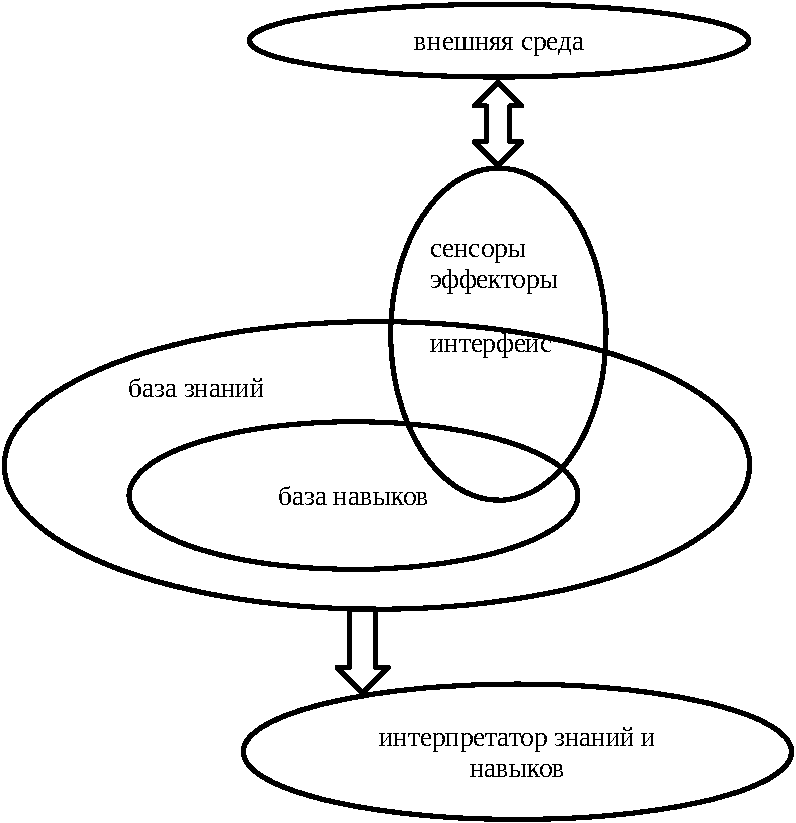
\includegraphics{figures/arch.pdf}\\}
		\bigskip
	\end{scnsubstruct}
\end{SCn}

\scsubsection[
    \protect\scneditor{Банцевич К.А.}
    \protect\scnmonographychapter{Глава 1.2. Интеллектуальные компьютерные системы нового поколения и технология комплексной поддержки их жизненного цикла}
    ]{Предметная область и онтология смыслового представления информации}
\label{sd_sem_inf_rep}
\begin{SCn}
	\scnsectionheader{\currentname}

	\begin{scnsubstruct}

		\scnrelto{частная предметная область и онтология}{Предметная область и
			онтология информационных конструкций}
		\begin{scnhaselementrolelist}{класс объектов исследования}
			\scnitem{смысловое представление информации}
		\end{scnhaselementrolelist}

		\begin{scnhaselementrolelist}{класс объектов исследования}
			\scnitem{семантическая сеть}
				\begin{scnindent}
					\begin{scnsubdividing}
						\scnitem{нерафинированная семантическая сеть}
						\scnitem{рафинированная семантическая сеть}
					\end{scnsubdividing}
					\begin{scnsubdividing}
						\scnitem{абстрактная семантическая сеть}
							\begin{scnindent}
								\scnidtf{семантическая сеть, абстрагирующаяся от того, как
									физически представлены ее элементарные (атомарные) фрагменты, а также связи
									инцидентности между этими фрагментами}
							\end{scnindent}
						\scnitem{графически представленная семантическая сеть}
							\begin{scnindent}
								\scnidtf{нарисованная семантическая сеть}
							\end{scnindent}
						\scnitem{семантическая сеть, хранимая в графодинамической памяти}
							\begin{scnindent}
								\scnrelboth{следует отличать}{представление семантической сети
									в адресной памяти}
								\scnnotsubset{семантическая сеть}
								\scnidtf{представление семантической сети в виде линейной
									информационной конструкции, которая хранится в адресной памяти и которая,
									строго говоря, уже не является семантической сетью, но является информационной
									конструкцией, семантически эквивалентной соответствующей (представляемой)
									семантической сети}
							\end{scnindent}
					\end{scnsubdividing}
				\end{scnindent}
			\scnitem{язык семантических сетей}
				\begin{scnindent}
					\scnidtf{язык, все тексты которого являются семантическими
						сетями}
					\begin{scnsubdividing}
						\scnitem{специализированный язык семантических сетей}
						\scnitem{универсальный язык семантических сетей}
					\end{scnsubdividing}
					\scnsuperset{язык рафинированных семантических сетей}
				\end{scnindent}
		\end{scnhaselementrolelist}

		\begin{scnrelfromvector}{рассматриваемые вопросы}
			\scnfileitem{Что такое семантические сети и в чем их принципиальное
				отличие от других вариантов представления информации}
			\scnfileitem{До какой степени можно минимизировать алфавит элементов
				семантических сетей}
			\scnfileitem{Можно ли все описываемые связи свести к бинарным связям и
				почему это целесообразно}
			\scnfileitem{Можно ли разработать \uline{универсальный} язык
				семантических сетей}
			\scnfileitem{До какой степени можно упростить синтаксические структуры
				семантических сетей до, условно говоря, рафинированного вида}
			\scnfileitem{Какими достоинствами обладает семантические сети}
		\end{scnrelfromvector}

		\begin{scnrelfromlist}{ссылка}
			\scnitem{Понятие Технологии OSTIS}
				\begin{scnindent}
					\scntext{аннотация}{В указанном сегменте \textit{Стандарта
							OSTIS} рассматриваются принципы, лежащие в основе \textit{Технологии OSTIS},
						основным из которых является ориентация на использование
						\textit{\uline{универсального} языка рафинированных семантических сетей} в
						качестве внутреннего языка \textit{интеллектуальных компьютерных систем}}
				\end{scnindent}
			\scnitem{Описание внутреннего языка ostis-систем}
				%\newpage
				\begin{scnindent}
					\scntext{аннотация}{В указанном разделе \textit{Стандарта
						OSTIS} рассматриваются принципы, лежащие в основе \textit{универсального языка
						рафинированных семантических сетей}, используемого в качестве внутреннего языка
						\textit{ostis-систем} -- \textit{интеллектуальных компьютерных систем}
						следующего поколения}
				\end{scnindent}
			\scnitem{Описание языка графического представления знаний ostis-систем}
				\begin{scnindent}
					\scntext{аннотация}{В указанном разделе \textit{Стандарта
						OSTIS} рассматриваются принципы, лежащие в основе универсального языка
						графически представленных семантических сетей, используемого в
						\textit{пользовательском интерфейсе ostis-систем}}
				\end{scnindent}
			\scnitem{\cite{Birukov1960}}
			\scnitem{\cite{Morris2001}}
			\scnitem{\cite{Pirs2009}}
			\scnitem{\cite{Stepanov1971}}
			\scnitem{\cite{MelchukST}}
		\end{scnrelfromlist}

		\bigskip
		\scnheader{знак}
		\scnidtf{фрагмент информационной конструкции, обладающий свойством,
			\uline{обозначать} некоторую сущность (объект), которая наряду с другими
			сущностями описывается указанной информационной конструкцией}
		\scntext{примечание}{\uline{Форма} представления знаков в известной степени
			условна и является результатом соглашения между носителями соответствующего
			языка. Знак может быть, например, представлен:
			\begin{scnitemize}
				\item  в виде фрагмента речевого сообщения (последовательностью
				фонем);
				\item в виде строки символов (последовательности букв) в
				заданном алфавите;
				\item в виде иероглифа, пиктограммы;
				\item в виде жеста.
			\end{scnitemize}}
		\scniselementrole{ключевой знак}{Предметная область и онтология
			информационных конструкций}
			\begin{scnindent}
				\scnhaselement{раздел Базы знаний IMS.ostis}
			\end{scnindent}
		\scntext{характеристика элементов данного множества}{Знаки,
			используемые в различных языках, характеризуются:
			\begin{scnitemize}
				\item синтаксической структурой, по совпадению (изоморфизму)
				которых для разных знаокв предполагается их синонимия;
				\item денотационной семантикой, т.е. той сущностью, которая
				обозначается соответствующим знаком;
				\item типом (классом) обозначаемой сущности, которая может
				быть:
				\begin{scnitemizeii}
					\item материальным(физическим) элементом (точкой)
					абстрактного пространства, множеством, которое может быть:
					\begin{scnitemizeiii}
						\item связью;
						\item классом;
						\item структурой;
					\end{scnitemizeiii}
					\item реальной и вымышленной сущностью;
					\item константной (конкретной) и переменной
					(произвольной) сущностью;
					\item постоянно существующей и временно существующей
					сущностью (прошлой, настоящей, будущей);
				\end{scnitemizeii}
				\item множеством тех связей, которые связывают сущность,
				обозначаемую данным знаком с другими сущностями, а также, если данный знак
				обозначает некоторую связь, множеством сущностей, которые связаны этой связью,
				т.е. сущностей, являющихся компонентом этой связи;
				\item текущим статусом самого знака в памяти кибернетической
				системы, который может быть:
				\begin{scnitemizeii}
					\item логически удаленным знаком;
					\item настоящим знаком;
					\item предлагаемым (возможно, будущим) знаком.
				\end{scnitemizeii}
			\end{scnitemize}}

		\bigskip
		\scnheader{денотат*}
		\scnidtf{денотат заданного знака*}
		\scnidtf{объект, обозначаемый заданным знаком*}
		\scnidtf{денотационная семантика заданного знака*}
		\scnidtf{смысл заданного знака*}
		\scnidtf{Бинарное ориентированное отношение, каждая пара которого
			связывает:
			\begin{scnitemize}
				\item некоторый знак, представленный в той или иной форме в тексте
				исследуемого языка;
				\item \uline{со знаком} той сущности, которая обозначается указанным
				выше знаком в рамках используемого метаязыка.
			\end{scnitemize}}

		\scntext{примечание}{Данное отношение используется, когда с помощью одного
			языка необходимо описать денотационную семантику другого языка. Фактически речь
			идет о переводе заданного знака, входящего в состав некоторого рассматриваемого
			текста, принадлежащего некоторому исследуемому языку (языку-объекту), на
			некоторый метаязык (в нашем случае на SC-код), денотационная семантика которого
			нам считается априори известной. Указанный перевод есть связь заданного знака с
			синонимичным ему знаком, входящим в состав текста, принадлежащего указанному
			метаязыку.}
		\scnrelboth{обратное отношение}{внешний sc-идентификатор*}
			\begin{scnindent}
				\scnidtf{быть знаком, обозначающим заданную сущность*}
			\end{scnindent}
		% \scniselementlist{ключевой знак}{Описание внешних идентификаторов знаков, входящих в тексты внутреннего языка ostis-систем\\

		% \scniselement{раздел Базы знаний IMS.ostis}
		% Предметная область и онтология знаков, входящих в тексты внутреннего языка ostis-систем\\
		% \scniselement{раздел Базы знаний IMS.ostis}}

		\scnheader{информационная конструкция}
		\scnidtf{информация}
		\scntext{примечание}{В общем случае информационная конструкция представляет
			собой сложную иерархическую структуру, каждому уровню иерархии которой
			соответствует определенный класс информационных конструкций.}
		\scnsuperset{синтаксически элементарный фрагмент информационной конструкции}
			\begin{scnindent}
				\scnidtf{атомарный фрагмент информационной конструкции}
				\scnidtf{элемент информационной конструкции}
				\scntext{примечание}{Примерами таких элементарных фрагментов информационных
					конструкций являются буквы}
				\scnsuperset{буква}
			\end{scnindent}
		\scnsuperset{простой знак}
			\begin{scnindent}
				\scnidtf{семантически элементарный фрагмент информационной конструкции}
				\scnsubset{знак}
			\end{scnindent}
		\scnsuperset{выражение}
			\begin{scnindent}
				\scnidtf{сложный (непростой) знак}
				\scnidtf{знак, являющийся одновременно некоторым знанием обозначаемой
					сущности (спецификацией этой сущности)}
				\scnidtf{знак, построенный как выражение вида тот, который... }
				\scnidtf{знак, в состав которого входят другие знаки}
				\scnsubset{знак}
			\end{scnindent}
		\scnsuperset{простой текст}
			\begin{scnindent}
				\scnidtf{минимальная синтаксически целостная и корректная (правильная)
					информационная конструкция, включающая в себя:
					\begin{scnitemize}
						\item знак некоторой описываемой связи;
						\item минимальную спецификацию указанного знака связи (указание
						отношения, которому это связь принадлежит);
						\item указание \uline{всех} компонентов описываемой связи (знаков всех
						сущностей, связываемых этой связью, и/или всех знаков, связываемых этой связью
						-- описываемая связь может связывать не только внешние	описываемые сущности,
						но и сами знаки);
						\item если описываемая связь не является бинарной, то связи с её
						компонентами могут потребовать явного представления знаков этих связей с
						дополнительным указанием роли этих компонентов.
					\end{scnitemize}}
				\scnsubset{текст}
			\end{scnindent}
		\scnsuperset{сложный текст}
			\begin{scnindent}
				\scnidtf{информационная конструкция, являющаяся результатом соединения
					нескольких простых текстов}
				\scnsubset{текст}
			\end{scnindent}
		\scnsuperset{простое знание}
			\begin{scnindent}
				\scnidtf{минимальная семантические целостная информационная конструкция}
				\scnidtf{знание, в состав которого не входят другие знания}
				\scnsubset{знание}
			\end{scnindent}
		\scnsuperset{сложное знание}
			\begin{scnindent}
				\scnidtf{информационная конструкция, являющаяся результатом соединения
					нескольких простых знаний}
				\scnidtf{знание, в состав которого не входят другие знания}
				\scnsubset{знание}
			\end{scnindent}
		\scniselementrole{ключевой знак}{Предметная область и онтология информационных конструкций}

		\bigskip\scnheader{смысловое представление информации}
		\scnidtf{смысловая форма представления информации}
		\scnidtf{смысловое представление информационной конструкции}
		\scnidtf{знаковая конструкция (текст), представленная в смысловой
			форме}
		\scnidtf{смысловое представление информационной конструкции}
		\scnidtftext{часто используемый sc-идентификатор}{смысл}
		\scnidtf{смысловое представление}
		\scnidtf{семантическое представление информации}
		\scntext{основной принцип}{Как можно меньше лишнего, не имеющего
			отношения к смыслу представляемой информации.}
		\scnidtf{такое представление информационной конструкции, которое
			существенно упрощает соответствие между структурой самой этой информационной
			конструкции и описываемой (отображаемой) ею конфигурацией связей между
			рассматриваемыми (исследуемыми) сущностями}
		\scnidtf{смысловое представление знаковой конструкции}
		\scnidtf{абстрактная знаковая конструкция, являющаяся
			\uline{инвариантом} соответствующего максимального класса семантически
			эквивалентных знаковых конструкций}
		\scnidtf{смысл информационной конструкции}
		\scnidtf{денотационная семантика информационной конструкции}
		\scnidtf{смысловое представление информационной конструкции}
		\scntext{примечание}{Суть (смысл, денотационная семантика) любой
			информационной конструкции (информационной модели) сводится к описанию системы
			(конфигурации) связей между списываемыми (рассматриваемыми) сущностями. Важно,
			чтобы эта суть не была \uline{закамуфлирована} различными синтаксическими
			деталями, не имеющими никакого отношения к указанному смыслу (синтаксическая
			структура знаков, многократное повторение одного и того же знака, синонимия,
			омонимия, местоимения, предлоги, знаки препинания, разделители, ограничители,
			падежи и т.п.) а обусловленными \uline{формой} представления информационных
			конструкций, например, их линейностью.}
		\scntext{пояснение}{Смысловое представление любой информации в
			конечном счете сводится:
			\begin{scnitemize}
				\item{к перечню знаков конкретных описываемых сущностей - как первичных
				            сущностей, так и вторичных сущностей, которые сами являются информационными
				            конструкциями (фрагментами данной конструкции)};
				\item{к явному описанию связи между знаками вторичных сущностей и
				            самими этими сущностями (т.е. фрагментами информационной конструкции)};
				\item{к описанию других связей между описываемыми сущностями}
			\end{scnitemize}
			\vspace{-0.6\baselineskip}}
		\newpage
		\scntext{пояснение}{Формализация смысла представляемой информации,
			т.е. строгое уточнение того, что такое \textit{смысловое представление
				информации}, является объективной основой для \uline{унификации} представления
			информации в \textit{памяти компьютерных систем} и \uline{ключом} к решению
			многих проблем семантической совместимости и эволюции компьютерных систем и
			технологий.
			
			Согласно \textit{Мартынову В. В.} (\cite{Martynov}), <<фактически
			всякая мыслительная деятельность человека (не только научная), как полагают
			многие ученые, использует \uline{внутренний семантический код}, на который
			переводят с естественного языка и с которого переводят на естественный язык.
			Поразительная способность человека к идентификации огромного множества
			структурно различных фраз с одинаковым \textit{смыслом} и способность
			\uline{запомнить смысл вне этих фраз} убеждает нас в этом.>>
			
			Приведем также слова \textit{Мельчука И. А.} (\cite{MelchukST}):
			
			<<Идея была следующая -- язык надо описывать следующим образом: надо уметь записывать смыслы фраз. \uline{Не
			фразы, а их \textit{смыслы}}, что отдельно. Плюс построить систему, которая по
			смыслу строит фразу. Это та область или тот поворот исследований, при котором
			интуиция способного лингвиста работает лучше всего: как выразить на данном
			языке данный смысл. Это -- то, для чего лингвистов учат.
			
			Лингвистический	\textit{смысл} научного текста -- это совсем не то, что ты, читая его, из него
			извлекаешь. Это, очень грубо говоря, инвариант синонимических перифраз. Ты
			можешь один и тот же смысл выразить очень многими способами. Когда ты говоришь,
			то можешь сказать по-разному: \scnqqi{Сейчас я налью тебе вина}, или: \scnqqi{Дай, я тебе
			предложу вина}, или: \scnqqi{Не выпить ли нам по бокалу?}, -- все это имеет один и тот
			же смысл. И вот можно придумать, как записывать этот \textit{смысл}. Именно
			его. Не фразу, а \textit{смысл}. И работать надо от этого \textit{смысла} к
			реальным фразам. Синтаксис там по дороге тоже нужен, но он нужен именно по
			дороге, он не может быть ни конечной целью, ни начальной точкой. Это --
			промежуточное дело.>> (\cite{Melchuk}).}
		\scntext{примечание}{Грамотная унификация (стандартизация) \textit{смыслового
				представления информации} не должна привести к ограничению творческой свободы
			авторов различного вида публикуемых научно-технических знаний (и, в том числе,
			разработчиков \textit{баз знаний}), не должна гарантировать
			\textit{семантическую совместимость} различных \textit{знаний}, представленных
			различными авторами (разумеется, при условии соблюдения соответствующих правил
			построения этих \textit{знаний}). При этом любые \textit{стандарты} (в том
			числе и принятые стандарты \textit{смыслового представления информации}) должны
			постоянно эволюционировать. Текущая версия любого стандарта должна быть не
			догмой, а точкой опоры для дальнейшего совершенствования этого стандарта.}
		\scnsuperset{УСК}
			\begin{scnindent}
				\scnidtf{Универсальный Семантический Код}
				\scnrelfrom{автор}{Мартынов В. В.}
				\scntext{примечание}{Разработанный Мартыновым В. В. Универсальный
					Семантический Код стал важнейшим этапом создания универсальных формальных
					средств смыслового представления знаний. Основная методологическая идея
					\textit{Мартынова В. В.}, касающаяся построения \textit{языка смыслового
					представления знаний}, заключается в том, чтобы выделить смысловые кирпичики ,
					имеющие достаточно общий характер, а многообразие конкретных смыслов
					конструировать комбинаторно за счёт различных комбинаций (конфигураций) из этих
					кирпичей. Это можно назвать принципом минимизации типов атомарных смысловых
					фрагментов.}
				\scnrelto{ключевой знак}{\cite{Martynov1984}}
			\end{scnindent}

		\scnheader{смысловое представление информации*}
		\scnidtftext{пояснение}{\textit{Бинарное ориентированное отношение},
			каждая \textit{пара} которого связывает некоторую \textit{информационную
				конструкцию} со смысловым представлением этой \textit{информационной
				конструкции*}.}
		\scnsubset{формализация*}
		\bigskip
		
		\scnheader{формализация*}
		\scniselement{бинарное ориентированное отношение}
		\scnidtf{формализация информации*}
		\scnidtf{пара, связывающая менее формализованное и более
			формализованное представление некоторой информации*}
		\scnidtf{формализация информационной модели некоторой описываемой
			(моделируемой) системы взаимосвязанных сущностей*}
		\scnidtf{Бинарное ориентированное отношение, каждая \textit{пара}
			которого, связывает два \textit{семантически эквивалентных} знания, второе из
			которых является более точным (более точно сформированным) знанием по сравнению
			с первым \textit{знанием}*.}
		\scntext{пояснение}{Повышение точности (строгости) формулировки
			знания -- минимизация (а в идеале -- исключение) \uline{неоднозначной}
			семантической интерпретации этой формулировки, т.е. несоответствия того, что
			хотел сказать  автор формулировки, и того, как его поняли. Формализация знаний
			предполагает (1) точное (строгое) описание \textit{синтаксиса и денотационной
				семантики} того \textit{языка}, на котором формулируются \textit{знания} и (2)
			максимально возможное \uline{упрощение} синтаксических и семантических
			принципов, лежащих в основе указанного \textit{языка}. Очевидно, что
			\textit{естественные языки} указанным требованиям не удовлетворяют и,
			следовательно, не могут быть основой для точной формулировки
			\textit{научно-технических знаний} и, соответственно, для представления этих
			\textit{знаний} в \textit{памяти интеллектуальных компьютерных систем}.
			Очевидно также, что разработка \textit{\uline{универсального} языка}
			формального представления научно-технических знаний является \uline{основой}
			для глубокой конвергенции различных научно-технических дисциплин, для
			расширения областей применения современной математики и даже для появления
			новых разделов математики, которые, например, изучают общие свойства
			\textit{универсального смыслового пространства} и, в частности, свойство
			семантического расстояния(семантической близости) как между различными
			\textit{знаками}, так и между различными \textit{знаковыми конструкциями}
			(конфигурациями знаков).}
			\begin{scnindent}
				\scntext{примечание}{Слово математика  означает точное знание .}
					\begin{scnindent}
						\scnrelto{цитата}{\cite{Arnold2012}}
					\end{scnindent}
			\end{scnindent}
		\scntext{примечание}{Формализация информационной модели есть не что иное как
			движение  в сторону семантического (смыслового) представления этой модель, т.е.
			переход к такому представлению этой модели, в котором мы избавляемся от всего,
			не имеющего отношения к сути моделируемой системы и касающегося только способа
			построения этой модели (т.е. её синтаксической структуры). }
		\scntext{примечание}{Нет проблемы записать любое \textit{знание} в
			компьютерную \textit{память}. Для этого надо придумать соответствующий формат
			их кодирования. Но есть проблема представить это \textit{знание} так, чтобы с
			ним было легко работать, чтобы с использованием этого \textit{знания} можно
			было достаточно удобно (без лишних накладных расходов, обусловленных выбранным
			способом представления) решать самые различные информационные \textit{задачи}
			(задачи интеграции знаний, информационного поиска по базе знаний, верификации и
			оптимизации баз знаний, логического вывода, поиска способов решения задач,
			хранимых в базе знаний и т. д.).Какими характеристиками должно обладать удобное
			представление знаний, удовлетворяющее указанным требованиям. Очевидно, что
			такое представление есть не что иное, как формальная (математическая) модель,
			семантически эквивалентная этим знаниям. Т.е. удобно представить знание -- это
			фактически построить соответствующую этому знанию \textit{математическую
				модель}.Для интеллектуальных компьютерных систем важно не просто приобрести
			знания, но и представить их в такой форме, которая была бы удобна не только для
			человека (пользователя и разработчика), но и для различных компьютерных систем,
			т.е. не требовала бы переоформление (перезаписи) этих знаний для различных
			компьютерных систем. Очевидно, что такая форма записи (представления) знаний
			должна быть абсолютно не зависящий от различных компьютерных платформ.Это и
			есть главная цель формализации знаний, обеспечивающей эффективную автоматизацию
			обработки этих знаний.}

		\scnheader{формальное представление информации}
		\scnsubset{информация}
			\begin{scnindent}
				\scnidtf{информационная конструкция}
			\end{scnindent}
		\scntext{вопрос}{Почему разработка и использование формальных моделей
			(математических моделей) представления \textit{информации} является важнейшим
			этапом развития любой научной и научно-технической дисциплины.}
		\begin{scnindent}
			\begin{scnrelfromset}{ответ}
				\scnfileitem{Формализация любой \textit{предметной области} даёт
					возможность более конструктивно накапливать, интегрировать, понимать и
					систематизировать новые \textit{знания} об этой \textit{предметной области}}
				\scnfileitem{Формализация \textit{предметной области} обеспечивает
					более строгую верификацию, обоснование (аргументацию, доказательство) и
					согласование различных точек зрения}
				% \newpage
				\scnfileitem{Формализация \textit{предметной области} создает условия
					для разработки строгих и легко воспроизводимых (реализуемых) \textit{методов}
					решения различных \textit{классов задач}}
			\end{scnrelfromset}
		\end{scnindent}
		\scnrelto{достоинства}{формальное представление информации}
		\scnidtf{формальное (формализованное) представление информационной
			конструкции}
		\scnsubset{смысловое представления информации}
		\scntext{примечание}{Высшим уровнем качества \textit{формального
				представления информации} является смысловое представление этой информации}
		\scnidtf{формальная модель системы описываемых взаимосвязанных
			сущностей}
		\scnidtf{математическая модель системы описываемых взаимосвязанных
			сущностей}
		\scnidtf{формула}
		\scntext{примечание}{Сам термин \scnqqi{\textit{формальное представление
				информации}} свидетельствует о том, что при таком представлении
			\textit{информации} сама \uline{форма} представляемой информационной
			конструкции (т.е. синтаксическая структура этой конструкции) имеет очевидную
			аналогию с описываемой конфигурацией связей между соответствующими
			соответствующими описываемыми \textit{сущностями}.В предельном идеальном
			случае указанная аналогия между формой и смыслом информационной конструкции
			должна быть изоморфизмом.}
		\scntext{примечание}{Формализация формализации рознь и, соответственно,
			степень приближения формы представления информации к идеальному  смысловому
			представлению может быть различной. Разработка такого идеального  \textit{языка
				смыслового представления информации} должна руководствоваться следующими
			основными критериями:
			\begin{scnitemize}
				\item максимально возможное упрощения синтаксиса (как можно меньше
				синтаксических излишеств и синтаксического разнообразия);
				\item обеспечение \uline{универсальности} языка.
			\end{scnitemize}
			Подчеркнем, что обеспечение универсальности \textit{языка смыслового
				представления информации} является весьма нетривиальной задачей, т.к. сложно
			одновременно достигнуть две противоречащие друг другу цели- обеспечить простоту
			синтаксиса языка и его неограниченную семантическую мощность. Косвенным
			подтверждением этого является большое количество созданных человечеством
			специализированных \textit{формальных языков}, \textit{языков смыслового
				представления информации} и даже \textit{языков семантических сетей}, что
			свидетельствует о востребованности \textit{смыслового представления
				информации}.}
		\begin{scnsubdividing}
			\scnitem{формальное представление информации, не являющееся смысловым}
			\scnitem{смысловое представление информации, не являющееся
				семантической сетью}
			\scnitem{нерафинированная семантическая сеть}
				\begin{scnindent}
					\scnidtf{смысловое представления информации 2-го уровня}
				\end{scnindent}
			\scnitem{рафинированная семантическая сеть}
				\begin{scnindent}
					\scnidtf{смысловое представление информации 3-го уровня}
				\end{scnindent}
		\end{scnsubdividing}

		\bigskip
		\scnheader{смысловое представление информации, не являющееся семантической сетью}
		\scntext{примечание}{Данному уровню смыслового представления информации
			соответствуют предлагаемые нами универсальные формальные языки SCs-код и SCn-код}
		\scnsuperset{SCs-код}
			\begin{scnindent}
				\scniselement{универсальный формальный язык}
				\scniselementrole{ключевой знак}{Описание языка линейного представления знаний ostis-систем}
			\end{scnindent}
		\scnsuperset{SCn-код}
		\begin{scnindent}
			\scniselement{универсальный формальный язык}
			\scniselementrole{ключевой знак}{Описание языка структурированного представления знаний ostis-систем}
		\end{scnindent}
		\begin{scnreltovector}{принципы, лежащие в основе}
			\scnfileitem{В состав \textit{смыслового представления информации, не
				являющегося семантической сетью} могут входить все уровни иерархии
				представления информационной конструкции --
				\begin{scnitemize}
					\item синтаксически элементарные фрагменты информационной конструкции,
					из которых строятся простые знаки описываемых сущностей, а также разделители и
					ограничители
					\item простые знаки
					\item выражения
					\item простые тексты
					\item сложные тексты
					\item простые знания
					\item сложные знания.
				\end{scnitemize}}

			\scnfileitem{Множество всех описываемых сущностей, \uline{не являющихся
					связями}, разбивается на два подмножества:
				\begin{scnitemize}
					\item каждой сущности, принадлежащей первому подмножеству,
					\uline{взаимно однозначно} соответствует множество \uline{синтаксически
						эквивалентных} (синтаксически одинаковых) \textit{простых знаков}, каждый из
					которых обозначает указанную сущность
					\item каждой сущности, принадлежащей второму подмножеству,
					соответствует в общем случае \uline{семейство} множеств, кажо из которых
					является максимальным множеством синтаксически эквивалентных выражений,
					обозначающих указанную сущность.
				\end{scnitemize}}
				\newline
				\begin{scnindent}
					\scntext{следовательно}{Здесь синонимия \textit{простых знаков},
						имеющих \uline{разную} синтаксическую структуру, отсутствует, а вот синонимия
						\textit{выражений}, имеющих разную синтаксическую структуру, вполне возможна.
						Подчеркнем при этом, что в рамках \textit{смыслового представления информации,
							не являющегося семантической сетью},
						% \bigspace
						\textit{знаки} (как \textit{простые знаки}, так и \textit{выражения}),
						имеющие одинаковую синтаксическую структуру, считаются также и семантически
						эквивалентными, т.е. обозначающими одну и ту же сущность. Это означает
						отсутствие омонимии синтаксически эквивалентных знаков.}
					\scntext{следовательно}{В рамках \textit{смыслового представления
							информации, не являющегося семантической сетью}, простые знаки, обозначающие
						\uline{разные} сущности, имеют легко устанавливаемое отличие своих
						синтаксических структур, а простые знаки, обозначающие одну и ту же сущность
						имеют легко устанавливаемое сходство своих синтаксических структур. Таким
						образом, в рамках \textit{смыслового представления информации, не являющегося
							семантической сетью},
						% \bigspace
						\uline{дублирование знаков}, т.е. многократное вхождение
						\textit{знаков} одной и той же сущности, \uline{допускается}.}
				\end{scnindent}
			\scnfileitem{Связи как вид описываемых сущностей имеют очень важные
				особенности:
				\begin{scnitemize}
					\item каждой описываемой \textit{связи} \uline{однозначно}, а в
					подавляющем числе случаев и \uline{взаимно однозначно} соответствует
					\textit{простой текст}, являющийся контекстом (спецификацией) этой
					\textit{связи}
					\item весьма редки \textit{кратные связи}, т.е. \textit{свзяи},
					принадлежащие одному и тому же \textit{отношению} и связывающие одинаковым
					образом одни и те же \textit{сущности}
					\item довольно редко \textit{связи} являются компонентами других
					\textit{связей}.
				\end{scnitemize}}
				\begin{scnindent}
					\scntext{следовательно}{Для подавляющего числа описываемых
						\textit{связей} нет никакой необходимости вводить обозначающие их
						\textit{знаки}, если эти \textit{связи} описываются соответствующими
						\textit{простыми текстами}. Вместо таких \textit{знаков} можно ввести условные
						представления этих \textit{связей}, отражающие их вид и направленность. Такие
						условные представления (изображения) описываемых \textit{связей} можно считать
						\textit{знаками}, но \textit{знаками}, семантические свойства которых
						принципиально отличаются от тех \textit{знаков} описываемых \textit{сущностей},
						которые мы рассматривали выше. Любые данного вида разные \textit{знаки}
						описываемых \textit{связей} даже, если, они являются \textit{синтаксически
							эквивалентными}, т.е. имеют одинаковую структуру, считаются \textit{знаками}
						\uline{разных} описываемых \textit{связей}. Синонимия таких \textit{знаков}
						принципиально возможна, но только в том случае, если \textit{простые тексты},
						описывающие соответствующие \textit{связи}, будут полностью
						\uline{продублированы}.}
				\end{scnindent}
			\scnfileitem{Для описания связей между описываемыми сущностями в
				смысловом представлении информации нет необходимости использовать такие приемы
				естественных языков, как склонения, спряжения, семантическая значимость
				последовательности знаков.}
			\scnfileitem{В случае, если с помощью \textit{простых текстов}
				необходимо описать контекст (спецификацию) нескольких \uline{кратных}
				\textit{связей}, все эти \textit{связи} необходимо обозначить \textit{знаками}
				первого типа -- знаками, \textit{синтаксическая структура} каждого из которых
				\uline{уникальна.}Кроме этого, необходимо ввести знак, который обозначает
				\textit{связь инцидентности} между описываемой \textit{связью} и компонентом
				этой \textit{связи}, и который относится к числу \textit{знаков} второго типа
				-- \textit{знаков}, разные экземпляры (разные вхождения) которого считаются
				обозначениями \uline{разных} \textit{связей}}
			\scnfileitem{Для явного указания синонимии двух разных \textit{знаков}
				первого типа, имеющих разную \textit{синтаксическую структуру}, вводится
				фиктивная \textit{связь равенства}, которая сама не является описываемой
				\textit{связью}, а только указывает факт синонимии двух \textit{знаков}, по
				крайней мере один из которых должен быть \textit{выражением}.}
			\scnfileitem{Каждая описываемая \textit{сущность} должна быть
				специфицирована путем указания типа этой \textit{сущности}. Описываемая
				\textit{сущность} может быть:
				\begin{scnitemize}
					\item \textit{материальной сущностью}
					\item \textit{точкой абстрактного пространства}
					\item {\textit{множеством}:
					            \begin{scnitemizeii}
						            \item \textit{связью}
						            \item \textit{классом}
						            \item \textit{структурой}
					            \end{scnitemizeii}
					      }
					\item \textit{реальной сущностью}
					\item \textit{вымышленной сущностью}
					\item \textit{константой}
					\item \textit{переменной}
					\item \textit{постоянной сущностью}
					\item{\textit{временной сущностью}:
					            \begin{scnitemizeii}
						            \item \textit{прошлой сущностью}
						            \item \textit{настоящей сущностью}
						            \item \textit{будующей сущностью}.
					            \end{scnitemizeii}
					      }
				\end{scnitemize}
				Кроме того, сам \textit{знак} описываемой сущности может иметь
				следующий статус:
				\begin{scnitemize}
					\item{\textit{логически удаленный знак}}
					\item{\textit{настоящий знак}}
					\item{\textit{будущий знак}.}
				\end{scnitemize}
			}
			\scnfileitem{Возможно дублирование информации, т.е. могут
				присутствовать семантически эквивалентные информационные конструкции, входящие
				в остав одной информационной конструкции (например, в состав информации,
				хранимой в памяти одной компьютерной системы). Но при этом есть принципиальная
				возможность обнаружить такое дублирование информации.}
		\end{scnreltovector}

		\bigskip
		\scnheader{графовая структура}
		\scnidtftext{определение}{абстрактная (математическая) структура, которая задается:
			\begin{scnitemize}
				\item {множеством ее элементов:
				            \begin{scnitemizeii}
					            \item множеством ее вершин (узлов);
					            \item {множеством ее связок:
					                        \begin{scnitemizeiii}
						                        \item множеством ее ребер (неориентированных пар
						                        элементов графовой структуры);
						                        \item множеством ее дуг (ориентированных пар элементов
						                        графовой структуры);
						                        \item множеством ее гиперребер, каждое из которых
						                        является конечным множеством элементов графовой структуры, имеющим мощность
						                        больше двух
					                        \end{scnitemizeiii}}
				            \end{scnitemizeii}}
				\item бинарным ориентированным отношением инцидентности, связывающим
				каждую связку графовой структуры с каждым компонентом (элементом) этой связки.
			\end{scnitemize}
		}
		\newpage
		\scnheader{следует отличать*}
		\begin{scnhaselementset}
			\scnfileitem{\textit{графовую структуру} как абстрактный математический
				объект, в рамках которого не уточняется то, как выглядят (представляются,
				изображаются) элементы графовой структуры и связи их инцидентности}
			\scnfileitem{представление (изображение) \textit{графовой структуры} --
				ее рисунок, ее представление в компьютерной памяти в виде матрицы
				инцидентности, матрицы смежности, списковой структуры}
		\end{scnhaselementset}

		\scnheader{графовая структура}
		\scnidtftext{часто используемый sc-идентификатор}{дискретная
			информационная конструкция}
		\scntext{примечание}{Поскольку любая \textit{графовая структура} является
			дискретной математической моделью, которая может описывать любое множество
			\textit{сущностей}, связанных между собой заданным множеством \textit{связей},
			все \textit{графовые структуры} с полным основанием можно считать дискретными
			\textit{информационными конструкциями}. Более того, любая дискретная
			\textit{информационная конструкция} (в том числе, и обычная цепочка символов) с
			формальной точки зрения является \textit{графовой структурой}. Тот факт, что
			теория графов рассматривает синтаксические  свойства \textit{графовых структур}
			с точностью до их изоморфизма, не лишает \textit{графовые структуры}
			соответствующих семантических  свойств.}
		\scntext{пояснение}{С семантической точки зрения графовая структура
			-- это нелинейная (в общем случае) знаковая конструкция, в состав которой могут
			входить знаки \uline{любых} сущностей. При этом указанные знаки
			\uline{синтаксически} разбиваются на два класса --
			\begin{scnitemize}
				\item на \textit{знаки} сущностей, которые не являются \uline{связями}
				между сущностями -- в теории графов такие знаки называются узлами (вершинами);
				\item на знаки \uline{связей} между \textit{сущностями} -- к таким
				\textit{знакам} относятся ребра неориентированных графов, гиперребра
				гиперграфов, дуги ориентированных графов.
			\end{scnitemize}
			Кроме того, на множестве знаков \textit{сущностей}, входящих в состав
			\textit{графовой структуры}, задаются \textit{отношения инцидентности}, которые
			связывают \textit{знаки} связей, входящих  в состав \textit{графовой
			структуры}, со знаками тех \textit{сущностей} которые являются компонентами
			указанных \textit{связей}.
			
			Теория графов рассматривает только синтаксические
			аспекты \textit{графовых структур}.Семантика \textit{графовой структуры}
			задается \textit{онтологией}, специфицирующей систему понятий, экземплярами
			которых являются элементы этой графовой структуры, т.е. \textit{знаки},
			входящие в состав этой \textit{графовой структуры}.}

		\scnheader{семантическая сеть}
		\scnidtf{\textit{графовая структура}, являющаяся \uline{формальным
				уточнением} одного из видов \textit{смыслового представления информации}}
		\scnsubset{графовая структура}
		\scnsubset{смысловое представление информации}
		\begin{scnindent}
			\scnsubset{знаковая структура}
		\end{scnindent}
		\scnidtf{графовая структура, \uline{вершины} (узлы) которой трактуются
			как знаки некоторых описываемых сущностей, а \uline{связки} (ребра, дуги,
			гиперребра, гипердуги) которой трактуются как знаки связей между описываемыми
			сущностями и/или знаками этих сущностей}
		\scnidtf{\uline{абстрактная} графовая и в общем случае нелинейная
			знаковая конструкция (знаковая структура), являющаяся вариантом
			\uline{смыслового} представления соответствующей информации}
		\scnidtftext{explanation}{информационная конструкция, в которой
			\uline{явно} выделены знаки \uline{всех} описываемых сущностей, а также знаки
			связей, которые также считаются описываемыми сущностями и которые связывают
			либо сами описываемые сущности, либо описываемые сущности со знаками других
			описываемых сущностей, либо знаки описываемых сущностей}
		\scntext{примечание}{Теоретико-графовая трактовка (уточнение)
			\textit{смыслового представления информации} является вполне естественной, т.к.
			любая описываемая сущность может иметь неограниченное количество связей с
			другими описываемыми сущностями, и очень часто анализ свойств какой-либо
			описываемой сущности предполагает анализ всех представленных (описанных) связей
			этой сущности с различными другими сущностями. Более того, для любых
			описываемых сущностей существует связывающая их связь (все в Мире
			взаимосвязано). Вопрос в том, какая это связь и нужно ли ее описывать. Далеко
			не все то, что можно описывать, целесообразно описывать.}
		\begin{scnrelfromvector}{общие предпосылки}
			\scnfileitem{Информация в знаковой конструкции содержится не в самих
				знаках, а в конфигурации связей между знаками, обозначающими описываемые
				сущности}
			\scnfileitem{Конфигурация связей между описываемыми сущностями \uline{в
					общем случае} \uline{не} являются линейной}
			\scnfileitem{Идеальным \textit{смысловым представлением информации}
				следует считать такую знаковую конструкцию, синтаксическая конфигурация связей
				между знаками которой \uline{изоморфна} конфигурации связей между описываемыми
				сущностями}
		\end{scnrelfromvector}

		\scntext{примечание}{Понятие семантической сети является основным понятием
			для \textit{Технологии OSTIS}. Ранее семантические сети рассматривались не как
			основа технологии разработки интеллектуальных компьютерных систем, а как
			наглядная иллюстрация представления знаний, не имеющая практической перспективы
			из-за сложности реализации, не обладающая универсализмом.Для нас семантические
			сети -- это
			\begin{scnitemize}
				\item формальный подход к построению знаковых конструкций;
				\item формальный подход, позволяющий создавать целое \uline{семейство}
				языков и в том числе языков \uline{универсальных};
				\item основа организации памяти нового типа -- структурно
				перестраиваемой (реконфигурируемой) памяти, обработка информации в которой
				сводится к реконфигурации связей между ее элементами.
			\end{scnitemize}}
		\begin{scnrelfromlist}{достоинства}
			\scnfileitem{\textit{Семантическая сеть} наряду с системами правил
				является весьма распространенным способом представления знаний в
				интеллектуальных системах. Особое значение этот способ представления знаний
				приобретает в связи с развитием сети интернет. Кроме ряда особенностей,
				позволяющих применять семантические сети в тех случаях, когда системы правил не
				применимы, \textit{семантические сети} обладают следующим важным свойством: они
				дают возможность \uline{соединения в одном представлении синтаксиса и
					семантики} или синтаксического и семантического аспектов описаний знаний
				предметной области. Происходит это благодаря тому, что в семантических сетях
				наряду с переменными для обозначения тех или иных объектов (элементов множеств,
				некоторых конструкций из них) присутствуют и сами эти элементы и конструкции присутствуют и связи, сопоставляющие тем или иным переменным
				множества допустимых интерпретаций. Эти обстоятельства позволяют во многих
				случаях резко \uline{уменьшить реальную вычислительную сложность решаемых
					задач}.
				\newline Помимо изобразительных возможностей, семантические сети
				обладают более серьезными достоинствами. То обстоятельство, что \uline{вся
					информация об индивиде} представлена в единственном месте -- в одной вершине --
				означает, что вся эта информация непосредственно доступна в этой вершине, что,
				в свою очередь, \uline{сокращает время поиска}, в частности, при выполнении
				унификации и подстановки в задачах логического вывода.Существует еще одна,
				более тонкая особенность расширенных семантических сетей -- они позволяют
				интегрировать в одном представлении \textit{синтаксис} и \textit{семантику}
				(т.е. интерпретацию) клаузальных форм. Это позволяет в процессе вывода
				обеспечивать взаимодействие синтаксических и семантических, теоретико-модельных
				подходов, что, в свою очередь, также является фактором, зачастую делающим вывод
				практически более эффективным}
				\begin{scnindent}
				\scnrelto{цитата}{Осипов.Г.С.МетодыИИ-2015кн,с.43-54}
					\begin{scnindent}	
						\scnrelto{часть}{\cite{Osipov2015}}
					\end{scnindent}
				\end{scnindent}
			\scnfileitem{Все связи между \textit{знаками}, входящими в состав
				\textit{семантической сети} представляются с помощью специальных связующих
				элементов \textit{семантической сети} (дуг, ребер) и, следовательно, для
				описания указанных связей в \textit{семантической сети} нет необходимости
				использовать такие средства, как предлоги, союзы, падежи, склонения, спряжения,
				различные разделители и ограничители, что существенно упрощает обработку
				\textit{знаний}.}
			\scnfileitem{Соединение синтаксических и семантических аспектов в
				\textit{семантической сети} проявляется в том, что дуга или ребро,
				синтаксически  соединяющая элементы \textit{семантической сети} описывает
				наличие соответствующей \textit{связи} между \textit{сущностями}, обозначаемыми
				указанными элементами \textit{семантической сети}.}
		\end{scnrelfromlist}

		\bigskip
		\scnheader{нерафинированная семантическая сеть}
		\scntext{примечание}{Переход от смыслового представления информации, не
			являющегося семантической сетью, к нерафинированным семантическим сетям
			представляет собой переход к информационным конструкциям, имеющим более простую
			синтаксическую структуру и денотационную семантику.\\\newlineК нерафинированным
			семантическим сетям можно отнести тексты предлагаемого нами универсального
			формального SCg-кода, а также используемые в Semantic Web
			rdf-графы}	
		\scnsuperset{SCg-код}
			\begin{scnindent}
				\scnhaselement{универсальный формальный язык}
				\scnhaselementrole{ключевой знак}{Описание языка графического представления знаний ostis-систем}
			\end{scnindent}
		\scnsuperset{rdf-граф}
		\begin{scnreltovector}{принципы, лежащие в основе}
			\scnfileitem{Поскольку в \textit{информационной конструкции} информация
				содержится не в самих \textit{знаках} (если не считать \textit{знаки},
				являющиеся \textit{выражениями}), а в конфигурации связей между
				\textit{знаками}, очень важно \uline{явно} формально представить саму эту
				конфигурацию \textit{знаков}. И как нельзя лучше для этого подходит понятие
				\textit{графовой структуры} и, соответственно, понятие \textit{семантической
					сети}.\\Что касается \textit{выражений}, то каждое из них легко
				трансформируется в \textit{семантически эквивалентную} информационную
				конструкцию, не являющиюся \textit{выражением}. Заметим, что \textit{выражения}
				используются исключительно для минимизации числа вводимых \textit{знаков}
				(имен) с уникальной синтаксической структурой.}
			\scnfileitem{\uline{Все} элементы, входящие в состав нерафинированной
				семантической сети и представленные узлами, ребрами или дугами, являются
				\textit{знаками}, обозначающими соответствующие описываемые \textit{сущности},
				причём \textit{знаками} второго типа, которые, обозначая соответствующую
				\textit{сущность}, входят в \textit{информационную конструкцию}
				\uline{однократно} (отсутствует многократное вхождение \textit{знаков},
				обозначающих одну и ту же \textit{сущность}). Также \textit{знаки} могут иметь
				синтаксическую структуру, которая не является уникальной для обозначаемой
				\textit{сущности}, а отражает только принадлежность этой сущности к
				соответствующих классам.Таким образом, в \textit{нерафинированной семантической
					сети} в отличие от \textit{смыслового представления информации не являющегося
					семантической сетью}, доминируют не \textit{знаки} первого типа, а
				\textit{знаки} второго типа, которыми в \textit{нерафинированной семантической
					сети} представлены (обозначены) \uline{все} описываемые \textit{сущности}, а в
				\textit{смысловом представлении информации, не являющемся семанитеской сетью},
				представлены \uline{только} \textit{бинарные связи} \uline{и то не все}.}
			\scnfileitem{\uline{Все} ребра \textit{нерафинированной семантической
					сети} являются знаками \textit{бинарных неориентированных связей} и формально
				трактуются как знаки \textit{двухмощных множеств}, каждым \textit{элементом}
				которых являются либо знак \textit{сущности}, соединяемой указанной
				\textit{бинарной связью}, либо \textit{знак}, который сам является
				\textit{сущностью}, соединяемой этой \textit{бинарной связью}. Более того,
				\uline{все} \textit{двухмощные множества}, не являющиеся \textit{кортежами}
				(ориентированными парами) в \textit{нерафинированной семантической сети}
				обозначаются \textit{ребрами} этой сети.}
			\scnfileitem{\uline{Все} дуги \textit{нерафинированной семантической
					сети} являются знаками \textit{бинарных ориентированных связей} и формально
				трактуются как знаки \textit{двухмощных кортежей} (ориентированных пар), каждым
				\textit{элементом} которых является либо знак \textit{сущности}, соединяемой
				указанной \textit{бинарной связи}, либо \textit{знак}, который сам является
				\textit{сущностью}, соединяемой этой \textit{бинарной связью}. Более того,
				\uline{все} \textit{ориентированные пары} в \textit{нерафинированной
					семантической сети} обозначаются \textit{дугами} этой сети.}
			\scnfileitem{\uline{Каждая} небинарная связь, описываемая в
				нерафинированной семантической сети, трактуется как множество, мощность
				которого не равна двум и обозначается соответствующим узлом этой сети, который
				соединяется дугами, принадлежащими отношению принадлежности со всеми знаками,
				которые либо обозначаются сущности, связывающие рассматриваемой небинарной
				связью, либо сами являются такими сущностями. Для описания ориентированных
				небинарных связей (в частности, небинарных кортежей) выделяется несколько
				подмножеств отношения принадлежности, соответствующих различным ролям элементов
				(компонентов) ориентированных небинарных связей.}
			\scnfileitem{В рамках нерафинированной семантической сети \uline{все}
				рассматриваемые связи между описываемыми сущностями представляются \uline{явно}
				в виде знаков, обозначающих эти связи.}
			\scnfileitem{В рамках нерафинированной семантической сети не
				используются такие средства, как разделители, ограничители и др.}
			\scnfileitem{Узлами \textit{нерафинированной семантической сети},
				которые обозначают различного вида \uline{ключевые} описываемые
				\textit{сущности} (прежде всего, различные \textit{понятия}) приписываются
				уникальные \textit{знаки} (имена) этих \textit{ключевых сущностей}. Очевидно,
				что каждый такой \textit{узел} и приписываемое ему \textit{имя} -- это
				\textit{синонимичные знаки}, обозначающие одну и ту же \textit{сущность}, но
				являющиеся \textit{знаками} двух разных типов -- (1) \textit{знаком}, который
				\uline{однократно} представлен в рамках \textit{информационной конструкции}
				(2) \textit{знаком}, синтаксическая структура которого \uline{взаимно
					однозначно} соответствует обозначаемой им \textit{сущности}.}
			\scnfileitem{Большинству узлов, обозначающих небинарные связи,
				большинству ребер и дуг, а также некоторым другим узлам нерафинированной
				семантической сети могут быть приписаны уникальные знаки (в частности, имена)
				понятий (чаще всего, отношений), которым принадлежат указанные узлы, ребра и
				дуги.}
		\end{scnreltovector}

		\bigskip
		\scnheader{рафинированная семантическая сеть}
		\scntext{основной принцип}{Абсолютно ничего лишнего, не имеющего
			отношения к смыслу представляемой информации}
		\scnidtf{\uline{предельно} компактная (сжатая) смысловая информационная
			модель соответствующей системы рассматриваемых (описываемых, исследуемых,
			моделируемых) сущностей}
		\scntext{примечание}{Указанная система рассматриваемых сущностей представляет
			собой конфигурацию связей между этими сущностями. Подчеркнем при этом, что
			указанные связи между рассматриваемыми сущностями также входят в число
			рассматриваемых сущностей.}\scnidtf{\textit{информационная конструкция},
			являющаяся результатом максимально возможного упрощения ее
			\textit{синтаксической структуры} при обеспечении представления \uline{любой}
			\textit{информации}, что приводит к фактическому слиянию синтаксических и
			семантических аспектов представления \textit{информации}}
		\scnidtf{\textit{семантическая сеть} внутреннего\ потребления,
			используемая для \textit{смыслового представления информации} в памяти
			\textit{компьютерных систем}}
		\scnidtf{уточнение принципов \textit{смыслового представления
				информации}, которое основано, \uline{во-первых}, на четком противопоставлении
			\textit{внутреннего языка компьютерной системы}, используемого для хранения
			информации в памяти компьютера, и \textit{внешних языков компьютерной системы},
			используемых для общения (обмена сообщений) \textit{компьютерной системы} с
			пользователями и другими \textit{компьютерными системами} (рафинированная
			семантическая сеть используется исключительно для \textit{внутреннего
				представления информации} в памяти \textit{компьютерной системы}), и,
			\uline{во-вторых} на максимально возможном упрощении \textit{синтаксиса
				внутреннего языка компьютерной системы} при обеспечении \uline{универсальности}
			путем исключения из такого внутреннего универсального языка средств,
			обеспечивающих коммуникационную функцию \textit{языка} (т.е. обмен
			сообщениями).
			\newline Так, например, для \textit{внутреннего языка компьютерной
				системы} излишними являются такие коммуникационные средства \textit{языка}, как
			союзы, предлоги, разделители, ограничители, склонения, спряжения и другие.
			\newline\textit{Внешние языки компьютерной системы} могут быть как
			близки ее внутреннему языку, так и весьма далеки от него (как, например,
			\textit{естественные языки}).}
		\scnidtf{\uline{абстрактная} знаковая конструкция, принадлежащая
			\uline{универсальному} внутреннему языку компьютерных систем и являющаяся
			\uline{инвариантом} соответствующего максимального множества семантически
			эквивалентных знаковых конструкций (текстов), принадлежащих самым различным
			языкам}

		\begin{scnrelfromvector}{принципы лежащие в основе}
			\scnfileitem{Каждый фрагмент \textit{рафинированной семантической сети}
				является либо \textit{знаком} (элементарным фрагментом, представленным либо
				\textit{узлом}, либо \textit{ребром}, либо \textit{дугой}), либо множеством
				\textit{знаков}, связанных между собой отношением \textit{инцидентности}
				элементов \textit{рафинированной семантической сети}. Указанное отношение
				\textit{инцидентности} является \textit{бинарным ориентированным отношением},
				связывающим \textit{знаки} описываемых \textit{связей} (которые представляются
				\textit{ребрами}, \textit{дугами} и \textit{узлами}, если описываемая связь
				является небинарной) со \textit{знаками}, которые либо обозначают связываемые
				\textit{сущности}, либо сами являются такими сущностями}
				\begin{scnindent}
					\scntext{следовательно}{В состав \textit{рафинированной
							семантической сети} не входят такие средства синтаксической структуризации
						знаковых конструкций, как \textit{разделители} и \textit{ограничители}. Любая
						структуризация \textit{рафинированных семантических сетей} описывается явно с
						помощью метаязыковых средств путем:
						\begin{scnitemize}
							\item введения узлов \textit{рафинированной семантической
							сети}, обозначающих различные \uline{не\-э\-ле\-мен\-тар\-ные} фрагменты этой
							семантической сети, являющиеся \textit{множествами} узлов, ребер и дуг,
							входящих в состав обозначаемого фрагмента
							\item введения \textit{дуг принадлежности}, связывающих
							введенные \textit{узлы}, обозначающие неэлементарные фрагменты
							\textit{рафинированной семантической сети}, с элементами обозначаемых ими \textit{множеств}
							\item введения целого ряда \textit{отношений}, связывающих
							неэлементарные фрагменты \textit{рафинированной семантической сети} с другими
							фрагментами, а также с сущностями других видов
							\item введения различных классов неэлементарных фрагментов
							\textit{рафинированной семантической сети}.
						\end{scnitemize}}
				\end{scnindent}
			\scnfileitem{Абсолютно все \textit{знаки}, входящие в состав
				\textit{рафинированной семантической сети}, являются синтаксически
				элементарными (атомарными) фрагментами \textit{рафинированной семантической
					сети}, т.е. фрагментами, внутренняя\ структура которых не имеет никакого
				значения для семантического анализа и понимания \textit{рафинированной
					семантической сети}. Множеству \textit{знаков}, входящих в
				\textit{рафинированную семантическую сеть}, как и множеству \textit{букв},
				входящих в обычный \textit{текст}, ставится в соответствие \textit{алфавит},
				определяющий \uline{синтаксическую типологию} таких элементарных фрагментов
				\textit{рафинированной семантической сети}. При этом, если \textit{алфавит}
				букв обычного \textit{текста} не имеет никакой семантической интерпретации, то
				\textit{алфавит} элементарных фрагментов \textit{рафинированной семантической
					сети} имеет четкую семантическую интерпретацию -- каждый элемент этого
				\textit{алфавита} обозначает класс знаков \textit{сущности},
				\uline{синтаксический тип} которых соответствует указанному элементу
				\textit{алфавита} (задается этим элементом \textit{алфавита знаков}, входящих в
				состав \textit{рафинированной семантической сети}).}
				\begin{scnindent}
					\scntext{следовательно}{Таким образом, \textit{знаки}, входящие
						в \textit{рафинированную семантическую сеть}, не являются \textit{именами}
						(терминами) и, следовательно, не привязаны ни к какому \textit{естественному
							языку} и не зависят от субъективных терминотворческих пристрастий различных
						авторов. Это значит, что при коллективной разработке \textit{рафинированных
							семантических сетей}, соответствующих каким-либо информационным ресурсам,
						терминологические споры практически исключены.}
					\scntext{следовательно}{В \textit{рафинированной семантической
							сети} нет необходимости использовать синтаксически элементарные фрагменты,
						\uline{не} являющиеся знаками описываемых \textit{сущностей}, т.е. фрагменты
						\textit{информационной конструкции}, из которых сторятся \textit{простые
							знаки}, \textit{выражения}, а также различные разделители и ограничители. Более
						того, в \textit{рафинированной семантической сети} нет необходимости
						противопоставлять \textit{простые знаки} и \textit{выражения}. Как
						\textit{простым знакам}, так и \textit{выражениям} в \textit{рафинированной
							семантической сети} соответствуют элементы этой сети, имеющие аналогичные
						\textit{денотаты}. Но при этом \textit{выражениям} дополнительно соответствуют
						семантически эквивалентные неэлементарные фрагменты \textit{рафинированной
							семантической сети}, которые специфицируют \textit{сущности}, обозначаемые
						этими \textit{выражениями}.}
				\end{scnindent}
			\scnfileitem{Абсолютно ве описываемые \textit{связи} между описываемыми
				сущностями в \textit{рафинированной семантической сети} представляются
				\uline{явно} в виде соответствующих \textit{знаков}, обозначающих эти
				\textit{связи} и инцидентных знакам связываемых \textit{сущностей}. Для
				бинарных связей, связывающих \uline{две} описываемые сущности, \textit{знаком}
				связей являются \textit{ребра} или \textit{дуги} \textit{рафинированной
					семантической сети}.}
				\begin{scnindent}
					\scntext{следовательно}{В \textit{рафинированных семантических
							сетях} нет необходимости использовать такие средства, как склонения, спряжения,
						род (мужской, женский, средний), семантически интерпретируемая
						последовательность слов.}
				\end{scnindent}
			\scnfileitem{Все \textit{знаки}, входящие в состав
				\textit{рафинированной семантической сети}, входят в нее \uline{однократно}.
				Т.е. в рамках \textit{рафинированной семантической сети} отсутствуют пары
				\textit{синонимичных знаков}, т.е. \textit{знаков}, имеющих один и тот же
				\textit{денотат}. Таким образом, разные элементы \textit{рафинированной
					семантической сети} априори считаются знаками \uline{разных} сущностей. При
				этом эти знаки могут принадлежать одному и тому же синтаксическому типу, т.е.
				одному и тому же элементу алфавита соответствующего языка
				\textit{рафинированных семантических сетей}. Таким образом, в
				\textit{рафинированных семантических сетях} отсутствует синонимия не только
				\textit{знаков}, имеющих одинаковую синтаксическую структуру, не только знаков,
				имеющих одинаковый синтаксический тип, но также и просто \uline{разных} знаков.}
				\begin{scnindent}
					\scntext{следовательно}{Появление в рафинированной
						семантической сети синонимичных знаков превращает эту семантическую сеть в
						некорректную и требует отождествления (склеивания) обнаруженных синонимичных
						знаков.}
				\end{scnindent}
			\scnfileitem{В рамках \textit{рафинированной семантической сети}
				отсутствуют \textit{синонимичные знаки}, т.е. \textit{знаки}, которые имеют не
				один, а несколько \textit{денотатов}, каждому из которых соответствует свой
				контекст (ракурс) семантической трактовки этого \textit{знака}.}
				\begin{scnindent}
					\scntext{примечание}{Когда речь идет об омонимии знаков в привычных
						нам языках, имеется в виду омонимия \uline{разных} знаков, имеющих одинаковую
						синтаксическую структуру, т.е. омонимия разных вхождений, разных экземпляров
						\uline{синтаксически эквивалентных}, но семантически различных знаков.
						Очевидным примером такого рода омонимии являются различного вида местоимения.}
				\end{scnindent}
			\scnfileitem{В рамках каждой \textit{рафинированной семантической сети}
				отсутствует дублирование информации не только в виде многократного вхождения
				\textit{синонимичных знаков}, т.е. \textit{знаков} с одинаковыми денотатами, но
				также и в виде многократного вхождения \textit{семантически эквивалентных}
				\textit{рафинированных семантических сетей}. Две \textit{рафинированные
					семантические сети} являются \textit{семантически эквивалентными} в том и
				только в том случае, если:
				\begin{scnitemize}
					\item они \textit{изоморфны}
					\item пары соответствия указанного \textit{изоморфизма}
					связывают \textit{синонимичные знаки}.
				\end{scnitemize}
				Таким образом, полное исключение \textit{омонимии знаков}
				является необходимым и достаточным условием исключения \textit{семантически
					эквивалентных рафинированных семантических сетей}. Подчеркнем при этом, что
				запрет \textit{семантической эквивалентности} в рамках \textit{рафинированной
					семантической сети} не означает запрета \textit{логической эквивалентности}
				фрагментов \textit{рафинированной семантической сети}. Логическая
				эквивалентность необходима для обеспечения компактности представления некоторых
				знаний. Тем не менее, логической эквивалентностью хранимых в памяти знаковых
				конструкций увлекаться не следует, т.к. \uline{\textit{логически
						эквивалентные}} знаковые конструкции -- это представление одного и того же
				\textit{знания}, но с помощью \uline{\textit{разных наборов понятий}}. В
				отличие от этого \uline{\textit{семантически эквивалентные}} \textit{знаковые
					конструкции} -- это представление одного и того же \textit{знания} с помощь
				одних и тех же \textit{понятий}. Очевидно, что многообразие возможных вариантов
				представления одних и тех же \textit{знаний} в памяти компьютерной системы
				существенно усложняет решение \textit{задач}. Поэтому, полностью исключив
				\textit{семантическую эквивалентность} в смысловой памяти, необходимо
				стремиться к минимизации \textit{логической эквивалентности}. Для этого
				необходимо грамотное построение системы используемых \textit{понятий} в виде
				иерархической системы формальных \textit{онтологий}.}
				\begin{scnindent}
					\scntext{следовательно}{Интеграция (соединение, объединение)
						двух \textit{рафинированных семантических сетей}, в результате чего могут
						появиться семантически эквивалентные фрагменты, сводится к тому, чтобы
						результат такого соединения был приведен в соответствие с требованием
						отсутствия синонимии элементов и семантической эквивалентности фрагментов
						\textit{рафинированной семантической сети}.}
				\end{scnindent}
			\scnfileitem{\textit{Рафинированные семантические сети} должны быть
				\uline{универсальными}, т.е. должны обеспечивать представление \uline{любой}
				информации, в том числе, и \textit{метаинформации}, обеспечивающей описание
				различных связей, свойств и закономерностей самих \textit{рафинированных
					семантических сетей}, на множестве которых, в частности, заданно
				\textit{отношение} быть подструктурой*\, которое связывает
				\textit{рафинированные семантические сети} с их фрагментами (частями), т.е. с
				теми \textit{рафинированными семантическими сетями}, которые входят в их
				состав.\newline Каждая \textit{рафинированная семантическая сеть} трактуется
				как множество \textit{знаков} \uline{взаимно однозначно} соответствующих
				обозначаемым ими \textit{сущностям} (денотатам этих \textit{знаков}) и
				множество \textit{связей} между этими \textit{знаками}.\newline Каждая
				\textit{связь} между \textit{знаками} трактуется, с одной стороны, как
				множество \textit{знаков}, связываемых этой \textit{связью}, а, с другой
				стороны, как описание (отражение, модель) соответствующей \textit{связи},
				которая связывает денотаты указанных \textit{знаков} или денотаты одних
				\textit{знаков} непосредственно с другими \textit{знаками}, или сами эти
				\textit{знаки}. Примером первого вида \textit{связи} между \textit{знаками}
				является связь между \textit{знаками} \textit{материальных сущностей}, одна из
				которых является частью другой. Примером второго вида \textit{связи} между
				\textit{знаками} является \textit{связь} между знаком, входящим в состав
				внутреннего смыслового представления информации, и знаком файла, являющегося
				электронным отражением структуры представления указанного \textit{знака} во
				внешних \textit{знаковых конструкциях}. Примерами третьего вида \textit{связи}
				между \textit{знаками} является \textit{связь} между синонимичными
				знаками.\newline Денотатами \textit{знаков} могут быть \uline{любые}
				описываемые сущности, причем: (1) не только конкретные (константные,
				фиксированные), но и произвольные (переменные, нефиксированные)  сущности,
				пробегающие\ различные множества знаков (возможных значений), (2) не только
				реальные (материальные), но и абстрактные сущности (например, числа, точки
				различных абстрактных пространств), (3) не только внешние\, но и внутренние
				сущности, являющиеся множествами знаков, входящих в состав той же самой
				знаковой конструкции, хранимой в памяти компьютерной системы.}
			\scnfileitem{Поскольку \textit{рафинированные семантические сети}
				ориентированы на \textit{смысловое представление информации} в памяти
				\textit{компьютеров нового поколения}, необходимо, с одной стороны,
				использовать накопленный полезный опыт представления информации в
				\textit{современных компьютерах}, а, с другой стороны, обеспечить
				взаимодействие \textit{компьютерных систем}, построенных на \textit{современных
					компьютерах}, с \textit{компьютерными системами}, построенными на
				\textit{компьютерах нового поколения}. Для этой цели в памяти
				\textit{компьютеров нового поколения} можно и нужно обеспечить обработку и
				хранение различного вида \textit{информационных конструкций}, представленных в
				различных широко используемых форматах. И ничто не препятствует такие
				\textit{информационные конструкции}, хранимые в памяти \textit{компьютера
					нового поколения} и не являющиеся \textit{рафинированными семантическими
					сетями}, рассматривать как \textit{сущности}, описываемые
				\textit{рафинированной семантической сетью}, хранимой в памяти этого
				\textit{компьютера нового поколения}. Такой вид \textit{сущностей}, описываемых
				\textit{рафинированной семантической сетью} и хранимых в той же
				\textit{памяти}, будем называть \textit{файлами}, описываемыми соответствующуей
				\textit{рафинированной семантической сетью}, т.е. электронными	\ образами
				(копиями) соответствующих \textit{информационных конструкций}. Таким образом,
				среди \textit{узлов рафинированной семантической сети} появляются
				\textit{узлы}, являющиеся знаками \textit{файлов}, т.е. \textit{узлы}, денотаты
				(обозначаемые \textit{сущности}) которых находятся (хранятся) в той же памяти,
				что и обозначающие их \textit{узлы}.}
				\begin{scnindent}
					\scntext{следовательно}{Ничто не мешает в виде \textit{файла},
						описываемого \textit{рафинированной семантической сетью}, хранить \textit{имя}
						(термин) какой-либо \textit{сущности}, описываемой этой же семантической сетью,
						а также связать это \textit{имя} (точнее, узел, обозначающий это \textit{имя})
						с тем элементом \textit{рафинированной семантической сети}, который обозначает
						ту же описываемую \textit{сущность}.}
				\end{scnindent}
			\scnfileitem{Следствием указанных принципов \textit{рафинированных
					семантических сетей} является также то, что эти принципы приводят к нелинейным
				\textit{знаковым конструкциям} (к \textit{графовым структурам}), что усложняет
				реализацию \textit{памяти компьютерных систем}, но существенно упрощает ее
				логическую организацию (в частности, ассоциативный доступ).
				\newline Нелинейность \textit{рафинированных семантических
					сетей} обусловлена тем, что:
				\begin{scnitemize}
					\item каждая описываемая \textit{сущность}, т.е.
					\textit{сущность}, имеющая соответствующий ей \textit{знак}, может иметь
					неограниченное число \textit{связей} с другими описываемыми \textit{сущностями}
					\item каждая описываемая \textit{сущность} в смысловом
					представлении имеет единственный \textit{знак}, т.к. синонимия \textit{знаков}
					здесь запрещена
					\item все \textit{связи} между описываемыми \textit{сущностями}
					описываются (отражаются, моделируются) \textit{связями} между \textit{знаками}
					этих описываемых \textit{сущностей}.
				\end{scnitemize}}
				\begin{scnindent}
					\scntext{примечание}{Напомним, что нелинейность информационных
						конструкций характерна не только для рафинированных, но и для нерафинированных
						семантических сетей.}
				\end{scnindent}
		\end{scnrelfromvector}

		\scnsuperset{SC-код}
		\begin{scnindent}
			\scnidtf{Semantic Computer Code}
			\scniselement{универсальный формальный язык}
			\scniselementrole{ключевой знак}{Описание внутреннего языка
				ostis-сиcтем}

			\scntext{пояснение}{В качестве \textit{стандарта}
				\uline{универсального} \textit{смыслового представления информации} \textit{в
					памяти компьютерных систем} нами предложен SC-код (Semantic Computer Code). В
				отличие от УСК \textit{Мартынова В.В.}, он, во-первых, носит нелинейный
				характер и, во-вторых, специально ориентирован на кодирование информации в
				памяти компьютеров \uline{нового поколения}, ориентированных на разработку
				семантически совместимых \textit{интеллектуальных компьютерных систем} и
				названных нами \textit{семантическими ассоциативными компьютерами}. Более
				подробно это понятие (\textit{SC-код}) рассмотрено в разделе \textit{Предметная
					область и онтология внутреннего языка osts-систем}. Таким образом, основым
				лейтмотивом предлагаемого нами \textit{смыслового представления информации}
				является ориентация на формальную модель памяти \textit{компьютерных}
				\uline{не}фон-неймановского \textit{компьютера}, предназначенного для
				реализации \textit{интеллектуальных систем}, использующих \textit{смысловое
					представление информации}. Особенностями такого представления являются
				следующие:
				\begin{scnitemize}
					\item ассоциативность памяти;
					\item поскольку при смысловом представлении информациия содержится в
					конфигурации связей между знаками, переработка информации сводится к
					реконфигурации этих связей (к графодинамическим процессам);
					\item прозрачная семантическая интерпретируемость и, как следствие,
					\textit{семантическая совместимость}.
				\end{scnitemize}
				Подчеркнем что, неявная привязка к фон-неймановским
				\textit{компьютерам} присутствует во всех известных \textit{моделях
					представления знаний}. Одним из примеров такой зависимости, является, например,
				обязательность именования описываемых объектов.}
		\end{scnindent}
			\begin{scnrelfromset}{достоинства}
				\scnfileitem{рафинированная семантическая сеть есть
					\uline{объективный}, не зависящий от субъективизма и многообразия
					синтаксических решений, способ представления информации}
				\scnfileitem{в рамках \textit{рафинированной семантической сети}
					существенно упрощается процедура \textit{интеграции знаний} и погружения новых
					знаний в \textit{базу знаний}}
				\scnfileitem{существенно упрощается процедура приведения различного
					вида \textit{знаний} к общему виду (к согласованной системе используемых
					\textit{понятий})}
				\scnfileitem{существенно упрощается процедура интеграции различных
					\textit{решателей задач} и целых \textit{компьютерных систем}}
				\scnfileitem{существенно упрощается автоматизация перманентного
					процесса \textit{поддержки семантической совместимости} (согласованности
					\textit{понятий} и \textit{онтологий}) для \textit{компьютерных систем} в
					условиях их постоянного совершенствования}
				\scnfileitem{в рамках \textit{рафинированных семантических сетей}
					достаточно легко осуществляется переход от информационных конструкций к
					информационным \uline{мета}конструкциям путем введения узлов
					\textit{семантической сети}, обозначающих \textit{информационные конструкции},
					а также дуг, связывающих эти узлы со всеми элементами обозначаемой ими
					\textit{информационной конструкции}}
				\scnfileitem{на основе \textit{рафинированных семантических сетей}
					существенно упрощается интеграция различных дисциплин в области
					\textit{Искуственного интеллекта}, т.е. построение \textit{Общей формальной
						теории интеллектуальных компьютерных систем}, так как для построения общей
					формальной модели \textit{интеллектуальных компьютерных систем} необходим
					базовый \textit{язык}, в рамках которого можно было бы легко переходить от
					информации (от \textit{знаний}) к \textit{метаинформации} (к метазнаниям, к
					спецификациям исходных \textit{знаний}). Это потверждается тем, что:
					\begin{scnitemize}
						\item{подавляющее число \textit{понятий}
						            %\bigspace
						            \textit{Искусственного интеллекта} носит метаязыковой характер}
						\item {формальное смысловое уточнение почти каждого \textit{понятия}
						            %\bigspace
						            \textit{Искусственного интеллекта} требует предшествующего формального
						            уточнения соответсвующего языка-объекта. Так, например, как можно строго
						            говорить о \textit{языке онтологий} (т.е. \textit{языке} спецификации
						            \textit{предметных областей}), не уточнив \textit{язык} представления самих
						            этих \textit{предметных областей}. как можно строго говорить о \textit{языке}
						            описания способов обработки \textit{информации}, не уточнив \textit{язык
						            }представления самой этой обрабатываемой \textit{информации}.}
					\end{scnitemize}}
			\end{scnrelfromset}

		\bigskip
		\scnheader{язык смыслового представления информации}
		\scnidtf{смысловой язык}
		\scnidtf{семантический язык}
		\begin{scnsubdividing}
			\scnitem{язык смыслового представления информации, не являющийся языком
				семантических сетей}
			\scnitem{язык семантических сетей}
		\end{scnsubdividing}

		\scnheader{язык семантических сетей}
		\scntext{пояснение}{Несмотря на то, что синтаксическая структура
			семантической сети во многом носит \uline{объективный} характер, поскольку
			определяется конфигурацией описываемых связей между описываемыми сущностями.
			Тем не менее, можно говорить о разных \textit{языках семантических сетей},
			каждому из которых соответствует свой \textit{алфавит*} элементов
			(синтаксически атомарных фрагментов) \textit{семантических сетей}. При атом
			языки семантических сетей могут быть как специализированными, так и
			универсальными. Задача каждого из этих \textit{языков} -- обеспечить в рамках
			\textit{языка} полное отсутствие многообразия синтаксических форм представления
			одной и той же информации.}
		\scnsubset{язык}
		\begin{scnindent}
			\scnidtf{множество информационных конструкций, для которого существуют,
				причем не обязательно в формализованном виде, (1) правила построения
				синтаксически корректных информационных конструкций, а также (2) правила,
				позволяющие установить семантическую корректность правильно построенных
				(синтаксически корректных) информационных конструкций}
		\end{scnindent}
		\scnidtf{язык, информационными конструкциями которого являются
			семантические сети и в рамках которого обеспечивается полное отсутствие
			многообразия форм представления одной и той же информации}
		\scnidtf{графовый (нелинейный) язык смыслового представления
			информации}
		\begin{scnsubdividing}
				\scnitem{специализированный язык семантических сетей}
				\begin{scnindent}
					\scnidtf{язык семантических сетей, семантическая мощность
						которого ограничена соответствующей предметной областью}
				\end{scnindent}
			\scnitem{универсальный язык емантических сетей}
				\begin{scnindent}
					\scntext{примечание}{Человечество давно и широко использует
						различные специализированные языки семантических сетей -- язык принципиальных
						электрических схем, язык блок-схем программ, язык генеалогических деревьев и
						др. Но в настоящее время актуальным является создание такого
						\textit{универсального языка семантических сетей}
						\begin{scnitemize}
							\item синтаксис и семантика которого были бы максимально просты
							\item по отношению к которому все используемые
							специализированные языки были бы его подъязыками*
							\item который был бы приспособлен к использованию в качестве
							внутреннего языка интеллектуальных компьютерных систем и компьютеров следующего
							поколения
							\item который был бы удобной основой как для обмена информацией
							между интеллектуальными компьютерными системами, так и для общения
							интеллектуальных компьютерных систем с их пользователями.
						\end{scnitemize}
					}
				\end{scnindent}
		\end{scnsubdividing}
		\begin{scnsubdividing}
			\scnitem{язык нерафинированных семантических сетей}
			\scnitem{язык рафинированных семантических сетей}
		\end{scnsubdividing}

		\scnheader{следует отличать*}
		\begin{scnhaselementset}
			\scnitem{язык семантических сетей}
				\begin{scnindent}
					\scnidtf{язык семантических сетей, рассматриваемых как
						\uline{абстрактные} графовые структуры, в которых не уточняется способ их кодирования}
					\scnhaselement{SC-код}
				\end{scnindent}
			\scnitem{графодинамический язык семантических сетей}
				\begin{scnindent}
					\scnidtf{язык графического изображения (визуализации) семантических сетей}
					\scnidtf{язык, текстами которого являются рисунки семантичеких сетей}
					\scnhaselement{SCg-код}
				\end{scnindent}
		\end{scnhaselementset}

		\scnheader{универсальный язык семантических сетей}
		\scntext{примечание}{Если ставить задачу разработки \uline{универсального}(!)
			языка, текстами которого являются графовые структуры, то классических графовых
			структур явно недостаточно. Так, например:
			\begin{scnitemize}
				\item по аналогии с переходом от ребер к ребрам и гиперребрам
				необходим переход от дуг к ориентированным связкам, связывающим более чем два
				компонента и в рамках которых эти компоненты могут иметь разные роли, которые
				необходимо явно указывать (классическим видом таких связок являются кортежи);
				\item в семантических сетях, представляющих некоторые виды
				знаний, некоторые связки (ребра, дуги, гиперребра, ориентированные связки,
				связывающие более двух компонентов) могут быть компонентами других связок;
				\item в семантических сетях, представляющих различного вида
				метазнания необходимо вводить узлы, обозначающие целые фрагменты (подграфы)
				этих же семантических сетей, и, соответственно, вводить дуги, связывающие
				каждый из этих узлов со всеми элементами подграфа, обозначаемого этим узлом.
			\end{scnitemize}}
		\bigskip

		\scnheader{семантическая модель базы знаний}
		\scnidtftext{пояснение}{смысловое представление всей \textit{базы
				знаний} \textit{интеллектуальной компьютерной системы} в виде
			\textit{семантической сети}, принадлежащей \textit{универсальному языку
				семантических сетей}}
		\scntext{пояснение}{Для того, чтобы семантические сети могли быть
			использованы в качестве средства представления \textit{знаний} в памяти
			\textit{интеллектуальной компьютерной системы} необходимо:
			\begin{scnitemize}
				\item рассмотреть \textit{семантические сети} как тексты,
				представляющие \uline{различного вида} \textit{знания};
				\item уточнить синтаксис и семантику \uline{универсального} (!)
				\textit{языка представления знаний}, текстами которого являются
				\textit{семантические сети} \cite{Inform2008} -- стр.195.Считается, что
				\textit{семантические сети} являются теоретической моделью
				\textit{представления знаний}, не используемой на практике. \cite{Inform2008}
				-- стр. 207. Однако, если реализовать \textit{графодинамическую память} и
				разработать \textit{языки программирования}, ориентированные на обработку
				информации в такой памяти, то уникальные достоинства \textit{семантических
					сетей} будут практически использованы в полной мере.
			\end{scnitemize}}

		\scnheader{семантическая модель базы знаний}
		\begin{scnrelfromvector}{достоинства}
			\scnfileitem{\textit{семантическая модель базы знаний}, построенная на
				основе \textit{универсального языка семантических сетей}, обеспечивает высокий
				уровень ассоциативности доступа к требуемым фрагментам \textit{базы знаний}
				благодаря широкому многообразию реализуемых видов запросов и существенному
				снижению реальной вычислительной сложности алгоритмов доступа (информационного
				поиска)}
			\scnfileitem{\textit{семантическая модель базы знаний} позволяет
				реализовать эффективную семантическую навигацию по текущему состоянию
				\textit{базы знаний} (при просмотре \textit{базы знаний}) путем отображения
				различного вида \textit{семантических окрестностей} для указываемых
				\textit{элементов семантической сети}. При этом \textit{семантическая модель
					базы знаний} позволяет реализовать \uline{наглядную} двумерную или трехмерную
				визуализацию просматриваемого фрагмента \textit{базы знаний} (просматриваемой
				\textit{семантической сети}). Таким образом, \textit{семантическая сеть}
				является средством представления \textit{знаний}, удобным как для самой
				\textit{интеллектуальной компьютерной системы}, так и для её пользователей.}
			\scnfileitem{сущностями, вписываемыми в \textit{семантической модели
					базы знаний} и, соответственно, обозначаемыми \textit{знаками} этих сущностей,
				могут быть не только \textit{части внешней среды} соответствующие
				\textit{интеллектуальной компьютерной системе}, но и \textit{части} (фрагменты)
				самой \textit{базы знаний}.  Это дает возможность \textit{базе знаний} включать
				в себя описание собственной структуры с любой степенью детализации и
				рассматривающее самые разные аспекты такой структуризации.}
			\scnfileitem{\textit{семантическая модель базы знаний} позволяет
				\uline{явно} выделить фрагменты \textit{базы знаний}, представляющие различные
				\textit{предметные области} и соответствующие им \textit{онтологии}, а также
				\uline{явно} описать иерархию выделенных \textit{предметных областей} и иные
				связи мужду ними (например, различного рода морфизмы). Такая семантическая
				структуризация \textit{базы знаний} позволяет осуществлять локализацию области
				действия каждой конкретной операции обработки \textit{базы знаний}, что
				существенно упрощает реализацию этих операций. Каждая \textit{предметная
					область} выделенная в рамках \textit{семантической модели базы знаний},
				описывающая соответствующий класс исследуемых (описываемых) \textit{сущностей}
				(объектов исследования) и соответствующих подклассов этого \textit{класса} с
				помощью соответствующего набора \textit{отношений} (в том числе,
				\textit{функций} и \textit{алгебраических операций}) и соответствующего набора
				\textit{свойств} (параметров), представляет собой результат интеграции
				(соединения) текстов соответствующего \textit{специализированного языка
					семантической сети}.}
			\scnfileitem{размещение каждой информации, хранимой в составе
				\textit{семантической модели базы знаний}, и, соответственно, доступ к этой
				информации (поиск её в \textit{базе знаний}) определяются \uline{исключительно}
				семантическими характеристиками этой информации (т.е. её смыслом) и не зависят
				от особенностей реализации памяти \textit{интеллектуальной компьютерной
					системы}. Т.е. смысл информации \uline{однозначно} определяет её местоположение
				в \textit{семантической модели базы знаний}, а, точнее, её связи с остальной
				частью этой \textit{базы знаний}}
			\scnfileitem{если объем представления \textit{информационной
					конструкции} определить как пару, состоящую (1) из количества синтаксически
				элементарных (атомарных) фрагментов этой конструкции и (2) из числа элементов
				\textit{алфавита} указанных элементарных фрагментов, и если рассмотреть
				множество всевозможных \uline{\textit{семантически эквивалентных*}}
				представлений каждой \textit{информационной конструкции}, то наиболее
				\uline{компактным} (сжатым) её представлением окажется представление в виде
				\textit{рафинированной семантической сети}. Более того, при расширении
				\textit{базы знаний} (при увеличении числа описываемых \textit{сущностей} и, в
				частности, числа описываемых \textit{связей}) компактность
				\textit{рафинированных семантических сетей} повышается, т.к. новые описываемые
				\textit{связи} далеко не всегда рассматривают связи между \uline{новыми}
				\textit{сущностями}, которые до этого не описывались.}
			\scnfileitem{\textit{семантические сети} позволяют говорить о
				принципиально ином характере соединения (конкатенации\, интеграции) двух
				текстов в один интегрированный текст. \textit{Интеграция} двух
				\textit{семантических сетей} предполагает склеивание (отождествление)
				\uline{синонимичных} элементов интегрируемых \textit{семантических сетей}.
				Такая \textit{интеграция}, в частности, происходит при вводе (погружении) новой
				информации в состав \textit{семантической модели базы знаний}.}
			\scnfileitem{семантические модели баз знаний дают возможность:
				\begin{scnitemize}
					\item конструктивно осуществлять анализ \textit{семантической
						связности базы знаний}, путем уточнения понятия семантической силы связи между
					различными элементами и фрагментами базы знаний
					\item конструктивно осуществлять кластеризацию баз знаний
					\item задавать метрику семантического расстояния между знаками,
					входящими в состав базы знаний
					\item осуществлять в рамках базы знаний описания различного
					вида соответствий (морфизмов) между различными фрагментами базы знаний
					(изоморфизмов, гомоморфизмов, аналогий и отличий различного вида). Так,
					например, большое значение имеет исследование таких соответствий между
					различными \textit{предметными областями}
					\item широко использовать мощный арсенал теоретико-графовых
					\textit{алгоритмов} для выполнения различного рода операций обработки
					\textit{баз знаний}.
				\end{scnitemize}}
		\end{scnrelfromvector}

		\bigskip
		\scnheader{следует отличать*}
		\begin{scnhaselementset}
			\scnitem{предельно омонимичный класс синтаксически эквивалентных знаков}
				\begin{scnindent}
					\scnidtf{класс синтаксически эквивалентных знаков, все экземпляры (все
						вхождения) которого являются знаками \uline{разных} сущностей}
					\scntext{следовательно}{В рамках рассматриваемого класса знаков
						синонимия знаков отсутствует}
					\scnidtf{максимальный класс синтаксически эквивалентных знаков,
						среди которых отсутствуют синонимичные знаки}
				\end{scnindent}
			\scnitem{частично омонимичный класс синтаксически эквивалентных знаков}
				\begin{scnindent}
					\scnidtf{класс синтаксически эквивалентных знаков, среди экземпляров
						которого встречаются как синонимичные знаки, так и знаки \uline{разных}
						сущностей}
				\end{scnindent}
			\scnitem{неомонимичный класс синтаксически эквивалентных}
				\begin{scnindent}
					знаков\scnidtf{класс синтаксически эквивалентных знаков, \uline{все} экземпляры
						которого являются знаками одной и той же сущности}
					\scnidtf{класс синтаксически эквивалентных знаков,
						синтаксическая структура которых однозначно идентифицирует (соответствует)
						обозначаемую ими сущность}
				\end{scnindent}
			\scnitem{множество особенностей (характеристик), которыми обладает
				сущность, обозначаемая заданным знаком*}
		\end{scnhaselementset}

		\bigskip
		\begin{scnhaselementset}
			\scnitem{смысловое представление информации*}
				\begin{scnindent}
					\scnidtftext{часто используемый	sc-идентификатор}{смысл*}
				\end{scnindent}
			\scnitem{смысловое представление информации}
				\begin{scnindent}
					\scnrelto{второй домен}{смысловое представление информации*}
				\end{scnindent}
			\scnitem{синтаксическая структура информационной конструкции*}
			\scnitem{синтаксическая структура информационной конструкции}
				\begin{scnindent}
					\scnrelto{второй домен}{синтаксическая структура информационной конструкции*}
				\end{scnindent}
			\scnitem{денотационная семантика информационной конструкции*}
				\begin{scnindent}
					\scnidtf{\textit{соответствие} (морфизм) между синтаксической
						структурой заданной информационной конструкции и ее \textit{смысловым
							представлением*}}
					\scntext{примечание}{\textit{соответствие} между знаками входящими в
						состав \textit{рафинированной семантической сети} и их \textit{денотатами*}
						(обозначаемыми сущностями) являются \uline{взаимно однозначными}}
				\end{scnindent}
		\end{scnhaselementset}

		\begin{scnhaselementset}
			\scnitem{смысловое пространство}
				\begin{scnindent}
					\scnhaselement{SC-пространство}
					\scnidtf{семантическое пространство}
					\scntext{пояснение}{объединение (соединение) всевозможных
						корректных абстрактных семантических сетей, принадлежащих некоторому языку
						абстрактных \textit{рафинированных семантических сетей}}
					\scnidtf{глобальная (максимальная) абстрактная
						\textit{рафинированная семантическая сеть}, включающая в себя всевозможные
						абстрактные рафинированные семантические сети соответствующего языка}
					\scnidtf{абстрактное смысловое пространство}
				\end{scnindent}
			\scnitem{абстрактная смысловая память}
				\begin{scnindent}
					\scnidtf{абстрактная семантическая память}
					\scnidtf{среда, обеспечивающая хранение абстрактных
						рафинированных семантических сетей, а также редактирование этих семантических
						сетей и при этом абстрагирующаяся от деталей этих процессов}
					\scnidtf{абстрактная графодинамическая память, обеспечивающая
						хранение и редактирование абстрактных рафинированных семантических сетей}
				\end{scnindent}
			\scnitem{реальная смысловая память}
				\begin{scnindent}
					\scnidtf{физическая реализация абстрактной смысловой памяти}
					\scnrelboth{следует отличать}{программная реализация \uline{модели} абстрактной смысловой памяти на современных компьютерах}
				\end{scnindent}
		\end{scnhaselementset}
		\bigskip
	\end{scnsubstruct}
\end{SCn}
%\scnsourcecomment{Завершили Раздел “Предметная область и онтология смыслового представления информации"}


\scsubsection[
    \protect\scneditor{Шункевич Д.В.}
    \protect\scnmonographychapter{Глава 1.2. Интеллектуальные компьютерные системы нового поколения и технология комплексной поддержки их жизненного цикла}
    ]{Предметная область и онтология многоагентных моделей решателей задач, основанных на смысловом представлении информации}
\label{sd_agent_solvers}
\begin{SCn}
	\scnsectionheader{\currentname}

	\begin{scnsubstruct}

		\scnheader{Предметная область многоагентных онтологических моделей
			решателей задач, основанных на смысловом представлении информации}
		\scniselement{предметная область}
		\begin{scnhaselementrolelist}{класс объектов исследования}
			\scnitem{многоагентный подход к обработке информации}
		\end{scnhaselementrolelist}

		\begin{scnhaselementrolelist}{класс объектов исследования}
			\scnitem{интеграция решателей задач}
		\end{scnhaselementrolelist}

		\begin{scnhaselementrolelist}{исследуемое отношение}
			\scnitem{совместимость моделей решения задач*}
		\end{scnhaselementrolelist}

		\scnheader{агентно-ориентированный подход к обработке информации}
		\scntext{note}{В качестве основы унификации принципов обработки
			информации в компьютерных системах предлагается использовать
			\textit{агентно-ориентированный подход к обработке информации}, обладающий
			рядом важных достоинств.}
		\begin{scnrelfromset}{достоинства}
			\scnfileitem{Автономность (независимость) агентов, что позволяет
				локализовать изменения, вносимые в систему при ее эволюции, и снизить
				соответствующие трудозатраты.}
			\scnfileitem{Децентрализация обработки, т.е. отсутствие единого
				контролирующего центра, что также позволяет локализовать вносимые в систему
				изменения.}
			\scnfileitem{Возможность параллельной работы разных информационных
				процессов, соответствующих как одному агенту, так и разным агентам, как
				следствие, -- возможность распределенного решения задач. Однако возможность
				параллельного выполнения информационных процессов подразумевает наличие средств
				синхронизации такого выполнения, разработка которых является отдельной
				задачей.}
			\scnfileitem{Активность агентов и многоагентной системы в целом, дающая
				возможность при общении с такой системой не указывать явно способ решения
				поставленной задачи, а формулировать задачу в \uline{декларативном ключе}.}
		\end{scnrelfromset}

		\scnrelfrom{источник}{\cite{Wooldridge2009}}

		\begin{scnrelfromset}{недостатки современного состояния}
			\scnfileitem{Знания агента представляются при помощи
				узкоспециализированных языков, зачастую не предназначенных для представления
				знаний в широком смысле и онтологий в частности.}
			\scnfileitem{Большинство современных многоагентных систем предполагает,
				что взаимодействие агентов осуществляется путем обмена сообщениями
				непосредственно от агента к агенту.}
			\scnfileitem{Логический уровень взаимодействия агентов жестко привязан
				к физическому уровню реализации многоагентной системы.}
			\scnfileitem{Среда, с которой взаимодействуют агенты, уточняется
				отдельно разработчиком для каждой многоагентной системы, что приводит к
				существенным накладным расходам и несовместимости таких многоагентных систем.}
		\end{scnrelfromset}

		\begin{scnrelfromset}{принципы устранения}
			\scnfileitem{Коммуникацию агентов предлагается осуществлять путем
				спецификации (в общей памяти компьютерной системы) действий (процессов),
				выполняемых агентами и направленных на решение задач.
				\scntext{детализация}{Коммуникацию агентов предлагается
					осуществлять по принципу ``доски объявлений, однако в отличие от классического
					подхода в роли сообщений выступают спецификации в общей семантической памяти
					выполняемых агентами действий (процессов), направленных на решение каких-либо
					задач, а в роли среды коммуникации выступает сама эта семантическая память.
					Такой подход позволяет:
					\begin{scnitemize}
						\item{исключить необходимость разработки специализированного
						            языка для обмена сообщениями}
						\item{обеспечить "обезличенность"{} общения, т. е. каждый из
						агентов в общем случае не знает, какие еще агенты есть в системе, кем
						сформулирован и кому адресован тот или иной запрос. Таким образом, добавление
						или удаление агентов в систему не приводит к изменениям в других агентах, что
						обеспечивает модифицируемость всей системы}
						\item{агентам, в том числе конечному пользователю,
						            формулировать задачи в \uline{декларативном ключе}, т. е. не указывать для
						            каждой задачи способ ее решения. Таким образом, агенту заранее не нужно знать,
						            каким образом система решит ту или иную задачу, достаточно лишь специфицировать
						            конечный результат}
						\item{сделать средства коммуникации агентов и синхронизации их
						            деятельности более понятными разработчику и пользователю системы, не требующими
						            изучения специальных низкоуровневых типов данных и форматов сообщений. Таким
						            образом повышается доступность предлагаемых решений широкому кругу
						            разработчиков.}
					\end{scnitemize}}
				Следует отметить, что такой подход позволяет при необходимости
				организовать обмен сообщениями между агентами напрямую и, таким образом, может
				являться основой для моделирования многоагентных систем, предполагающих другие
				способы взаимодействия между агентами.}
			\scnfileitem{В роли внешней среды для агентов выступает та же общая
				память, в которой формулируются задачи и посредством которой осуществляется
				взаимодействие агентов. Такой подход обеспечивает унификацию среды для
				различных систем агентов, что, в свою очередь, обеспечивает их совместимость.}
			\scnfileitem{Спецификация каждого агента описывается средствами языка
				представления знаний в той же памяти, что позволяет:
				\begin{scnitemize}
					\item минимизировать число специализированных средств, необходимых для
					спецификации агентов, как языковых, так и инструментальных
					\item с одной стороны -- минимизировать необходимую в общем случае
					спецификацию агента, которая включает условие его инициирования и программу,
					описывающую алгоритм работы агента, с другой стороны -- обеспечить возможность
					произвольного расширения спецификации для каждого конкретного случая, в том
					числе возможность реализации различных современных моделей спецификации агента.
				\end{scnitemize}}
			\scnfileitem{Синхронизацию деятельности агентов предполагается
				осуществлять на уровне выполняемых ими процессов, направленных на решение тех
				или иных задач в общей семантической памяти. Таким образом, каждый агент
				трактуется как некий абстрактный процессор, способный решать задачи
				определенного класса. При таком подходе необходимо решить задачу обеспечения
				взаимодействия параллельных асинхронных процессов в общей семантической памяти,
				для решения которой можно заимствовать и адаптировать решения, применяемые в
				традиционной линейной памяти. При этом вводится дополнительный класс агентов --
				метаагенты, задачей которых является решение возникающих проблемных ситуаций,
				таких как взаимоблокировки}
			\scnfileitem{Каждый информационный процесс в любой момент времени имеет
				ассоциативный доступ к необходимым фрагментам базы знаний, хранящейся в
				семантической памяти, за исключением фрагментов, заблокированных другими
				процессами в соответствии с соответствующим механизмом синхронизации. Таким
				образом, с одной стороны, исключается необходимость хранения каждым агентом
				информации о внешней среде, с другой стороны, каждый агент, как и в
				классических многоагентных системах, обладает только частью всей информации,
				необходимой для решения задачи.\\Важно отметить, что в общем случае невозможно
				априори предсказать, какие именно знания, модели и способы решения задач
				понадобятся системе для решения конкретной задачи. В связи с этим необходимо
				обеспечить, с одной стороны, возможность доступа ко всем необходимым фрагментам
				базы знаний (в пределе -- ко всей базе знаний), с другой стороны -- иметь
				возможность локализовать область поиска пути решения задачи, например, рамками
				одной \textit{предметной области}.\\Каждый из агентов обладает набором ключевых
				элементов (как правило, понятий), которые он использует в качестве отправных
				точек при ассоциативном поиске в рамках базы знаний. Набор таких элементов для
				каждого агента уточняется на этапах проектирования многоагентной системы в
				соответствии с рассматриваемой ниже методикой. Уменьшение числа ключевых
				элементов агента делает его более универсальным, однако снижает эффективность
				его работы за счет необходимости выполнения дополнительных  операций.}
		\end{scnrelfromset}

		\scntext{note}{Предлагаемый подход позволяет рассматривать решатель
			задач как иерархическую систему. Некий целостный коллектив агентов, реализующий
			какую-либо подсистему решателя (например, машину дедуктивного вывода,
			подсистему верификации базы знаний и т. д.), может рассматриваться как единый
			неатомарный агент, поскольку коллективы агентов и отдельные агенты работают в
			соответствии с одними и теми же принципами.}
		\scnheader{совместимость моделей решения задач*}
		\scntext{note}{\textbf{\textit{совместимость моделей решения задач*}}
			-- это возможность одновременного использования разными моделями решения задач
			одних и тех же информационных ресурсов.}

		\begin{scnrelfromset}{принципы реализации}
			\scnfileitem{Вся информация, хранимая в памяти каждой ostis-системы и
				используемая \textit{\textbf{решателем задач}} (как собственно обрабатываемая
				информация, так и хранимые в памяти интерпретируемые методы, например,
				различного вида программы), записывается в форме смыслового представления этой
				информации}
			\scnfileitem{Собственно решение каждой задачи осуществляется
				коллективом агентов, работающих над общей для них смысловой (семантической)
				памятью и выполняющих интерпретацию хранимых в этой же памяти
				\textit{методов}.}
		\end{scnrelfromset}

		\scnheader{интеграция решателей задач}
		\scnsubset{процесс}
		\begin{scnrelfromvector}{алгоритм реализации}
			\scnfileitem{Объединение множества методов первого решателя и множества
				методов второго решателя}
			\scnfileitem{Интеграция множества методов первого решателя и множества
				методов второго решателя путем взаимного погружения соответствующих
				информационных конструкций друг в друга, т.е. путем склеивания синонимов, а
				также путем выравнивания используемых ими понятий.}
			\scnfileitem{Объединение множества агентов, входящих в состав первого
				решателя, со множеством агентов, входящих во второй решатель задач.}
		\end{scnrelfromvector}

		\scntext{explanation}{Таким образом, унификация моделей решения задач
			путем приведения этих моделей к виду семантических моделей (т. е. моделей
			обработки информации, представленной в смысловой форме) повышает уровень
			совместимости этих моделей благодаря наличию прозрачной процедуры интеграции
			информации, представленной в смысловой форме, и тривиальной процедуры
			объединения множеств \textit{агентов}. Простота процедуры объединения множеств
			\textit{агентов}, соответствующих разным решателя задач, обусловлена тем, что
			непосредственного взаимодействия между этими агентами нет, а инициирование
			каждого из них определяется им самим, а также \uline{текущим состоянием}
			хранимой в памяти информации.}
		\bigskip
	\end{scnsubstruct}
\end{SCn}

\scsubsection[
    \protect\scneditor{Садовский М.Е.}
    \protect\scnmonographychapter{Глава 1.2. Интеллектуальные компьютерные системы нового поколения и технология комплексной поддержки их жизненного цикла}
    ]{Предметная область и онтология онтологических моделей интерфейсов интеллектуальных компьютерных систем, основанных на смысловом представлении информации}
\label{sd_sem_ui}
\begin{SCn}
	\scnsectionheader{\currentname}

	\begin{scnsubstruct}

		\scnrelfrom{соавтор}{Садовский М.Е.}
		\scnheader{Предметная область онтологических моделей интерфейсов
			интеллектуальных компьютерных систем, основанных на смысловом представлении
			информации}
		\scniselement{предметная область}

		\begin{scnhaselementrolelist}{класс объектов исследования}
			\scnitem{подход к построению пользовательского интерфейса}
		\end{scnhaselementrolelist}

		\begin{scnhaselementrolelist}{класс объектов исследования}
			\scnitem{подход к построению пользовательского интерфейса на
				основе специализированных языков описания}
			\scnitem{контекстно-зависимый подход к построению
				пользовательского интерфейса;подход к построению пользовательского интерфейса
				на основе данных}
			\scnitem{онтологический подход к построению пользовательского
				интерфейса}
			\scnitem{онтологический подход к построению пользовательского
				интерфейса на основе логико-семантической модели}
		\end{scnhaselementrolelist}

		\scnheader{подход к построению пользовательского интерфейса}
		\scnsuperset{подход к построению пользовательского интерфейса на основе
			специализированных языков описания}
		\scnsuperset{контекстно-зависимый подход к построению пользовательского
			интерфейса}
		\scnsuperset{подход к построению пользовательского интерфейса на основе
			данных}
		\scnsuperset{онтологический подход к построению пользовательского
			интерфейса}
			\begin{scnindent}
				\scnsuperset{онтологический подход к построению пользовательского
					интерфейса на основе логико-семантической модели}
			\end{scnindent}

		\scnheader{подход к построению пользовательского интерфейса на основе
			специализированных языков описания}

		\scntext{пояснение}{подход на основе специализированных языков
			описания предполагает представление конкретного пользовательского интерфейса в
			платформенно независимом виде. В качестве примеров языков описания интерфейса
			можно привести UIML (\cite{ABRAMS19991695}), UsiXML (\cite{UsiXML}), XForms
			(\cite{XForms}) и FXML (\cite{fxml}). Ключевой идеей представленных языков
			является создание модели диалогов и форм интерфейса в независимом от
			используемой технологии виде, описание визуальных элементов, а также
			взаимосвязей между ними и их свойств для создания конкретного пользовательского
			интерфейса.}
		\begin{scnrelfromset}{недостатки современного состояния}
			\scnfileitem{как  правило,  спецификация  модели  интерфейса является
				неполной,  что	приводит  к  сложности автоматизации процесса генерации
				пользовательского интерфейса}
			\scnfileitem{как правило, созданные модели специфичны для конкретной
				платформы либо конкретной реализации пользовательского интерфейса, что
				препятствует их повторному использованию для других целей.}
			\scnfileitem{решения,	которые   предлагают   платформенно независимое
				описание,  позволяют  генерировать лишь  простые  ограниченные  по
				функционалу пользовательские интерфейсы (приложения-опросники, диаграммы и
				т.д.).}
		\end{scnrelfromset}

		\scnheader{контекстно-зависимый подход к построению пользовательского
			интерфейса}
		\scntext{пояснение}{Контекстно-зависимый подход интегрирует
			использование структурного описания интерфейса на основе языков описания с
			поведенческой спецификацией, то есть генерация интерфейса основывается на
			действиях пользователя. В рамках подхода специфицируются переходы между
			различными видами конкретного пользовательского интерфейса. В качестве примеров
			языков, реализующих идеи такого подхода можно привести CAP3 (\cite{CAP3}) и
			MARIA (\cite{MARIA}).}
		\scnheader{подход к построению пользовательского интерфейса на основе
			данных}
		\scntext{пояснение}{подход на основе данных или моделеориентированный
			подход использует модель предметной области в качестве основы для создания
			пользовательских интерфейсов. Указанный подход реализуется в таких проектах,
			как JANUS (\cite{JANUS}) и Mecano (\cite{Mecano}).}
		\scnheader{онтологический подход к построению пользовательского
			интерфейса}
		\scntext{пояснение}{cуществующие онтологические подходы как правило
			основаны на представленных ранее подходах и используют онтологии в качестве
			способа представления информации о конкретном пользовательском интерфейсе.
			Например, по аналогии с подходом на основе специализированных языков описания,
			был предложен фреймворк  (\cite{ui_model-based-approach}), использующий
			онтологию для описания пользовательского интерфейса на основе понятий,
			хранящихся в базе знаний. По аналогии с контекстно-зависимым подходом в рамках
			работы \cite{gaulke} используется модель предметной области совместно с моделью
			пользовательского интерфейса, ассоциированная с онтологией действий. Проект
			ActiveRaUL (\cite{ActiveRaUL}) совмещает UIML с моделеориентированным подходом.
			В рамках данного проекта онтологическая модель предметной области
			сопоставляется с онтологическим представлением пользовательского интерфейса.
			Подход, предложенный в работе \cite{hitz}, совмещает данные приложения с
			онтологией пользовательского интерфейса для создания единого описания в базе
			знаний с целью последующей автоматической генерации различных вариантов
			интерфейса для приложений-опросников с готовыми сценариями взаимодействия с
			пользователем. Следует также отметить работы \cite{vladivostok1} и
			\cite{vladivostok2}, в рамках которых предложена концепция, позволяющая
			объединить однородную по содержанию информацию в компоненты модели интерфейса,
			освободить разработчика интерфейса от кодирования и формировать информацию для
			каждого компонента модели интерфейса с помощью редакторов, управляемых
			соответствующими моделями онтологий.}
		\begin{scnrelfromset}{недостатки современного состояния}
			\scnfileitem{актуальна проблема совместимости различных онтологий в
				рамках единой системы}
			\scnfileitem{отсутствие способности адаптироватьсяк запросам
				пользователя и анализировать его действия длясамостоятельного
				совершенствования.}
		\end{scnrelfromset}

		\begin{scnrelfromset}{достоинства}
			\scnfileitem{позволяет интегрировать ранее предложенные подходы за счет
				единого способа представления знаний.}
			\scnfileitem{позволяет создать наиболее полное описание различных
				аспектов пользовательского интерфейса.}
			\scnfileitem{упрощает повторное использование интерфейса.}
		\end{scnrelfromset}

		\scnheader{онтологический подход к построению пользовательского
			интерфейса на основе логико-семантической модели}
		\scntext{примечание}{для проектирования пользовательских интерфейсов
			предлагается использовать \textbf{\textit{онтологический подход к построению
					пользовательского интерфейса на основе логико-семантической модели}},
			обладающий рядом важных достоинств.}
		\begin{scnrelfromset}{достоинства}
			\scnfileitem{возможность переноса пользовательских интерфейсов с одной
				платформы реализации на другую.}
			\scnfileitem{наличие общих    принципов построения пользовательских
				интерфейсов, что позволяет повторно использовать уже разработанные компоненты
				и  снижает сроки  обучения  пользователя  новым  для  него пользовательским
				интерфейсам.}
			\scnfileitem{возможность модификации пользовательского интерфейса в
				процессе работы.}
			\scnfileitem{возможность гибкой адаптации пользовательского интерфейса
				под нужды конкретного пользователя.}
		\end{scnrelfromset}

		\scntext{пояснение}{подход предполагает создание полной семантической
			модели интерфейса, содержащей  лексическое описание  интерфейса(описание
			компонентов, из которых формируется интерфейс), синтаксическое	описание
			интерфейса(правила  формирования  корректного  и  полного интерфейса из его
			компонентов), но также и его семантическое описание (знание о том, знаком какой
			сущности является отображаемый компонент). При этом семантическое описание
			также включает всебя назначение, область применения компонентов интерфейса,
			описание интерфейсной деятельности пользователя.}
		\begin{scnrelfromset}{основные принципы}
			\scnfileitem{пользовательский интерфейс представляет собой
				специализированную ostis-систему, ориентированную на решение интерфейсных
				задач,и имеющую в составе базу знаний и машину обработки знаний
				пользовательского интерфейса,что даёт возможность пользователю адресовать
				пользовательскому интерфейсу различного рода вопросы}
			\scnfileitem{используется онтологический подход к проектированию
				пользовательского интерфейса, чтоспособствует чёткому разделению деятельности
				различных разработчиков пользовательских интерфейсов, а также унификации
				принципов проектирования}
			\scnfileitem{используется SC-код в качестве формальногоязыка
				внутреннего представления знаний (онтологий, предметных областей и др.),
				благодарячему обеспечивается легкость интерпретацииэтих знаний и системой, и
				человеком - пользователем или разработчиком, а также однозначность восприятия
				этой информации ими}
			\scnfileitem{средствами SC-кода с помощью соответствующих онтологий
				описываются синтаксис и семантика всевозможных используемых внешнихязыков}
			\scnfileitem{трансляции с внутреннего языка на внешний иобратно
				организовываются так, чтобы механизмы трансляции не зависели от внешнего языка,
				для реализации нового специализированногоязыка в таком случае необходимо будет
				толькоописать его синтаксис и семантику, универсальная же модель трансляции не
				будет зависеть отданного описания}
			\scnfileitem{предполагается выбор стилей визуализации,осуществляемый в
				зависимости от вида отображаемых знаний (например, использование различных
				элементов визуализации для одних видов знаний и других - для других), что
				позволит пользователю быстрее обучаться новымспециализированным языкам, а также
				сделатьпростым и понятным отображение знаний}
			\scnfileitem{модель пользовательского интерфейса строитсянезависимо от
				реализации платформы интерпретации такой модели, что позволяет легкопереносить
				разработанную модель на разныеплатформы.}
		\end{scnrelfromset}
		\bigskip
	\end{scnsubstruct}
\end{SCn}
%\scnsourcecomment{Завершили Раздел \scnqq{Предметная область и онтология логико-семантических моделей интерфейсов компьютерных систем, основанных на смысловом представлении информации}}


\scsection[
    \protect\scnidtf{Предметная область и онтология \textit{Технологии OSTIS} --- Open Semantic Technology for Intelligent Systems}
    \protect\scnidtf{Принципы, лежащие в основе \textit{Технологии OSTIS}}
    \protect\scnmonographychapter{Глава 1.2. Интеллектуальные компьютерные системы нового поколения и технология комплексной поддержки их жизненного цикла}
    ]{Предметная область и онтология комплексной технологии поддержки жизненного цикла интеллектуальных компьютерных систем нового поколения}
\label{sd_ostis_tech}